\documentclass[final,1p]{elsarticle}
\usepackage{multind}
\usepackage{graphicx}
\makeindex{M}
\makeindex{P}
\makeindex{V}
\makeindex{N}
\usepackage{amsmath}
\usepackage{amsfonts}
%\usepackage{bm}
\newcommand{\D}{{\mathrm d}}
\newcommand{\I}{{\mathrm i}}
% Variable index macros, bold and normal versions
\newcommand{\Indexvb}[1]{\texttt{#1}\index{V}{ #1@\texttt{#1}|textbf}}
\newcommand{\Indexv}[1]{\texttt{#1}\index{V}{#1@\texttt{#1}}}
% Module index macros, bold (for headers) and normal versions
%\newcommand{\Indexmb}[1]{\texttt{#1}\protect\index{M}{#1@\texttt{#1}|textbf}}
\newcommand{\Indexmb}[1]{\protect\index{M}{#1@\texttt{#1}|textbf}}
\newcommand{\Indexm}[1]{\texttt{#1}\protect\index{M}{#1@\texttt{#1}}}
% Procedure index macros, bold (for headers) and normal versions
\newcommand{\Indexpb}[1]{\protect\index{P}{#1@\texttt{#1}|textbf}}
\newcommand{\Indexp}[1]{\texttt{#1}\protect\index{P}{#1@\texttt{#1}}}
% Namelist index macros, bold (for headers) and normal versions
\newcommand{\Indexnb}[1]{\protect\index{N}{#1@\texttt{#1}|textbf}}
\newcommand{\Indexn}[1]{\texttt{#1}\protect\index{N}{#1@\texttt{#1}}}
%
\renewcommand*\arraystretch{1.4} 
\usepackage{color}
\usepackage[colorlinks]{hyperref}

\sloppy
\newcounter{bla}
\newenvironment{refnummer}{%
\list{[\arabic{bla}]}%
{\usecounter{bla}%
 \setlength{\itemindent}{0pt}%
 \setlength{\topsep}{0pt}%
 \setlength{\itemsep}{0pt}%
 \setlength{\labelsep}{2pt}%
 \setlength{\listparindent}{0pt}%
 \settowidth{\labelwidth}{[9]}%
 \setlength{\leftmargin}{\labelwidth}%
 \addtolength{\leftmargin}{\labelsep}%
 \setlength{\rightmargin}{0pt}}}
 {\endlist}

\journal{Computer Physics Communications}
\biboptions{sort&compress}


\begin{document}
\begin{frontmatter}

\title{The TDHF Code Sky3D\\{\em Online Documentation}}

\author{J.~A.~Maruhn\corref{author}} \ead{maruhn@th.physik.uni-frankfurt.de}
\address{Institut f\"ur Theoretische Physik, Goethe-Universit\"at,
  Max-von-Laue-Str. 1, \\60438 Frankfurt am Main, Germany}

\author{P.-G.~Reinhard}\ead{Paul-Gerhard.Reinhard@physik.uni-erlangen.de}
\address{Institut f\"ur Theoretische Physik II, Universit\"at
  Erlangen-N\"urnberg, \\Staudtstrasse 7, 91058 Erlangen, Germany}

\author{P.~D.~Stevenson}\ead{p.stevenson@surrey.ac.uk}
\address{Department of Physics, University of Surrey, Guildford,
  Surrey, GU2 7XH, United Kingdom}

\author{A. S. Umar}\ead{sait.a.umar@Vanderbilt.Edu}
\address{Department of Physics and Astronomy, Vanderbilt University, \\Nashville, Tennessee 37235, USA}

\cortext[author]{Corresponding author. \textit{Phone: +49-69-79847873}}

\begin{abstract}
The nuclear mean-field model based on Skyrme forces or related density
functionals has found widespread application to the description of
nuclear ground states, collective vibrational excitations, and
heavy-ion collisions. The code Sky3D solves the static or dynamic
equations on a three-dimensional Cartesian mesh with isolated or
periodic boundary conditions and no further symmetry
assumptions. Pairing can be included in the BCS approximation for the
static case. The
code is implemented with a view to allow easy modifications for including
additional physics or special analysis of the results.
\end{abstract}
\begin{keyword}
Hartree-Fock; BCS; Density-functional theory; Skyrme energy functional; Giant Resonances;
Heavy-Ion collisions.
\end{keyword}
\end{frontmatter}

{\bf PROGRAM SUMMARY}

\begin{small}
\noindent
{\em Title:}  The TDHF Code Sky3D \\
{\em Authors:}   J.~A.~Maruhn, P.-G.~Reinhard, P.~D.~Stevenson, and A.~S.~Umar.\\
{\em Program Title:} Sky3D\\
{\em Journal Reference:}                                      \\
  %Leave blank, supplied by Elsevier.
{\em Catalogue identifier:}                                   \\
  %Leave blank, supplied by Elsevier.
{\em Licensing provisions:}   none\\
  %enter "none" if CPC non-profit use license is sufficient.
{\em Programming language:} Fortran 90. The {\tt OpenMP} version
requires a relatively recent compiler; it was found to work using {\tt
  gfortran 4.6.2} or later and the Intel compiler version 12 or later.\\
{\em Computer:} All computers with a Fortran compiler supporting at
least Fortran 90.  \\
  %Computer(s) for which program has been designed.
{\em Operating system:}  All operating systems with such a
compiler. Some of the Makefiles and scripts depend on a Unix-like
system and need modification under Windows.\\
  %Operating system(s) for which program has been designed.
{\em RAM:} 1~GB\\
  %RAM in bytes required to execute program with typical data.
{\em Number of processors used:} no built-in limit, runs under both
OpenMP and MPI\\
  %If more than one processor.
{\em Keywords:} Nuclear theory, Mean-field models, Nuclear reactions\\
  % Please give some freely chosen keywords that we can use in a
  % cumulative keyword index.
{\em Classification:}  17.16 Theoretical Methods - General, 17.22 
Hartree-Fock Calculations, 17.23 Fission and Fusion Processes\\
  %Classify using CPC Program Library Subject Index, see (
  % http://cpc.cs.qub.ac.uk/subjectIndex/SUBJECT_index.html)
  %e.g. 4.4 Feynman diagrams, 5 Computer Algebra.
{\em External routines/libraries:}  LAPACK, FFTW3\\
\\
{\em Nature of problem:} The time-dependent Hartree-Fock equations can
be used to simulate nuclear vibrations and collisions between nuclei
for low energies. This code implements the equations based on a Skyrme
energy functional and also allows the determination of the
ground-state structure of nuclei through the static version of the
equations. For the case of vibrations the principal aim is to
calculate the excitation spectra by Fourier-analyzing the time
dependence of suitable observables. In collisions, the formation of a
neck between nuclei, the dissipation of energy from collective motion,
processes like charge transfer and the approach to fusion are of
principal interest.\\
  %Describe the nature of the problem here.
\\
{\em Solution method:} The nucleonic wave function spinors are
represented on a three-dimensional Cartesian mesh with no further
symmetry restrictions. The boundary conditions are always periodic for
the wave functions, while the Coulomb potential can also be calculated
for an isolated charge distribution. All spatial derivatives are
evaluated using the finite Fourier transform method. The code solves
the static Hartree-Fock equations with a damped gradient iteration
method and the time-dependent Hartree-Fock equations with an expansion
of the time-development operator. Any number of initial nuclei can be
placed into the mesh in with arbitrary positions and
initial velocities.\\
\\
{\em Restrictions:} The reliability of the mean-field approximation is
limited by the absence of hard nucleon-nucleon collisions. This limits
the scope of applications to collision energies about a few MeV per
nucleon above the Coulomb barrier and to relatively short interaction
times. Similarly, some of the missing time-odd terms in the implementation
of the Skyrme interaction may restrict the applications to even-even
nuclei.\\
\\
  %Describe any restrictions on the complexity of the problem here.
   \\
{\em Unusual features:}\\
The possibility of periodic boundary conditions and the highly
flexible initialization make the code also suitable for astrophysical
nuclear-matter applications.\\
   \\
{\em Running time:} The running time depends strongly on the size of
the grid, the number of nucleons, and the duration of the
collision. For a single-processor PC-type computer it can vary between
a few minutes and weeks.\\
  %Give an indication of the typical running time here.
   \\
\end{small}


\tableofcontents

\section{Introduction}
The vast majority of microscopic models of many-body systems rely
on a description in terms of the single-particle (s.p.)
wave functions. Among them, self-consistent mean-field models (SCMF)
automatically generate the optimal one-body potentials
corresponding to the s.p.\ wave functions. A rigorous SCMF is the
Hartree-Fock theory (HF) where the s.p.\ wave functions are determined
variationally for a given two-body interaction~\cite{Fet71,Mar10aB}. A
more practical approach is provided by the Density Functional Theory (DFT),
which incorporates the involved many-body effects into effective
interactions, or effective energy-density functionals.
This is a very efficient and successful scheme, widely used in
electronic systems~\cite{Dre90}. Straightforward HF is unsuitable
for nuclei because the free-space two-nucleon force contains a strong
short-range 
repulsion requiring renormalization in the nuclear medium. 
For this reason, nuclear SCMFs necessarily employ effective
interactions or functionals although they often carry the label
HF as, e.g, in the Skyrme Hartree-Fock (SHF) method. There are
relativistic as well as non-relativistic approaches.  For an extensive
review see~\cite{Ben03aR}.

The description of dynamical processes is even more demanding than the
modeling of structure. SCMFs are also the first method of choice
in this domain. The natural extension of HF is time-dependent HF
(TDHF) which was proposed as early as 1930 in~\cite{Dir30}. Earlier
applications were restricted to the linearized regime covering small
amplitude motion, see, e.~g., \cite{Bro71aB}. Large scale TDHF
calculations became possible in the last few decades with the
increasing computing capacities. Again, as in the static case, true
TDHF calculations make sense only for electronic systems and even
there they are very rare. The overwhelming majority of dynamical SCMF
calculations employ, in fact, time-dependent DFT (TDDFT). In
electronic systems, this amounts to the time-dependent
local density approximation (TDLDA) \cite{Dre90}, which is widely used
in atoms, molecules, and solids; for examples in nanoparticles see,
e.~g., \cite{Rei03a}. Dynamical SCMFs in nuclei also stay at the level
of TDLDA even if they are often named TDHF which happens particularly
for dynamical calculations using the Skyrme energy functional. Nuclear
TDHF started about forty years ago \cite{Bon76a} and has developed
since then into a powerful and versatile tool for simulating a great
variety of dynamical scenarios.  Earlier applications were based
mainly on non-relativistic TDHF using the effective Skyrme energy
functional~\cite{Neg82aR,Dav85a}.  Due to higher numerical demands,
relativistic calculations appeared somewhat later~\cite{Bai87a}, but
have developed meanwhile equally well to a widely used
tool~\cite{Ber95a,Vre05aR}.

In this paper, we present a code for TDHF calculations on the basis of
the non-relativistic Skyrme energy functional. The code uses a fully
three dimensional (3D) representation of wave functions and fields on
a Cartesian grid in coordinate space. There are no symmetry
restrictions and the full Skyrme energy functional is used including
the spin-orbit and most important time-odd terms. Such fully-fledged
3D calculations became possible only over the last decade with the
steadily increasing computing capabilities. In fact, early TDHF
studies all used restricted representations, axial symmetry and/or
reflection symmetries. This limited the possible applications. TDHF
experienced a revival during the last ten years when unrestricted 3D
calculations became possible.  There are several groups performing
large scale TDHF studies for various scenarios of nuclear dynamics,
see, e.g., \cite{,Has08a,Uma09a,Loe12a}.  Aside from these studies of
nuclear collisions a principal application has been to collective
vibrations, e.g., \cite{Sim03a,Mar05a,Umar05a,Nak05a}. In the linear regime
TDHF leads to fully self-consistent RPA, for which though, unlike
TDHF, often additional approximations like the neglect of the
Coulomb potential or the spin-orbit terms in the residual interaction
are made. TDHF can also be used to investigate non-linearities of
nuclear vibrations.
 
For a recent review of vibrational and collisional applications see
\cite{Simenel}.  Such calculations have clearly outgrown the
developmental stage. It is an appropriate time to give a broader
public access to a 3D TDHF code.  This is the goal of this paper.
Skyrme HF covers such a broad range of physical phenomena and is
relatively involved that efficient computational treatment of 3D
simulations requires elaborate numerical methods. We shall make an
effort to explain the many necessary ingredients in a comprehensive,
and yet compact, manner.

Most recent Skyrme density functionals contain terms such as
fractional powers of the density that cannot be related to a two- or
three-body interaction. In that sense, the present code solves the
TDDFT rather than TDHF equations. Nevertheless, we prefer to keep the
name TDHF since it is associated historically with this large field of
nuclear reaction theory.

Although the code may be run as it is and many innovative applications
are possible, we also intend it to be used for
exploring new ideas that need a basic HF and TDHF algorithm, which is
implemented in a transparent modern style of programming and
extensively documented (see the accompanying online documentation),
allowing for relatively easy modification. A guide to some possible
extensions is given in Sect.~\ref{sec:modify}.

Some recent developments in TDHF which require more extensive
modification but might be implemented on the basis of this code
include:

\begin{itemize} 

\item The extraction of nucleus-nucleus potentials
with and without dynamical effects. Approaches include
density-con\-strained TDHF (DC-TDHF) method~\cite{umar2006d}, the
density-dependent TDHF (DD-TDHF) approach~\cite{washiyama2008}, and
the frozen HF method~\cite{simenel2013b}.

\item The extraction of (multi-)nucleon transfer probabilities using
particle number projection techniques~\cite{simenel2010}.

\item The use of novel spatial distributions to excite low-lying
  dipole states \cite{Goddard2013}.

\item The incorporation of fluctuations of one-body observables using
the Balian-V\'en\'eroni variational 
principle~\cite{balian1984,Broomfield2008,simenel2011}.

\item The inclusion of dynamical pairing correlations at the TDHF+BCS
or TDHFB levels~\cite{avez2008,ebata}

\item The inclusion of collision terms with the Extended TDHF or the
time-dependent density matrix approaches~\cite{lacroix1999,tohyama2002a}.      

\item The generalization of the static HF code to odd
particles by the inclusion of the time-odd terms in the Skyrme  
interaction~\cite{Eng75a,dobaczewski1995,umar2005b}.
\end{itemize}

\section{General purpose and structure}

\subsection{Intended applications}
The code Sky3D solves the static Hartree-Fock as well as the
time-dependent Hartree-Fock (TDHF) equations for interactions of
Skyrme-force type in a general three-dimensional geometry. No
symmetries of any kind are assumed, so that the code can be used for a
wide variety of applications in nuclear structure, collective
excitations, and nuclear reactions; of course within the limitations
of mean-field theory.

\subsection{Specific model implemented}
The code in the presented version contains a useful selection of terms
in the Skyrme force but by no means all terms that have been included
in some recent works. It should still be useful, because (1) for many
interesting applications the interest is semi-quantitative so that a
Skyrme force fitted with the latest models is not necessary --- usually
a selection of forces is desired to look at the variability of
results, but not a high-accuracy fit of data; (2) the code is written
in such a way that additional terms can be added easily. The coding
corresponds one-to-one to the analytic formulas in most places except
where efficiency demands reordering the calculations.

\subsubsection{The single-particle basis}

In a mean field theory one seeks to describe the many-body system
exclusively in terms of a set of single-particle wave functions
$\psi_\alpha$ with fractional occupation amplitudes $v_\alpha$, i.e.
\begin{subequations}
  \begin{equation}
    \left\{\psi_\alpha,v_\alpha,\alpha=1,...,\Omega\right\}
  \end{equation}
  where $\Omega$ denotes the size of the active s.p.\ space.  The
  occupation amplitude can take values continuously in the interval
  $[0,1]$. The complementary non-occupation amplitude is
  $u_\alpha=\sqrt{1-v_\alpha^2}$. A formal definition of the BCS
  mean-field state reads
  \begin{equation}
    |\Phi\rangle
    =
    \prod_{\alpha>0}\big(
    u_\alpha^{\mbox{}}+v_\alpha^{\mbox{}}\hat{a}^+_\alpha\hat{a}^{+}_{\bar\alpha}
    \big)|0\rangle
    \label{eq:BCState}
  \end{equation}
\end{subequations}
where $|0\rangle$ is the vacuum state, $\hat{a}^+_\alpha$ the
generator of a Fermion in state $\psi_\alpha$, and $\bar\alpha$ the
time reverse partner to state $\alpha$.  We will use variation of the
BCS amplitudes $v_\alpha^{\mbox{}}$ only in the static part of
even-even nuclei where the time reverse partner is unambiguously
defined. In fact, the pairing calculation assumes that the paired
states have exactly the same spatial density distribution.

The time-dependent calculation technically can be run with pairing
included. This is done by keeping the pairing occupation probabilities
fixed during the time evolution; the pairing between states can simply
be taken over from the static calculation, although time-reversal
invariance is lost for boosted nuclei. For a the initial state in a
collision, boosting a single-particle state and its time-reversed
partner does not destroy their role for pairing, while the boosted
states are no-longer time-reversal conjugate. This is a consequence of
Galilei invariance. For a study of small vibrations the initial
pairing of states is also correct although again they are no longer
time-reversal conjugate once a boost or an external potential are
applied.

The conservation of totalenergy {\em excluding the pairing energy} is
not impaired for the case of constant occupation, while the pairing
energy is not even computed.

{\em It should be noted, however, that once the wave functions change
  dynamically, this approach is not correct as the occupation
  probabilities will also change with time. In this case the
  TDHF-Bogolyubov equations should be used. In addition, the pairing
  energies are not computed at all. Using this code as is with pairing
  included in the time-dependent case might be useful for schematic or
  exploratory studies but extreme caution is advised when interpreting
  such results.}

\subsubsection{Local densities and currents \label{sec:dens}}

The Skyrme-energy-density functional is defined in terms of only a
few local densities and currents. These are the {\em time-even} fields
\begin{align}
   \rho_q(\vec r)&=\displaystyle
    \sum_{\alpha\in q}\sum_{s}  
    v_{\alpha}^2|\psi_{\alpha}(\vec{r},s)|^2
    &&
    \text{density}
   \notag \\
   \vec{J}_q(\vec r) &=\displaystyle
    -\I\sum_{\alpha\in q}\sum_{ss'} v_{\alpha}^2
    \psi_{\alpha}^*(\vec{r},s)
    \nabla\! \times\! \vec{\sigma}_{ss'} 
    \psi^{\mbox{}}_{\alpha}(\vec{r},s')
    &&
    \text{spin-orbit dens.}
    \notag\\
    \tau_q(\vec r)&=\displaystyle
    \sum_{\alpha\in q}\sum_{s}  
    v_{\alpha}^2|\nabla\!\psi_{\alpha}(\vec{r},s)|^2
    &&
    \mbox{kinetic density,}
 \label{eq:rtjeven}
\end{align}
the {\em time-odd} fields
\begin{align}
 \vec{s}_q(\vec r)&=\displaystyle
    \sum_{\alpha\in q}\sum_{ss'} v_{\alpha}^2
    \psi^*_{\alpha}(\vec{r},s)\vec{\sigma}_{ss'}
    \psi^{\mbox{}}_{\alpha}(\vec{r},s')
    &&
    \mbox{spin density}
   \notag\\
   \vec{\jmath}_q(\vec r)&=\displaystyle
    \Im{m}\left\{\sum_{\alpha\in q}\sum_{s}    v_{\alpha}^2 
      \psi^*_{\alpha}(\vec{r},s)
      \nabla\!\psi^{\text{}}_{\alpha}(\vec{r},s)\right\}
    &&
    \text{current density,}
 \label{eq:rtjodd}
\end{align}
and a field with undefined time parity:
  \begin{align}
    \xi_q(\vec r) 
    &=\displaystyle
    {\sum_{\alpha\in q}\sum_{s}    u_{\alpha}v_{\alpha} 
      \psi_{\overline{\alpha}}(\vec{r},s)
      \psi_{\alpha}}(\vec{r},s)
    % \sum_{\alpha\in q} u_{\alpha}v_{\alpha}|\psi_{\alpha}|^2
    &&
    \text{pairing density}
 \label{eq:rtjpair}
\end{align}
where $q$ labels the nucleon species with $q=p$ for protons and $q=n$
for neutrons. A local density/current without $q$ index stands for the
total quantity, e.g.  $\rho=\rho_p+\rho_n$ is the total density, and
similarly for the other densities/currents. The
variable $s$ indicates the two spinor components of the wave
functions.

\subsubsection{The energy-density functional}\label{sec:efunc}

The mean-field equations solved in the code are based on the widely
used Skyrme energy functional. For recent reviews see
\cite{Ben03aR,Erl11a}.  The functional at the level at which it is
used here can be written as
\begin{subequations}
  \begin{equation}
    \label{eq:efundet}
    E_\mathrm{tot}
    =
    T+(E_0+E_1+E_2+E_3+E_\mathrm{ls})+E_{\rm Coulomb}+E_{\rm pair}+E_{\rm corr},
  \end{equation}
  where the parentheses were used to group the terms arising from the
  Skyrme force. The various terms read in detail (all densities and
  currents defined in Section~\ref{sec:dens} are understood to depend
  on $\vec r$)
  \begin{itemize}
  \item $T$: the total kinetic energy calculated as
    \begin{equation}
      \label{eq:ehft}
      T=\sum_q \frac{\hbar^2}{2m_q}\int\D^3 r\, \tau_q
    \end{equation}
    with $\tau_q$ the isospin-specific kinetic density of Eq.~(\ref{eq:rtjeven}).
  \item $E_0$: The $b_0$ and $b'_0$-dependent part is
    \begin{equation}
      \label{eq:ehf0}
      E_0=\int \D^3\!r\,\left(\frac{b_0}{2}\rho^2-\frac{b_0'}{2}\sum_q\rho_q^2\right).
    \end{equation}
  \item $E_{1}$: kinetic terms containing the coefficients $b_1$ and $b_1'$:
   \begin{equation}
      \label{eq:ehf1}
      E_1=\int \D^3\!r\,\left(b_1[\rho\tau-{\vec\jmath\,}{}^2]
        -b_1'\sum_q[\rho_q\tau_q-{\vec\jmath_q}{}^2]\right).
    \end{equation}
  \item $E_{2}$: terms containing the coefficients $b_2$ and $b_2'$.
    They involve the Laplacians of the densities.
    \begin{equation}
      \label{eq:ehf2}
      E_2=\int \D^3\!r\,\left(-\frac{b_2}{2}\rho\Delta\rho
        +\frac{b_2'}{2}\sum_q\rho_q\Delta\rho_q\right).
    \end{equation}
  \item $E_{3}$: The many-body contribution is given by
    \begin{equation}
      \label{eq:ehf3}
      E_{3}=\int \D^3\!r\,\left(\frac{b_3}{3}\rho^{\alpha+2}
        -\frac{b_3'}{3}\rho^\alpha\sum_q\rho_q^2\right).
    \end{equation}
  \item $E_\mathrm{ls}$: the spin-orbit energy
    \begin{equation}\begin{split}
      E_\mathrm{ls}&=\int \D^3\!r\,\biggl(
        -b_4[\rho\nabla\cdot\vec J+
        \vec s\cdot(\nabla\times\vec\jmath)]\\
        &-b_4'\sum_q[\rho_q\nabla\cdot\vec J_q+
        \vec s_q\cdot(\nabla\times\vec\jmath_q)]\biggr)
      \label{eq:ehfls}
    \end{split}
  \end{equation}
 \item $E_\mathrm{C}$: the Coulomb energy. It consists of the
    standard expression for a charge distribution in its own field
    (Hartree term) plus the exchange term in the Slater approximation
   ~\cite{Sla51}. The formula is
    \begin{equation}
      \label{eq:ehfc}
      E_\mathrm{C}
      =
      \frac{e^2}{2}\int \D^3\!r \D^3\!r'
      \frac{\rho_p(\vec{r})\rho_p(\vec{r'})}{|\vec{r}-\vec{r'}|}
      -
      \int \D^3\!r\,\frac{3e^2}{4}\left(\frac3{\pi}\right)^{\tfrac1{3}}\rho_p^{4/3}
    \end{equation}
    where $e$ is the elementary charge with $e^2=1.43989$ MeV$\cdot$fm.
  \item $E_\mathrm{pair}$: the pairing energy. It consists of a
    contact pairing interaction involving the pairing densities $\xi_q$
    augmented by an optional density dependence. The formula is
    \begin{equation}
      E_{\rm pair}
      =
      \frac{1}{4} \sum_{q\in\{p,n\}}V_\mathrm{pair,q}
      \int \D^3r |\xi_q|^2
      \left[1 -\frac{\rho}{\rho_{0,\mathrm{pair}}}\right]\;.
      \label{eq:epair}
    \end{equation}     
    It contains a continuous switch, the parameter
    $\rho_{0,\mathrm{pair}}$. A pure $\delta$-interaction (DI), also
    called volume pairing, is recovered for
    $\rho_{0,\mathrm{pair}}\longrightarrow\infty$. The general case is
    the density dependent $\delta$-interaction (DDDI).  A typical
    value near matter equilibrium density
    $\rho_{0,\mathrm{pair}}=0.16$ fm$^{-3}$ concentrates pairing to
    the surface. The most flexible choice is to consider
    $\rho_{0,\mathrm{pair}}$ as an additional free parameter. Actual
    adjustments with this option deliver a form of the pairing
    functional which stays in between the extremes of volume and
    surface pairing~\cite{Klu09a}. The implementation in the code is
    discussed in Section \ref{sec:pairs}.
  \end{itemize}
\end{subequations}

The term $E_{\rm corr}$ stands for all additional corrections from
correlations beyond the mean field that might be added.  Most
calculations include at least the center-of-mass correction
$E_\mathrm{cm}$.  For deformed nuclei this should be augmented by a
rotational correction and for soft nuclei by correlations from all
low-energy quadrupole motions \cite{Klu08a}. So far, these
correlations are usually added a posteriori after static
calculations. This procedure is associated with setting the switch
{\tt zpe=1} which is the standard option adopted here. A fully
variational treatment and a dynamical propagation of the
c.m.\ correction is extremely involved and usually not considered.  The
other strategy is to modify the nucleon mass by
$m\longrightarrow{m}-m/A$ and to include this simplified correction in
the variational treatment thus avoiding the a posteriori
correction. This way is chosen in a couple of traditional
parametrizations, e.g., in SkM$^*$~\cite{Bar82a}. We keep this option
in case of static calculations for consistency and associate it with
{\tt zpe=0}.

Using a center-of-mass correction is desirable for static
calculations, it is disputable for vibrational excitations, and runs
fully into inconsistencies in collisions and fragmentation as it
employs only the total mass number $A$ and cannot account for the
masses of the fragments. Therefore all dynamical runs are done
with
\begin{equation}
  E_\mathrm{cm}=0
  \quad.
\end{equation}
An inconsistency may occur if {\tt zpe=0} was used in the static
calculation providing the input for the dynamical run because the
setting $m\longrightarrow{m}-m/A$ is not used in dynamics.  In order
to safely suppress the c.m.\ correction in statics and dynamics, we
introduce an additional switch {\tt turnoff\_zpe} in the input, which
turns off the zero-point energy correction irrespective of what value
is given to {\tt zpe} in the force definition. This allows the use of
forces with {\tt zpe=0} also for collisions. It should be pointed out
also that there are newer Skyrme parametrizations like Sly4d
\cite{Chabanat1995,Kim1997} and UNEDF \cite{Kortelainen2012} that are
fitted without any center-of-mass correction and are thus specially
intended for collision calculations.

For some further considerations on the c.m.\ correction in TDHF see
\cite{umar2009c}.

The functional in the above form contains the minimal number of terms
which are needed to guarantee Galilean invariance~\cite{Eng75a,Erl11a}
and so to allow performance of TDHF calculations which respect all basic
conservation laws. We ignore the tensor spin-orbit terms and spin-spin
couplings~\cite{Ben03aR,Per04a,Erl11a}. These may be important for
magnetic excitations~\cite{Erl11a} and odd nuclei~\cite{Pot10a} which
are, however, not the prime focus of TDHF studies.

\subsubsection{Force coefficients}
The above formulation in terms of the Skyrme energy functional
introduces the force parameters $b_0$, $b'_0$, ...  $b'_4$ naturally
as the factors in front of each contribution in the terms
(\ref{eq:ehf0}-\ref{eq:ehfls}). Traditionally, the functional is deduced from a
Skyrme force which is a density-dependent, zero-range interaction
\cite{Vau72a}.  The $t$ and $x$ coefficients in this Skyrme-force
definition are related to the $b$ coefficients in the functional
definition as
\begin{equation}
  \label{eq:force-coeff}
  \begin{split}
    b_0&=t_0\,\left(1+\tfrac1{2}x_0\right) \\
    b_0'&=t_0\,\left(\tfrac1{2}+x_0\right)\\
    b_1&=\tfrac1{4}\left[t_1\,\left(1+\tfrac1{2}x_1\right)+
      t_2\,\left(1+\tfrac1{2}x_2\right)\right] \\
    b_1'&=\tfrac1{4}\left[t_1\,\left(\tfrac1{2}+x_1\right)-
      t_2\,\left(\tfrac1{2}+x_2\right)\right] \\
    b_2&=\tfrac1{8}\left[3t_1\,\left(1+\tfrac1{2}x_1\right)-
      t_2\,\left(1+\tfrac1{2}x_2\right)\right] \\
    b_2'&=\tfrac1{8}\left[3t_1\,\left(\tfrac1{2}+x_1\right)+
      t_2\,\left(\tfrac1{2}+x_2\right)\right]\\
    b_3&=\tfrac1{4}t_3 \left(1+\tfrac1{2}x_3\right) \\
    b_3'&=\tfrac1{4}t_3 \left(\tfrac1{2}+x_3\right) \\
    b_4&=\tfrac1{2}t_4
  \end{split}
\end{equation}
The coefficient $b_4'$ is usually fixed as $b'_4=\frac{1}{2}t_4$ for most
traditional Skyrme forces. More recent variants of Skyrme forces (SkI3
etc.) handle it as a separate free parameter~\cite{Rei95a}. In addition
to the $b$ and $b'$ parameters, there is the power coefficient in the
(originally) three-body term, which is usually called $\alpha$, but in
the code is referred to as {\tt power}.  The input of the force to the
code is done in terms of the $t_i$, $x_i$ parameters, see Section
\ref{sec:Forces}.

\subsubsection{The single-particle Hamiltonian}
\label{sec:otherfields}

The mean-field Hamiltonian $\hat{h}$ is derived from the energy
functional of Section~\ref{sec:efunc} by variation
$\partial_{\psi_\alpha^*}E=\hat{h}\psi_\alpha$.  It reads in detail
\begin{subequations}
  \label{eq:mfpots}
  \begin{equation}\begin{split}
    \hat h_q& =
    U_q(\vec r)-\nabla\cdot\left[B_q(\vec r)\nabla\right]
    +\I\vec W_q\cdot(\vec\sigma\times\nabla)
    +\vec S_q\cdot\vec\sigma\\
    &-\frac{\I}{2} \left[(\nabla\cdot\vec A_q)+2\vec
      A_q\cdot\nabla\right]\,,
    \label{eq:spham}
  \end{split}
\end{equation}
  with $q\in\{p,n\}$ as usual distinguishing the different
  Hamiltonians for protons and neutrons.  For the protons the Coulomb
  potential is also added.  The first term is the local part of the
  mean field, which acts on the wave functions like a local
  potential. It is defined as
  \begin{equation}\begin{split}
    U_q
    &=
    b_0\rho-b_0'\rho_q+b_1\tau-b_1'\tau_q-b_2\Delta\rho
    +b_2'\Delta\rho_q
    \\
    &+b_3\tfrac{\alpha+2}{3}\,\rho^{\alpha+1}-b_3'\tfrac2{3}\,\rho^\alpha\rho_q
    -b_3'\tfrac\alpha{3}\,\rho^{\alpha-1}\sum_{q'}\rho_{q'}^2
    \\
    &
    -b_4\nabla\cdot\vec J-b_4'\nabla\cdot \vec{J}_q
    \;. 
    \label{eq:upot}
  \end{split}
\end{equation}
  Next comes the ``effective mass'', which replaces the standard
  $\tfrac{\hbar^2}{2m}$ factor by the isospin and space-dependent
  expression
  \begin{equation}
    \label{eq:bmass}
    B_q=\frac{\hbar^2}{2m_q}+b_1\rho-b_1'\rho_q.
  \end{equation}
  Note that the Skyrme force definitions contain the first term
  (nucleon mass) as a parameter which varies slightly from
  parametrization to parametrization and may be different for protons
  and neutrons. The spin-orbit potential is
  \begin{equation}
    \vec W_q
    =
    b_4\nabla\rho+b_4'\nabla\rho_q
    \quad.
    \label{eq:wlspot}
  \end{equation}
  The above three terms involve the time-even densities. Dynamical
  effects come into play with the next terms which include the
  time-odd contributions from current and spin-density:
  \begin{align}
    \label{eq:aq}
    \vec A_q&=-2b_1\vec\jmath+2b_1'\vec\jmath_q-b_4\nabla\times\vec s
    -b_4'\nabla\times\vec s_q.
    \;, \\
   \label{eq:spot}
    \vec S_q&=-b_4\nabla\times\vec\jmath-b_4'\nabla\times\vec\jmath_q
    \;.
\end{align}
\end{subequations}


\subsection{Coupling to external fields}
\label{sec:external}

For the dynamic case, the system can also be coupled to an external
excitation field, to study collective response such as in giant
resonances. The present code only implements a very simple case, since
it is expected that most serious applications will need modifications,
which are quite easy to incorporate.

The external field is introduced as a time-dependent, local operator
\begin{subequations}
  \begin{equation}
    \hat{h}_q\longrightarrow\hat{h}_q+U_{q,\mathrm{ext}}(\vec{r},t)
    \quad,\quad
    U_{q,\mathrm{ext}}
    =
    \eta\,f(t)\,F_q(\vec r)\;,
  \end{equation}
  where $f(t)$ carries the temporal profile of the excitation
  mechanism, $F_q(\vec r)$ is some local operator, and $\eta$ tunes
  the overall strength.  The spatial distribution $F_q(\vec{r})$, is
  allowed to be different for the two isospins $q$. Typical examples
  are isoscalar and isovector multipole operators as, e.g., the
  isoscalar quadrupole $F_q(\vec{r})=2z^2-x^2-y^2$.

  The prefactor $\eta$ is a strength parameter which allows
  scanning different excitation strengths easily while keeping the
  temporal and spatial profiles the same. It should be noted that the
  absolute magnitude of the perturbing potential by itself usually has
  little direct meaning. What counts is the excitation energy caused
  by the perturbation and subsequently the magnitude of vibrations in
  the observables (such as the time-dependent quadrupole moment). An
  exception is, e.~g., the simulation of the close approach of another
  nucleus that stays external to the computational grid, where the
  potential is uniquely defined.

  One important point remains to be noted concerning the spatial
  profile $F_q(\vec{r})$. This can be illustrated by the quadrupole
  operator. Let us assume an instant where $A>0$ and $f(t)>0$.  For
  then the operator $\propto 2z^2-x^2-y^2$ leads to a perturbing potential
  $U_\mathrm{ext}$ which is binding in $z$-direction but
  asymptotically unbound in the $x$- and $y$-directions. This can cause
  unphysical effects in case of large strengths and/or numerical boxes.
  For this reason it is useful to have a cut-off by a
  Woods-Saxon like function according to~\cite{Rut95a}
  \begin{equation}
    \label{eq:extdamp} §§§
    F_q(\vec r)
    \rightarrow 
    \frac{F_q(\vec r)}{1+e^{(r-r_0)/\Delta r}}\;,
  \end{equation}
  where $r_0$ and $\Delta r$ are parameters describing a transition
  region sufficiently outside the nucleus, but also sufficiently small
  to maintain binding.

  Another problem associated with the external field is that in
  general it will not be periodic but instead have discontinuities on
  the boundary when crossing into the neighboring cell. If damping is
  sufficiently strong, the field may be practically zero on the
  boundary and thus become periodic. Another solution for this problem
  is to make the field explicitly periodic by replacing the
  coordinates with periodic substitutes. The exact formulation depends
  on the specific field used; for the above-mentioned quadrupole
  operator, which depends only on the squares of the coordinates,
  e.~g., substituting
  \begin{equation}\label{eq:extperiodic}
    x^2\rightarrow\sin^2\left(\pi x/x_L\right),
  \end{equation}
  with $x_L={\tt nx}\,\Delta x$ the period interval, will provide the
  proper behavior as the sine squared has a period of $\pi$ and there
  is no unphysical decrease of this function near the boundary. Of
  course the analogous transformation has to be applied to $y$ and
  $z$.

  The time dependence $f(t)$ is modeled as a short pulse centered
  around some excitation frequency $\omega$. The code allows a choice
  between two pulse envelopes:
  \begin{enumerate}
  \item A Gaussian of the form
    \begin{equation}
      \label{eq:extgauss}
      f(t)=\exp\left(-(t-\tau_0)^2/\Delta\tau^2\right)\cos(\omega(\tau-\tau_0))\;,
    \end{equation}
    with peak time $\tau_0$ and width $\Delta\tau$.
  \item A cosine squared function defined via
    \begin{equation}
      \label{eq:extcos}
      f(t)=\cos\left(\frac\pi{2}\left(\frac{t-\tau_0}{\Delta\tau}\right)^2\right)
      \theta\left(\Delta\tau-|t-\tau_0|\right)
      \cos(\omega(\tau-\tau_0))\;,
    \end{equation}
    which is confined to the intervals $t\in
    (\tau_0-\Delta\tau,\tau_0+\Delta\tau)$. This envelope is also
    characterized by a peak time of $\tau_0$ and width $\Delta\tau$.
  \end{enumerate}
\end{subequations}
Broad envelopes provide a high frequency resolution and so concentrate
the excitation around the driving frequency $\omega$. Short pulses
lose frequency selectivity and excite a broad band of frequencies.

The extreme case is an infinitely short pulse,
$\Delta\tau\longrightarrow{0}$. It amounts eventually to an
instantaneous boost of the initial wave functions which can be
expressed as a phase factor according to
\begin{equation}
  \label{eq:extboost}
  \psi_k(\vec r,s,t\!=\!0)
  =
  \psi_{k,0}(\vec r,s)\,\exp\left(-\I \eta F_q(\vec r)\right)\;,
\end{equation}
where $\psi_{k,0}$ stands for the stationary wave function before
boost. This instantaneous boost, being infinitely short, is
insensitive to the problem of asymptotically unstable potentials and
allows the use of a driving field $F_q$ without damping
  (\ref{eq:extdamp})
which, in turn, simplifies spectral analysis (see Section
\ref{sec:collex}).

The effect of the boost (\ref{eq:extboost}) can be understood by
virtue of the Madelung decomposition of a complex wave function
$\phi(\vec r)=\chi(\vec r)\exp(\I S(\vec r))$ with $\chi$ and $S$
being real. A straightforward calculation leads to the probability
flow density as $\vec{\jmath}=\hbar\chi^2\nabla S/m$. Dividing by the
density $\chi^2$ then produces the ``probability-flow velocity''
$\vec{v}=\hbar\nabla S/m$. An illustrative example is the plane wave
where $\chi=$constant and $S=\vec{k}\cdot\vec{r}$ which yields the
correct result $\vec{v}=\hbar\vec{k}/m$.  In the present case,
assuming that the static wave functions themselves can be written as
real functions, we get an initial velocity $\vec{v}=-\nabla F_q$,
i.~e., just in the direction of the classical force resulting from the
``velocity potential'' $F_q(\mathbf{r})$.




\subsection{Static Hartree-Fock}
\label{sec:static}

\subsubsection{The coupled mean-field and BCS equations}

The stationary equations are obtained variationally. Variation with
respect to the single-particle wave functions $\psi_{\alpha}$ yields
the mean field equations~\cite{Gre05aB,Mar10aB}
\begin{subequations}
  \label{eq:mfeq}
  \begin{equation}
    \hat{h}\psi_{\alpha}=\varepsilon_\alpha\psi_{\alpha}\;,
    \label{eq:statmfeq}
  \end{equation}
  where $\hat{h}$ is the mean-field Hamiltonian (\ref{eq:spham}) and
  $\varepsilon_\alpha$ is the single-particle energy of state
  $\alpha$.  Simultaneous variation of $\psi_{\alpha}$ together with
  the occupation amplitude $v_\alpha$ yields the
  Hartree-Fock-Bogolyubov equations~\cite{Gre05aB,Rin80aB,Ben03aR}
  which complicate Eq.~(\ref{eq:statmfeq}) by non-diagonal terms on
  the right-hand-side~\cite{Rei97a}. We employ here the BCS
  approximation which exploits time-reversal symmetry where each
  single-particle state has a time reversed partner
  $\psi_{\alpha}\leftrightarrow\psi_{\overline{\alpha}}$ as was
  already implied in the pairing densities $\xi_q$ in Eq.~(\ref{eq:rtjpair}).
  Each pair of time-conjugate states is associated with an occupation
  amplitude $v_\alpha$. These are determined by the BCS equation
  $\left(\varepsilon_\alpha-\epsilon_{\mathrm{F},q_\alpha}\right)
  \left(u_\alpha^2-v_\alpha^2\right) = \Delta_\alpha
  u_\alpha^{\mbox{}}v_\alpha^{\mbox{}} $ which can be resolved to a
  closed expression for the occupation amplitudes as
  \begin{eqnarray}
    v_\alpha^2
    & =&
    \frac{1}{2} \left( 1 -
      \frac{\varepsilon_\alpha-\epsilon_{\mathrm{F},q_\alpha}}
      {\sqrt{(\varepsilon_\alpha-\epsilon_{\mathrm{F},q_\alpha})^2
          +\Delta_\alpha^2}}
    \right)
    \quad,
    \label{eq:va}\\
    \Delta_\alpha 
    &
    =
    &
    \frac{1}{2}V_\mathrm{pair,q_\alpha}
    \int \D^3r\,\psi^+_\alpha\psi_\alpha^{\mbox{}}
    \xi^{\mbox{}}_{q_\alpha}
    \left[1 -\frac{\rho}{\rho_{0,\mathrm{pair}}}\right]
    \quad,
    \\
    \epsilon_{\mathrm{F},q}
    &:&
    \sum_{\alpha\in q}v_\alpha^2=N_q
    \quad.
    \label{eq:parnum}
  \end{eqnarray}
  $q_\alpha$ denotes the nucleon type to which state $\alpha$
  belongs, ${\alpha\in q}$ means all states of type $q$, and $N_q$ is
  the number of nucleons of type $q$ (identified as $N_p=Z$ and
  $N_n=N$).  The Fermi energies $\epsilon_{\mathrm{F},q_\alpha}$ serve
  to regulate the average particle number to the required values
  $N_q$.
\end{subequations}
Here, the space of pairing-active states is just the space of states
actually included in the calculation. The results of BCS pairing
depend slightly on the size of the active space
\cite{Gre05aB,Rin80aB}.  We recommend using about 
$$N_q+\frac{5}{3}N_q^{2/3}$$
single-nucleon states, which comes closest to the dynamical pairing
space of Ref.~\cite{Ben00a}.


\subsubsection{Iterative solution}
\label{sec:statiter}

The coupled mean-field and BCS equations (\ref{eq:mfeq}) are solved
iteratively. The wave functions are iterated with a gradient step which
is accelerated by kinetic-energy damping~\cite{Rei82a,Blu92a}
\begin{equation}
  \psi_\alpha^{(n+1)}
  =
  \mathcal{O}\left\{
    \psi_\alpha^{(n)} 
    - 
    \frac{\delta}{\hat{T} + E_0} 
    \left( \hat{h}^{(n)} - 
      \langle\psi_\alpha^{(n)}|\hat{h}^{(n)}|\psi_\alpha^{(n)}\rangle
    \right)\psi_\alpha^{(n)}\right\}
  \label{eq:dampstep}
\end{equation}
where $\hat{T}=\hat{p}^2/(2m)$ is the operator of kinetic energy,
$\mathcal{O}$ means orthonormalization of the whole set of new wave
functions, and the upper index indicates the iteration number.  Note
that this sort of kinetic-energy damping is particularly suited for
the fast Fourier techniques that we use in the present code.  The
damped gradient step has two numerical parameters, the step size
$\delta$ and the damping regulator $E_0$. The latter should be chosen
typically of the order of the depth of the local potential $U_q$.  In
practice, we find $E_0=100$ MeV a safe choice. The step size is of
order of $\delta=0.1...0.8$. Larger values yield faster iteration, but
can run more easily into pathological conditions. The optimum
choice depends somewhat on the Skyrme parametrization. Those with
effective mass $m^*/m\approx 1$  allow larger $\delta$ values. Low
$m^*/m$ may require a reduction in the step size.


After each such wave function step, the BCS equations 
(\ref{eq:va}--\ref{eq:parnum}) are solved with
$\varepsilon_\alpha=\langle\psi_\alpha|\hat{h}|\psi_\alpha\rangle$,
the densities are updated (Eqs.~\ref{eq:rtjeven}-\ref{eq:rtjpair}), 
and new mean fields computed (\ref{eq:spham}-\ref{eq:spot}). This then provides the starting point for the next
iteration. The process is continued until sufficient convergence is
achieved. We consider as the convergence criterion the average energy
variance, or fluctuation, of the single particle
states
\begin{subequations}
  \label{eq:totvar}
  \begin{eqnarray}
    \overline{\Delta\varepsilon}
    &=&
    \sqrt{\frac{\sum_\alpha\Delta\varepsilon_\alpha^2}{\sum_\alpha 1}}
    \quad,
    \\
    \Delta\varepsilon_\alpha^2
    &=&
    \langle\psi_\alpha|\hat{h}^2|\psi_\alpha\rangle
    -
    \varepsilon_\alpha^2
    \quad,
    \label{eq:spvar}
    \\
    \varepsilon_\alpha
    &=&
    \langle\psi_\alpha|\hat{h}|\psi_\alpha\rangle
    \quad.
    \label{eq:spenerg}
  \end{eqnarray}
\end{subequations}
The single particle energy $\varepsilon_\alpha$ is defined here as an
expectation value. It finally becomes an eigenvalue in 
Eq.~(\ref{eq:statmfeq}) if the iteration has converged to
$\Delta\varepsilon_\alpha\approx 0$.  Vanishing total variance
$\overline{\Delta\varepsilon}$ signals that we have reached minimum
energy, i.e. a solution of the mean-field plus BCS equations.  One has
to be aware, however, that this may be only a local minimum (isomeric
state). It requires experience to judge whether one has found the
absolute energy minimum. In case of doubt, one should redo a couple of
static iterations from very different initial configurations.


This raises the question of how to initialize the iteration.  We take
as a starting point the wave functions of the deformed harmonic
oscillator (see point \ref{it:iniho} in Section~\ref{sec:init}). These
are characterized by $\vec{n}=(n_x,n_y,n_z)$, the number of nodes in
each direction. We stack the wave functions in order of increasing
oscillator energy
$\epsilon_\alpha^{(0)}=\hbar\omega_xn_x+\hbar\omega_yn_y+\hbar\omega_zn_z$
and stop if the desired number of states is reached. The deformation of
the initializing oscillator influences the initial state in two ways:
first, through the deformation of the basis wave functions as such,
and second, through the energy ordering of the $\epsilon_\alpha^{(0)}$
and corresponding sequence of levels built. Variation of initial
conditions means basically a variation of the oscillator deformation.
For example, the iteration will most probably end up in a prolate
minimum if the initial state was sufficiently prolate, and in an
oblate minimum after an oblate initial state. It depends on the
nucleus which one is the absolute minimum.

\subsection{TDHF}

\subsubsection{The time-dependent mean-field equations}

The TDHF equations are determined from the variation of the action
\begin{equation*}
  S=\int \D t\left[E[\{\psi_\alpha\}]-
    \sum_\alpha\langle\psi_\alpha|\I \partial_t|\psi_\alpha\rangle
  \right]\;,
\end{equation*}
with respect to the wave functions $\psi_\alpha^+$ where the energy is
given as in Eq.~(\ref{eq:efundet}-\ref{eq:ehfc})~\cite{Mar10aB}.  
This yields the TDHF
equation
\begin{equation}
  \I \partial_t\psi_{\alpha}=\hat{h}\psi_{\alpha}\;,
  \label{eq:dynmfeq}
\end{equation}
where $\hat{h}$ is, again, the mean-field Hamiltonian
(\ref{eq:spham}).  For simplicity, we are not considering variation of
the occupation amplitude in the time-dependent case. The occupation
amplitudes obtained from static iteration are kept frozen during time
evolution. For studies of mean-field flow at moderate
excitations (heavy-ion collisions, giant resonances) this
approximation is legitimate. However, a study of truly low energy
dynamics in the range of a few MeV (soft vibrations, fission) requires
a full time-dependent Hartree-Fock-Bogolyubov treatment and should not
be undertaken with the present code.


\subsubsection{Time development algorithm}
\label{sec:timevol}


The TDHF equation (\ref{eq:dynmfeq}) can be formally resolved into an
integral equation as
\begin{subequations}
  \begin{eqnarray}
    |\psi_\alpha(t\!+\!\Delta t)\rangle
    &=&
    \hat U(t,t\!+\!\Delta t)|\psi_\alpha(t)\rangle
    \\
    \hat U(t,t\!+\!\Delta t)
    &=&
    \hat{\mathcal{T}}\exp\left(-\frac{\I}{\hbar}\int_t^{t+\Delta t}
      \hat h(t')\,\D t'\right)
    \;,
    \label{eq:timexp}
  \end{eqnarray}
\end{subequations}
where $\hat U$ is the time-evolution operator and $\hat{\mathcal{T}}$
the time-ordering operation.  This time evolution is unitary, thus
conserving orthonormalization of the single-particle wave functions,
and it conserves the total energy (\ref{eq:efundet}) provided that there are
no time-dependent external fields.  To convert this involved
operator into an efficiently computable but also sufficiently accurate
form a predictor-corrector strategy is used:
\begin{enumerate}
\item In a first step (predictor), we determine the single-particle
  Hamiltonian at midtime $\hat{h}(t\!+\!\Delta t/2)$. 
  To that end, a trial step by $\Delta t$
  \begin{equation}
    \tilde{\psi}_\alpha
    =
    \exp\left(-\tfrac{\I}{\hbar}
      \hat h(t)\,\Delta t\right)\psi_\alpha(t)
    \label{eq:midstep}
  \end{equation} 
  is performed using the mean field $\hat{h}(t)$ at initial time $t$.
  The density $\tilde\rho$ and similarly also other densities and
  currents at $t+\Delta t$ are accumulated from the wave functions
  $\tilde{\psi}_\alpha$, which can be discarded immediately, so that
  it is not necessary to store a complete second set of wave
  functions. They are used to compute an estimate for the densities at
  half step $\rho_{\rm pre}=(\rho(t)+\tilde\rho)/2$ and analogously
  for the other densities and currents. These are then used to
  calculate the estimated Hamiltonian $\hat h_{\rm pre}$ at $t+\Delta
  t/2$ according to Eq.~(\ref{eq:spham}-\ref{eq:spot}).
 
\item This is used to perform the corrector step to advance the wave
  functions to the end of the time step (again with frozen
  Hamiltonian, but now $\tilde{h}_\mathrm{pre}$)
  \begin{equation}
    \psi_\alpha(t\!+\!\Delta t)
    =
    \exp\left(-\tfrac{\I}{\hbar}{\hat h}_\mathrm{pre}\,\Delta t\right)
    \psi_\alpha(t)
    \;.    
    \label{eq:finstep}
  \end{equation}
\item In both cases the operator exponential is evaluated by a Taylor
  series expansion up to order $m$:
  \begin{equation}
    \exp\left(-\tfrac{\I}{\hbar}\hat{h}\,\Delta t\right)\psi
    \approx
    \sum_{n=0}^m
    \frac{(-\I\Delta t)^n}{\hbar^n\,n!}\hat h^n\psi\;,
    \label{eq:timepower}
  \end{equation}
  where $\hat{h}$ is the actual mean field in step (\ref{eq:midstep}),
  or (\ref{eq:finstep}) respectively.  $\hat h^n\psi$ is computed
  in straightforward manner by successive application of the mean
  field Hamiltonian, i.e.  $\hat
  h^n\psi=\underbrace{\hat{h}(...(\hat{h}}_{n \mbox{\tiny
      times}}\psi)...)$.
\end{enumerate}
The Taylor expansion spoils strict unitarity of the exponential
$\exp\left(-\tfrac{\I}{\hbar}\hat{h}\,\Delta t\right)$ and energy
conservation. We turn this flaw into an advantage and use norm
conservation as well as energy conservation (if it applies) as
counter-check of the quality of the step along the propagation. The
reliability depends, of course, on a proper choice of the numerical
parameters in this step which are the step size $\Delta t$ and the
order of the Taylor expansion $m$. The step size is limited by the
maximum possible kinetic energy and by the typical time scales of changes in
the mean field $\hat{h}$. The maximum kinetic energy, in turn, depends
on the grid spacing as $\propto \Delta x^{-2}$. A choice of $\Delta
t=0.1-0.2$fm/c is applicable in connection with $\Delta x=0.7-1$/fm.
For the order of Taylor expansion, one needs at least $m=4$. Although
there are formal reasons for $m=4$ \cite{bertsch}, in practice
$m>4$ may also be used, but choosing $m>6$ is not so efficient for
the values of $\Delta t$ considered here.

\subsubsection{Collective excitations}
\label{sec:collex}

Giant resonances are prominent excitation modes of nuclei.  Best known
is probably the isovector giant dipole resonance,  but there are many more
modes depending on isospin
and angular momentum. The typical resonance energies lie in a region
from 10 to 30 MeV where the present TDHF code with frozen occupation
numbers is applicable because the relevant energy range lies far above
the pairing gap (1--2 MeV).  The generation of these modes is
particularly simple within the present TDHF treatment. One first
produces a stationary state as outlined in Section~\ref{sec:static}
and then triggers the excitation by a time-dependent external
field as described in Section~\ref{sec:external}. A broad pulse allows
triggering particular excitation energies. An infinitely short pulse
amounts to an instantaneous boost.


The boost is a generic excitation of a system which gives the same
weight to all frequencies. It is thus ideally suited for analyzing in
an unbiased manner the excitation spectra of a system.  This, in turn,
allows a thorough spectral analysis.  To obtain the spectral
distribution of isovector dipole strength, one applies a boost with
small strength $\eta$ and $F_q=\hat{D}\propto r^1Y_{10}\tau_z$ the
isovector dipole operator. The Slater determinant $|\Phi(t)\rangle$ is
propagated in TDHF for a sufficiently long time while recording the
dipole moment $D(t)=\langle\Phi(t)|\hat{D}|\Phi(t)\rangle$. The dipole
strength is finally extracted from the Fourier transform
$\tilde{D}(\omega)$ as
$S_D(\omega)=\Im\left\{\tilde{D}(\omega)\right\}/\eta$.  Note that
this is valid only in the linear case, i.~e., if the amplitude of the
vibration if proportional to the boost velocity \cite{Cal97a,Rei07a}.
This should be checked in the calculations.

The straightforward Fourier transform leads to artifacts if the dipole
signal has not fully died out at the end of the simulation time.  In
the general case, some filtering is necessary to suppress artifacts
from cutting the signal at a certain final time~\cite{Pre92aB}. In
practice, it is most convenient to use filtering in the time domain by
damping the signal $D(t)$ towards the final time.  A robust choice is
\begin{equation}
  D(t)
  \quad\longrightarrow\quad
  D_\mathrm{fil}(t)
  =
  D(t)\cos\left(\frac{\pi}{2}\frac{t}{t_\mathrm{final}}\right)^{n_\mathrm{fil}}
\end{equation}
where $t_\mathrm{final}$ is the final time of the simulation. This
guarantees that the effective signal $D_\mathrm{fil}$ vanishes at the
end of the interval. The $\cos^n$ profile switches off gently and
leaves as much as possible from the relevant signal at early times.
The parameter $n_\mathrm{fil}$ determines the strengths of filtering.
Value of order of 4--6 are recommended to suppress the
artifacts safely.  For a detailed description of this spectral analysis see
\cite{Cal97a}. For typical applications in nuclear physics see
\cite{Rei07a}. It is to be noted that the code does not include this
final step of spectral analysis. The time dependent signals are
printed on the protocol files {\tt monopoles.res}, {\tt dipoles.res},
and {\tt quadrupoles.res} (see Section~\ref{sec:filenames}). It is
left to the user to perform the final steps towards a spectral
distribution.  A word is in order about $t_\mathrm{final}$. It
determines the resolution of the spectral analysis. The corresponding
energy bins are given by
$\delta{E}_\mathrm{exc}=\hbar\pi/t_\mathrm{final}$. Windowing effectively
reduces the time span in which relevant information is contained
and roughly doubles the relevant $\delta{E}_\mathrm{exc}$. For
example, to obtain a spectral resolution of 1 MeV, one needs to
simulate up to about 1200 fm/c.


Although excitation spectra are one of the most basic properties of the system, there
are many other dynamical features of interest. The multipole signals
in the time domain (printed in the protocol files) are as such
interesting quantities. One can have, e.g., a look at cross-talk
between the multipole channels. It is particularly interesting to
study excitation dynamics for varying excitation strength $\eta$, from
the regime of linear response (small $\eta$) deep into the non-linear
regime. It is inefficient to perform a full three-dimensional TDHF
calculation to obtain linear-regime excitation spectra for spherical nuclei. This is
better done in a dedicated RPA calculation on a spherical basis (see,
e.g.,~\cite{Rei92b}) for which there exist an overwhelming multitude
of codes. The realm of TDHF calculations of nuclear excitations are
spectra in deformed systems, stability analysis of exotic
configurations, and in particular non-linear dynamics.

There are many more details worth looking at.  One may check the
densities and currents to visualize the flow pattern associated with a
mode.  A most elaborate analysis deals with a phase-space picture of
nuclear dynamics by virtue of the Wigner transformation~\cite{Loe11a}.
The code allows saving all ingredients needed for such elaborate
analysis in dedicated output files, see Section~\ref{sec:silo}. It is
left to the user to work out the further steps of the analysis.

A serious problem that can occur in collective excitation studies is
the evaporation of particles at higher excitation energies.  Some of
the single-particle wave functions become unbound and move towards the
boundaries for the computational box with a non-negligible part of
their probability distributions.  Since the code assumes periodic
boundary conditions for the wave functions (for details see
Sect~\ref{sec:bc}), effectively the particles reenter the box from the
opposite side and can interact with the nucleus again, leading to a
spurious revival of the excitation \cite{Nak05a,Rei06a}.  This effect
can be reduced in several ways; for a brief discussion see
Sect.~\ref{sec:bc}.

\subsubsection{Nuclear reactions}
\label{sec:react}
Collisions of nuclei are a prime application of nuclear TDHF. They
were, in fact, the major motivation for its realization
\cite{Bon78a,Dav85a}.  The present code is designed to initialize such
collision scenarios in a most flexible manner. We start by explaining
the simplest case of a collision of two nuclei. First, we prepare the
ground states of the two nuclei as explained in
Section~\ref{sec:statiter}. The static solutions are centered around
the origin $\vec{r}=0$ of their initial grid.  The static wave
functions $\psi_{\alpha,I}^{\mbox{(stat)}}$ where $I=1,2$ labels the
two nuclei are shifted to new centers $\vec{R}_I$ where the distance
$|\vec{R}_2-\vec{R}_1|$ should be sufficiently large that the nuclei
have negligible overlap and negligible Coulomb distortion from the
other nucleus (the latter condition usually only loosely fulfilled).
The shifted wave functions
$\psi_{\alpha,I}^{\mbox{(stat)}}(\vec{r}-\vec{R}_I,s)$ are obtained by
interpolation on the grid. The interpolation is done by transforming
to momentum space, applying translation factors, and going back. It is
obvious that the collisions need a larger numerical box than the
static Hartree-Fock calculations. Thus, we may compute the static wave
functions on a smaller box since we are shifting and interpolating the
result anyway for dynamical initialization. 

It should be noted that the nuclei may be placed at arbitrary
positions in the new grid. It is highly recommended, however, to
displace them by an integer number of grid points from the original
position, since otherwise the interpolation may lead to some degree of
excitation. In practice, if the center of mass in the static calculation
was at the origin, the new position should be of the form ($m_x$ {\tt
  dx}, $m_y$ {\tt dy}, $m_z$ {\tt dz}) with integer factors $m_x$
etc. If for some reason this is not desired, accuracy can be restored
by placing the nucleus {\em alone} in the larger grid and running this
as input for a static calculation with a sufficient number of timesteps
before using the resulting wave functions as input for the dynamic one.

At this point we have the
nuclei resting at a safe distance. To set them in motion we need to
give each nucleus a momentum $\vec{P}_1=-\vec{P}_2$ (note that the
total momentum of the combined system still vanishes). Consequently,
the initial configuration is given by the Slater state built from the
shifted and boosted single-particle wave functions (see fragment
initialization, point \ref{it:frag} in Section~\ref{sec:init})
\begin{equation}
\begin{array}{ll}
   \psi_{\alpha,1}(\vec{r},s;t\!=\!0)
    =e^{\I\vec{p}_1\cdot\vec{r}}
    \psi_{\alpha,1}^{\mbox{(stat)}}(\vec{r}-\vec{R}_1,s),&
      \vec{p}_1 =\frac{\vec{P}_1}{A_1}
    \quad,
    \\
    \psi_{\alpha,2}(\vec{r},s;t\!=\!0)
    = e^{\I\vec{p}_2\cdot\vec{r}}
    \psi_{\alpha,2}^{\mbox{(stat)}}(\vec{r}-\vec{R}_2,s),&
    \vec{p}_2=\frac{\vec{P}_2}{A_2}
    \quad.
 \label{eq:inittdhf}
\end{array}
\end{equation}
The distance between the nuclei is large, but inevitably finite. This may
induce minor violations of orthonormality. Thus the
full set of wave functions (\ref{eq:inittdhf}) is orthonormalized as a final step of
initial preparation.

The occupation amplitudes $v_{\alpha,I}$ are taken over from the
static solution and frozen along the dynamical evolution. In fact,
most of the collision studies will be principally to explore
the dynamical features in the regimes of fusion and inelastic
collisions. It is then recommended to use the conceptually simplest
and most robust strategy, namely to start from simple Slater states
(not BCS states) for the two nuclei. This means that in most cases
the static solution is calculated without pairing, fixing $v_\alpha=1$ and
including just as many states as there are nucleons.

The above example deals with two initial fragments. The code is more
flexible than that. It allows an initial state composed from several
fragments. The strategy remains the same as for the binary system. It
is simply repeated for each new fragment. For details see
Section~\ref{sec:fragini}.


The time evolution is performed as outlined in Section
\ref{sec:timevol}. It requires some effort to visualize the complex
dynamics which emerges in collisions. A rough picture is, again,
provided by the multipole moments. The quadrupole moment, e.g., can
serve as a measure of stretching of the total system. Small values
indicate a compound nucleus while asymptotically growing values signal
fragmentation. One may want, particularly in case of collisions, more
detailed pictures of the flow as, e.g., snapshots of the density of
current distributions and, ultimately, a full phase space picture
\cite{Loe11a}. Material for that can be output on demand, as detailed
in Section \ref{sec:silo}. Again, we leave it to the user to extract
the wanted information and to prepare it for visualization.

In nuclear collisions at higher energies the emission of particles can
also cause problems; in those cases one better uses absorbing boundary
conditions. See Sect.~\ref{sec:bc} for details.

\subsection{Observables}
\label{sec:observables}

It was already mentioned in Sections~\ref{sec:collex} and
\ref{sec:react} which observables may be used to analyze nuclear
dynamics. We here briefly summarize the observables computed
and output in the code and indicate how further observables may be
extracted. Basic features of the description by the Skyrme
energy-density functional are, of course, energy and densities.  

\subsubsection{Multipole moments}
\label{sec:mulmom}

The gross features of the density distribution are well characterized
by the multipole moments. The most important moment is the
center of mass (c.m.)
\begin{subequations}
  \label{eq:mulmom}
  \begin{equation}
    \vec{R}^\mathrm{(type)}
    =
    \frac{\int \D^3r\,\vec{r}\,\rho^\mathrm{(type)}(\vec r)}{A}
    \quad,
    \label{eq:cmcart}
  \end{equation}
  where $A=\int \D^3r\,\rho(\vec r)$ is the total mass number and
  ``type'' can refer to proton c.m.\ from $\rho_p$, neutron c.m.\ 
  from $\rho_n$, isoscalar or total c.m.\  from the total density
  $\rho=\rho_p+\rho_n\equiv\rho_{T=0}$, or isovector moment related to
 the  isovector density $\rho_{T=1}=\frac{N}{A}\rho_p-\frac{Z}{A}\rho_n$.
  The
  definition of $\vec{R}^\mathrm{(type)}$ directly employs the
  Cartesian coordinate $r_i$. The same holds for the Cartesian
  quadrupole tensor
  \begin{equation}
    \mathcal{Q}_{kl}^\mathrm{(type)}
    =
    \int \D^3r \left(3(r_k-R_k)(r_l-R_l)-\delta_{kl}\sum_i(r_i-R_i)^2\right)
    \rho^\mathrm{(type)}(\vec r)
    \quad,
    \label{eq:Qcart}
  \end{equation}
  again for the various types as discussed above.  The matrix
  $\mathcal{Q}_{kl}$ is not invariant under rotations of the
  coordinate frame. There is a preferred coordinate system: the system
  of principle axes. It is obtained by diagonalizing
  $\mathcal{Q}_{kl}$. The quadrupole matrix in the principle-axis
  frame thus has only three non-vanishing entries $Q_{xx}$, $Q_{yy}$,
  and $Q_{zz}$ together with the trace condition
  $Q_{xx}+Q_{yy}+Q_{zz}=0$.  

For the quadrupole case the spherical moments defined as
  \begin{equation}
    Q_{2m}^\mathrm{(type)}
    =
    \int \D^3r\,r^2Y_{2m}\,\rho^\mathrm{(type)}(\vec{r}-\vec{R})\;,
    \label{eq:spherQ}
  \end{equation}
  are also useful, where $r=|\vec{r}|$ and $Y_{2m}$ are the 
spherical harmonics. They are often expressed as dimensionless
  quadrupole moments
  \begin{equation}
    a_m
    =
    \frac{4\pi}{5}
    \frac{Q_{2m}}{AR^2}
    \quad,
    \label{eq:dimlessQ}
  \end{equation}
  with $R=r_0A^{1/3}$ a fixed radius derived from the total mass
  number $A$.
  This, again, could be defined for any ``type'', but is used, in
  practice, mainly for the isoscalar moments. 

 The dimensionless moments have
  the advantage of being free of an overall scale which was removed by
  the denominator $AR^2$. They allow characterization of the
  shape of the nucleus.  However, the general $a_m$ are not invariant
  under rotations of the coordinate frame. We obtain a unique
  characterization by transforming to the principle-axis system. These
  are defined by the conditions $a_{\pm 1}=0$ and $a_2=a_{-2}$. There
  remain only two shape parameters $a_0$ and $a_2$. These are often reexpressed
 as total deformation $\beta$ and triaxiality $\gamma$, often
  called Bohr-Mottelson parameters, through
  \begin{equation}
    \beta
    =
    \sqrt{a_0^2+2a_2^2}
    \quad,\quad
    \gamma
    =
    \mbox{atan}\left(\frac{\sqrt{2}\,a_2}{a_0}\right)
    \quad.
    \label{eq:triax}
  \end{equation}
  Triaxiality $\gamma$ is handled like an angle. It can, in principle,
  take all values between $0^o$ and $360^o$, but physically relevant
  parameters stay in the $0\ldots60^\circ$ range. The other sectors
  correspond to equivalent configurations~\cite{Gre05aB}. 

  The monopole moment just corresponds to the total particle number,
  so to describe monopole vibrations  usually the r.m.s.\ radii or
  their squares are employed. The r.m.s. radii
  are defined as
  \begin{equation}
    r_\mathrm{rms}^\mathrm{(type)}
    =
    \sqrt{\frac{\int \D^3r\,(\vec{r}-\vec{R})^2\,\rho^\mathrm{(type)}(\vec{r})}
      {\int \D^3r\,\rho^\mathrm{(type)}(\vec{r})}}
    \label{eq:rmsrad}
  \end{equation}
  where ``type'' can be proton, neutron, or total. The isovector
  variant does not make sense here.  

  We supply printouts of all the above variants of multipole moments
  to allow a most flexible analysis. For the reason given above the
  r.m.s.\ radii are output in a file called {\tt monopolesfile}.
\end{subequations}

\subsubsection{Alternative way to evaluate the total energy}
\label{sec:alterenerg}

The key observable is the total energy $E_\mathrm{tot}$. It is computed as
given in Eqs. (\ref{eq:efundet}-\ref{eq:ehfc}). More detailed energy observables are
provided by the s.p.\ energies (\ref{eq:spenerg}).  These can also be
used to compute the total energy. The traditional HF scheme deals with
pure two-body interactions and exploits that to simplify~\cite{Gre05aB}
\begin{equation}
  \label{eq:koopman}
  E_\mathrm{tot,HF}
  =
  \frac{1}{2}\sum_\alpha\left(t_\alpha+\epsilon_\alpha\right)
\end{equation}
where $t_\alpha=\langle\psi_\alpha|\hat{T}|\psi_\alpha\rangle$ is the
s.p.\ kinetic energy. This is possible because
\begin{equation*}
  \epsilon_\alpha=t_\alpha+u_\alpha
  \quad,\quad
  u_\alpha
  =
  \sum_{\beta}\left[v_{\alpha\beta\alpha\beta}-v_{\alpha\beta\beta\alpha}\right]
  -\tfrac1{2}   v_\alpha=\epsilon_\alpha-t_\alpha
  \quad,
\end{equation*}
where $u_\alpha$ is the s.p.\ mean-field potential energy and $v$ the
two-body interaction, and
\begin{equation*}
  E_\mathrm{tot,HF}
  =
  \sum_\alpha t_\alpha
  +
  \frac{1}{2}\sum_{\alpha\beta}
  \left[v_{\alpha\beta\alpha\beta}-v_{\alpha\beta\beta\alpha}\right]
  \quad.
\end{equation*}
The Skyrme force does not simply have this two-body structure. Still
the total energy is very often computed along the strategy of
Eq.~(\ref{eq:koopman}). However, the density dependence requires
augmenting this recipe by a rearrangement energy which accounts for a
contribution missing in the simple recipe (\ref{eq:koopman}).  The
extension to the Skyrme energy thus reads 
\begin{subequations}
  \label{eq:koopman2}
  \begin{eqnarray}
    E_\mathrm{tot,HF}
    &=&
    \frac{1}{2}\sum_\alpha\left(t_\alpha+\epsilon_\alpha\right)
    +  E_{3,\rm corr} + E_\mathrm{C,corr}
    \quad,
    \\
    E_{3,\rm corr} 
    & = & 
    \int \D^3r \frac{\alpha}{6}  \rho^{\alpha}
    \left[b_3\rho^2 - b'_3 (\rho_{p}^2+\rho_{n}^2) \right]
    \quad,
    \label{eq:e3corr}
    \\
    E_\mathrm{C,corr}
    &=&  \frac{1}{4} \left( \frac{3}{\pi} \right)^{1/3}
    \int \D^3r\, \rho_{pr}^{4/3}
    \quad.
    \label{eq:ecorc}
  \end{eqnarray}
\end{subequations}
In the code the total energy is computed both ways, from the
straightforward Skyrme energy (\ref{eq:efundet}) as well as from the
above recipe (\ref{eq:koopman2}), as described in
Section~\ref{sec:modvar}. Numerically these values are close but not
identical.

\subsection{Discretization}
\subsubsection{Data types}
In the module {\tt Params} a type {\tt db} is defined for 12-digit
accuracy and on all present machines should amount to double
precision, i.~e., {\tt REAL(db)} and {\tt COMPLEX(db)} are actually
{\tt REAL(8)} and {\tt COMPLEX(8)} for most compilers. Keeping the symbolic type
throughout of course makes the code more flexible for future hardware.
Using single precision is not recommended.

Since the external libraries are based on C or Fortran-77 coding,
special care has to be taken in this respect. The FFTW3 library stores
its plans in 8-byte integers, which in the modules {\tt Coulomb} and
{\tt Fourier} are defined using the type {\tt C\_LONG} from the
system-supplied module {\tt ISO\_C\_BINDING}. If this is not
available, they may be defined as {\tt INTEGER(8)} or if that also
causes problems, {\tt DOUBLE PRECISION}, which certainly corresponds
to at least 8 bytes. For the {\tt LAPACK} routines, double-precision
real and complex variables are necessary, which we also define using
``{\tt db''}. If {\tt db} should ever be changed in such a way that
{\tt REAL(db)} no longer corresponds to 8 bytes, different {\tt LAPACK}
routines must be selected.

Note that data conversion needs some care. If {\tt a} and {\tt b} are
double precision, {\tt CMPLX(a,b)} is not; according to the standard
it returns the default accuracy, which on many machines will still be
single precision. Thus that for example in {\tt EXP(CMPLX(a,b))} the
exponential would be evaluated in single precision. That is why in the
code the expression {\tt CMPLX(a,b,db)} is used consistently; this is
also safe for future changes in accuracy.

The other conversion functions used are safe. {\tt AIMAG} is generic
and {\tt REAL} reproduces the accuracy of (only) a {\em complex
  argument}.

\subsubsection{Grid definition}
\label{sec:griddef}
All wave functions and fields are defined on a three-dimensional
regular Cartesian grid of {\tt nx} by {\tt ny} by {\tt nz} grid
points. {\bf {\tt nx}, {\tt ny}, and {\tt nz} must be even numbers}.
The physical spacing between the points is given as {\tt dx}, {\tt
  dy}, and {\tt dz} (in fm). In principle these could be different for
the three directions, but since this will lead to a loss of accuracy
it is highly recommended to give the same value to all of them. A
typical range is 0.5--1.0~fm.

The grid is automatically arranged in such a way that in each
direction the same number of grid points are located on both sides of the
origin. This means that the three-dimensional origin is in the center
of a cubic cell and has the advantage that exact parity properties for
the wave functions can be maintained. The coordinate values for e.~g.,
the $x$-direction are thus:
\begin{equation}\begin{split}
 -\frac{{\tt nx}-1}{2}&{\tt dx},\quad -\frac{{\tt nx}-1}{2}{\tt
  dx}+{\tt dx},\quad\ldots \quad -\frac{{\tt dx}}{2},\\
  &+\frac{{\tt  dx}}{2},\quad \ldots\quad \frac{{\tt nx}-1}{2}{\tt
    dx}. 
\end{split}
\end{equation}
The corresponding values are available in the arrays {\tt x(nx)}, {\tt
  y(ny)}, and {\tt z(nz)}.

\subsubsection{Derivatives}
\label{sec:deriv}

The computation of the kinetic densities and currents and the
application of the mean-field Hamiltonian require first and second
derivatives at several places in the code. We define them in Fourier
space. For simplicity, the strategy is explained here for one
dimension. The generalization to 3D is obvious.

The {\tt nx} discrete grid points $x_\nu$ in coordinate space are
related to the same number of grid points $k_n$ in Fourier space
(physically equivalent to momentum space) as
\begin{subequations}
\label{eq:FT}
\begin{eqnarray}
  x_\nu
  &=&
  \left(-\frac{{\tt nx}-1}{2}+\nu\right){\tt dx}
  \quad,
  \nu=1,...,{\tt nx}
  \quad,
\\ \label{eq:kvalues}
  k_n  &=&
  (n-1) {\tt dk},\quad n=1,\ldots {\tt nx}/2 \quad,
\\ \nonumber
  k_n&=&(n-{\tt nx}-1)\,{\tt dk},\quad n={\tt nx}/2+1,\ldots,{\tt nx} \quad,
\\
  {\tt dk}
  &=&
  \frac{2\pi}{{\tt nx}\cdot{\tt dx}}
  \quad.
\end{eqnarray}
Note the particular indexing for the $k$-values. In principle, the
values $k_n=(n-1){\tt dk}$ for all $n$ are equivalent for the Fourier
transform, but for the second half of this range the negative
$k$-values should be chosen because of their smaller magnitude. For
the Fourier expansion, $k=-{\tt dk}$ and $k=({\tt nx}-1){\tt dk}$ are
equivalent because of periodicity in $k$-space.

A function $f(x_\nu)$ in coordinate space is connected to a
function $\tilde{f}(k_n)$ in Fourier space by
\begin{eqnarray}
  \tilde{f}(k_n)
  &=&
  \sum_{\nu=1}^{\tt nx}
  \exp{\left(-\I k_nx_\nu\right)}f(x_\nu) 
  \quad,
\label{eq:FTforward}\\
  f(x_\nu) 
  &=&
  \frac{1}{{\tt nx}}\sum_{n=1}^{\tt nx}
  \exp{\left(\I k_nx_\nu\right)}\tilde{f}(k_n)
\label{eq:FTbackward}
\end{eqnarray}
\end{subequations}
This complex Fourier representation implies that the function $f$ is
periodic with $f(x+{\tt dx}\cdot{\tt nx})=f(x)$. The appropriate
integration scheme is the trapezoidal rule which complies with the above
summations adding up all terms with equal weight.
The derivatives of the exponential basis functions are
\begin{equation}\label{eq:expbas}
  \frac{\D^m}{\D x^m}\exp{(\I k_nx)}
  =
  (\I k_n)^m\exp{(\I k_nx)}
  \quad.
\end{equation}
Computation of the $m$th derivative thus becomes a trivial
multiplication by $(\I k_n)^m$ in Fourier space. Time critical
derivatives are best evaluated in Fourier space using the fast Fourier
transformation (FFT). To that end a forward transform
(\ref{eq:FTforward}) is performed, then the values $\tilde{f}(k_n)$
are multiplied by $(\I k_n)^m$ as given in
Eq.~(\ref{eq:expbas}) and finally transformed $(\I
k_n)^m\tilde{f}(k_n)$ back to coordinate space by the transformation
(\ref{eq:FTbackward}). This strategy is coded in the subroutines
\Indexp{cdervx}, \Indexp{cdervy}, and \Indexp{cdervz} contained in
module \Indexm{Levels}.  It is used for derivatives of wave functions
provided the switch {\tt TFFT} is set.

For coding purposes, it is often useful to perform derivatives as a
matrix operation directly in coordinate space. The derivative matrices
are built by evaluating the double summation of forward and backward
transform ahead of time. For the $m$th derivative this reads
\begin{equation*}\begin{split}
  f^{(m)}(x_\nu)
  &=
  \frac{1}{\tt nx}
  \sum_n\exp{(ik_nx_\nu)}(\I k_n)^m
  \sum_{\nu'}\exp{(-\I k_nx_{\nu'})}f(x_{\nu'})
\\
  &=
  \sum_{\nu'}\;
  \underbrace{
  \frac{1}{\tt nx}
  \sum_n\exp{(\I k_nx_\nu)}(\I k_n)^m
  \exp{(-\I k_nx_{\nu'})}}_{D^{(m)}_{\nu\nu'}}\;
  f(x_{\nu'})
  \quad.
\end{split}
\end{equation*}
From here, the detailed handling depends on the order of
derivative. The $k_n$ run over the values
$k_n=0,
\pm{\tt dk},\pm 2{\tt dk},...,({\tt nx}/2-1){\tt dk},+{\tt dk}\,{\tt
  nx}/2$.
Here the index ordering given in Eq.~(\ref{eq:kvalues}) does not matter
as the index is summed over.
Note that the first and the last value come alone while all others
come in pairs of $\pm$ partners. These pairwise terms can be combined
into a sine function for $n=1$ and a cosine for $n=2$. The derivative
matrices thus read in detail
\begin{subequations}
\begin{align}
\label{eq:derv1}
  D^{(1)}_{\nu\nu'}
  =&
  -\frac{2{\tt dk}}{\tt nx}
  \sum_{n=1}^{{\tt nx}/2-1}n\sin(k_n{\tt dx}(\nu\!-\!\nu'))
\notag\\
  &
  -\frac{{\tt dk}}{\tt nx}
  \frac{{\tt nx}}{2}\sin((\nu\!-\!\nu'){\tt dk}\,{\tt nx}/2)
  \quad,
\\  
\intertext{and}
\label{eq:derv2}
  D^{(2)}_{\nu\nu'}
  =&
  -\frac{2{\tt dk}^2}{\tt nx}
  \sum_{n=1}^{{\tt nx}/2-1}n^2\cos(k_n{\tt dx}(\nu\!-\!\nu'))
\notag\\
  &
  -\frac{{\tt dk}^2}{\tt nx}
  \left(\frac{{\tt nx}}{2}\right)^2\cos((\nu\!-\!\nu'){\tt dk}\,{\tt nx}/2)
  \quad.
\end{align}
\end{subequations}
A word is in order about the first derivative. The upper point in the
$k$-grid, ${\tt dk}\,{\tt nx}/2$, is ambiguous. Exploiting periodicity,
it could be equally well $-{\tt dk}\,{\tt nx}/2$. In order, to deal
with a $\pm k$ symmetric derivative we have anti-symmetrized this last
point. The price for this is a slight violation of hermiticity which,
however, should be very small as we anyway should not have significant
wave-function contributions at the upper edge of the $k$-grid.

The derivative matrices $D^{(m)}_{\nu\nu'}$ can be prepared ahead of
time and are then at disposal for any derivative in the course of the
program. Actually, the matrices for the first derivative are prepared
in routine \Indexp{sder} and for the second derivative in routine
\Indexp{sder2}, both contained in module \Indexm{Grids}. These
routines are applied to generate the derivative matrices
\Indexv{derv1x}, \Indexv{derv1y}, \Indexv{derv1z}, \Indexv{derv2x},
\Indexv{derv2y}, and \Indexv{derv2z}, for first and second derivatives
in the $x$, $y$ and $z$ directions.

The matrix formulation of the derivatives is used in the code in two
ways: on the one hand, the derivatives of the real-valued densities,
currents, and mean-field components are always calculated using these
derivative matrices, because they are real and the Fourier transform
method would require converting them to complex values (using special
Fourier techniques for real arrays is in principle possible but has
not been worked out yet). In addition the user can switch to using the
matrix method everywhere, which may give a slight speed advantage for
small grid dimensions.

\subsubsection{Boundary conditions}\label{sec:bc}
The code uses a periodic Fourier transform to calculate derivatives.
This is valid only with {\em periodic boundary conditions}. Thus in
principle the wave functions and potentials are assumed to be repeated
periodically in each Cartesian direction. Because of the short range
of the nuclear force, this is not a serious problem in most cases; at
higher energies, however, as mentioned in Sect.~\ref{sec:collex}
and~\ref{sec:react} the emission of low-density material from
the nuclei can interfere with the dynamics in the neighboring box and
cause problems in the conservation of energy and angular momentum; for
a detailed discussion see~\cite{Guo08a}.  This is aggravated by
the fact that even with periodic boundary conditions periodicity is
truly fulfilled only for the wave functions and mean-field
components. Since the vector $\vec r$ itself is not periodic but
jumps at the boundary, operators such as the orbital angular
momentum are not periodic.

Several ways to solve, or reduce, the problem have been brought up.
The most obvious and conceptually simplest approach is to increase the
size of the numerical box. This is, however, not an option in 3D
calculations as the expense grows cubically with the box length. Very
recently, a multigrid method has been proposed \cite{deGio12} which
renders the use of enlarged boxes feasible (although still at the
boundaries of present days computer capabilities).  Perfect removal of
escaping particles is achieved by radiating or exact boundary
conditions \cite{Bou97,Man98a,Pardi2013,pardi13} which, again,
are not yet practicable in 3D calculations. Robust and efficient are
absorbing boundary layers using an especially tailored imaginary
potential \cite{Nak05a} or by applying a mask function during time
evolution \cite{Kra92a}. The latter technique is particularly easy to
implement and has been widely used in the past. Its robustness and
efficiency allow developing advanced analyzing techniques on the grid
as, e.g., the computation of kinetic-energy spectra and angular
distributions of the emitted particles \cite{Rei06f}. Those who are
not afraid of a little bit of coding can easily implement the
mask-function technique for absorbing boundary conditions into the
present code. A detailed description and discussion of this approach
and the proper choice of numerical parameters is found in
\cite{Rei06a}.

On the other hand, for the Coulomb field with its long range periodicity
would be clearly wrong. Therefore a computation of the Coulomb
potential for the boundary condition of an isolated charge
distribution is implemented in addition to the periodic one; see the
manual for the module {\tt Coulomb}. This is selected by the logical
input variable {\tt periodic} {\bf and applies only to the Coulomb
  potential}.

\subsubsection{Wave function storage}
Module {\tt Levels} handles the single-particle wave functions and
associated quantities.

The principal array for the wave function is called {\tt psi}, which
is of type {\tt COMPLEX(db)}. Its dimension is {\tt
  (nx,ny,nz,2,nstloc)}, where the first three indices naturally refer
to the spatial position. The 4th index corresponds to spin: index~1
refers to spin up and~2 to spin down, quantization being along the
$z$-direction.

The last index numbers the wave functions. If the code is run on a
single node, the value is {\tt nstmax}, the total number of
single-particle wave functions. They are divided up into neutron and
proton states, with the index range given by {\tt npmin} and {\tt
  npsi}. The sub-ranges are:
\begin{itemize}
\item {\tt npmin(1)}$\ldots${\tt npsi(1)} : the neutron states,
\item {\tt npmin(2)}$\ldots${\tt npsi(2)} : the proton states.
\end{itemize}
In the present code {\tt npmin(1)=1} and {\tt npsi(2)=nstmax}.

\begin{figure}[hp]
\centerline{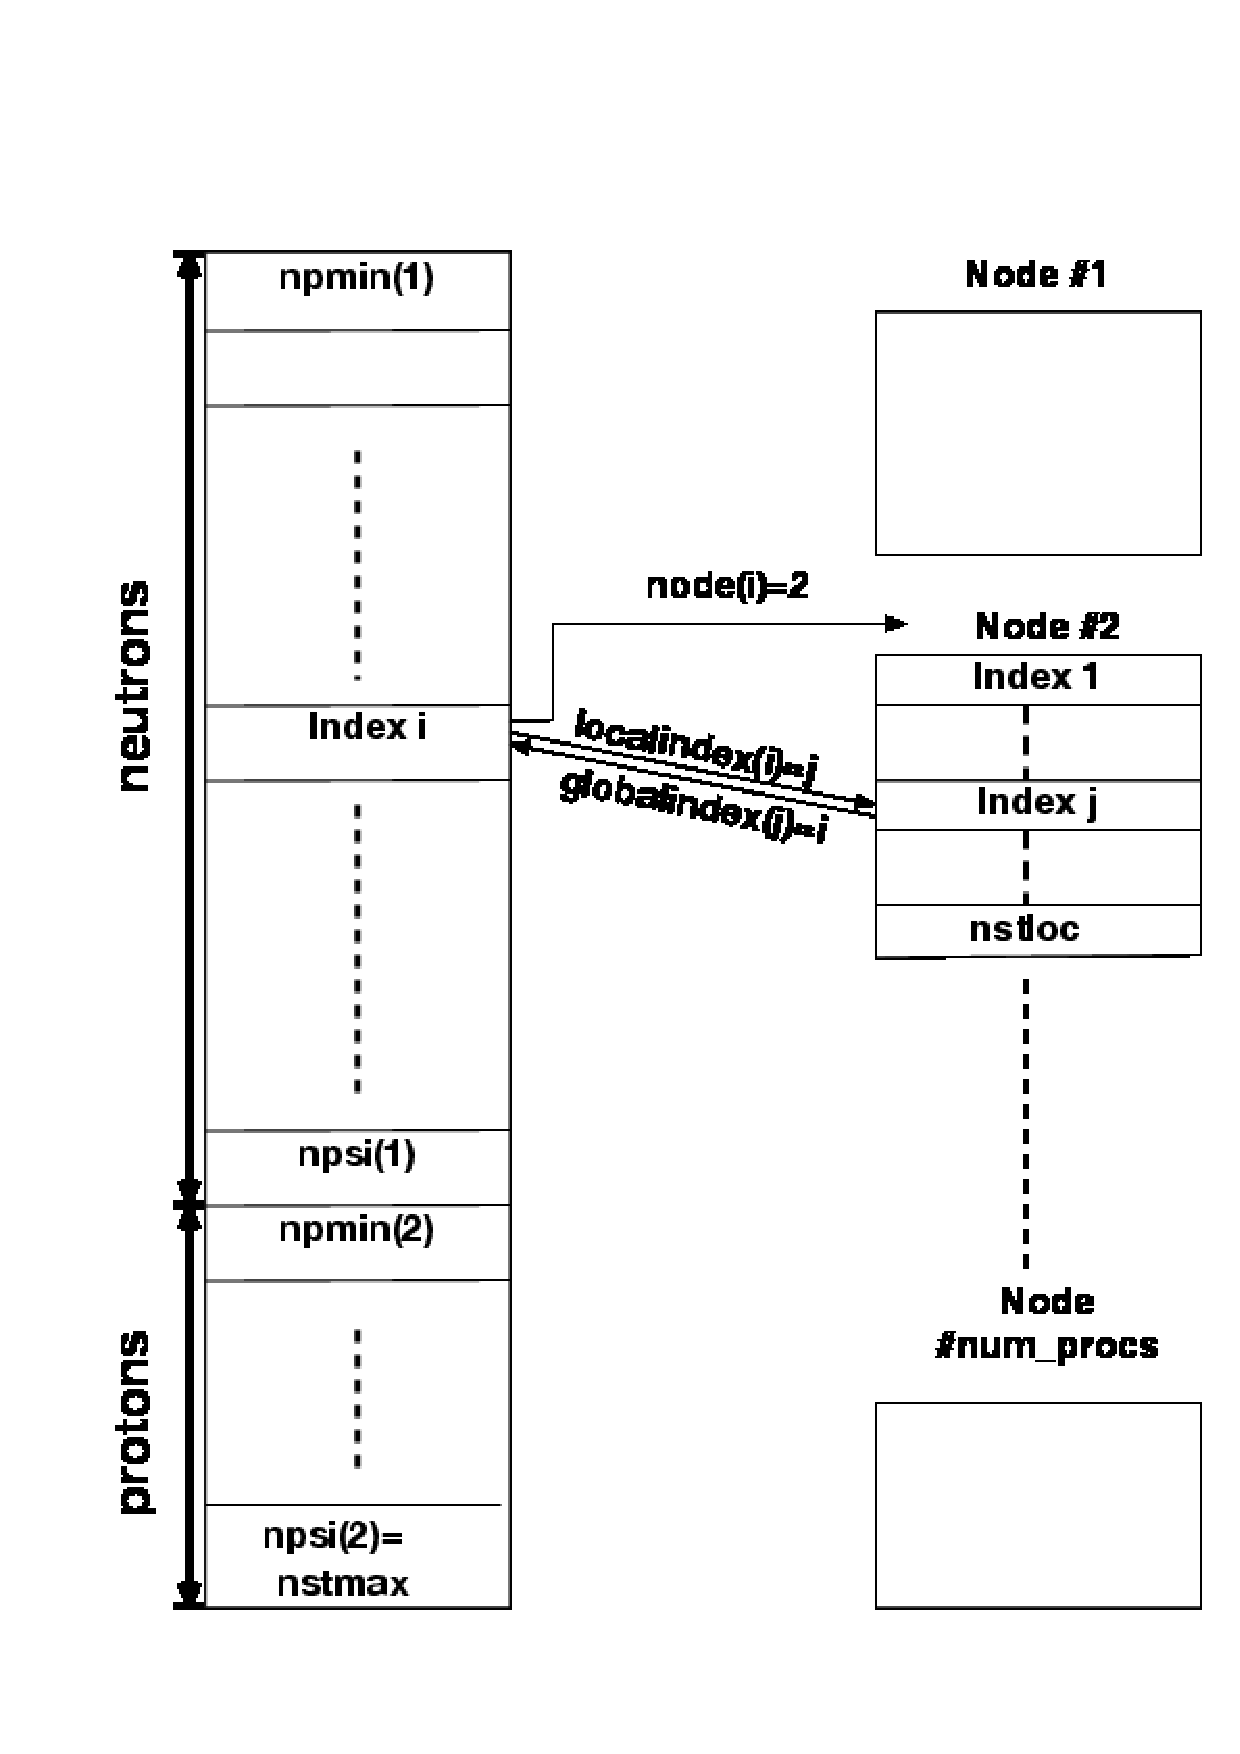
\includegraphics[width=0.7\linewidth]{Wavefun.pdf}}
\caption{\label{fig:wavefun}
Storage arrangement of the single-particle wave functions. On the left
the case for single-processor or {\tt OpenMP} is shown, which for the
case of distributed memory under {\tt MPI} is mapped to the individual
processors as shown on the right. Note that each node will have its
own values of {\tt nstloc} and {\tt globalindex}.
}
\end{figure}

If the code is run in parallel (MPI) on several nodes, only {\tt nstloc}
single-particle wave functions are stored on a given node, where {\tt
  nstloc} may vary. Pointers are then defined to indicate the
relationship between the local index and that in the global array of
wave functions. For details see the section on parallelization; the
general layout is given in Fig.~\ref{fig:wavefun}.

There are a number of arrays containing the physical properties of the wave
functions, such as the single-particle energy. The names start with
{\tt sp\_} and they are defined in module {\tt Levels}. They are not
split up in the parallel case, but on each node only the pertinent
index positions are used.

\subsubsection{Densities and currents}
The various densities necessary for constructing the mean field are
actually kept in separate arrays and can be output onto data files for
later analysis (see subroutine {\tt write\_densities}). The
dimensioning is {\tt (nx,ny,nz,2)} with the last index referring to
isospin for scalar densities, so that {\tt rho(:,:,:,1)} is the
neutron density and {\tt rho(:,:,:,2)} the proton density. For vector
densities there is an additional index with values~1 to~3 for the
Cartesian direction, thus {\tt sdens(nx,ny,nz,3,2)} containing the
spin density in each direction for neutrons and protons.

Since it is often not necessary to keep the neutron and proton
contributions separate, subroutine {\tt write\_densities} has the option of
adding them up before output.

\subsection{Initialization}
\label{sec:init}
A particular strength of the code is its flexible initialization.
There are essentially three types of initialization, which can be
selected through the input variable {\tt nof}:

\begin{enumerate}
\item\label{it:iniho} {\bf Harmonic oscillator:} {\tt nof=0}: this is
  applicable only to static calculations. The initial wave functions
  are generated from harmonic oscillator states with initial radii
  {\tt radinx}, {\tt radiny}, and {\tt radinz} in the three
  directions. It is advisable to choose the three radii different to
  avoid being kept in a symmetric configuration for non-spherical
  nuclei. Note that this is a very simple initialization and has some
  defects; for example, the initial deformation is controlled more by
  the occupation of the oscillator states than by the radius
  parameters. This should eventually be replaced by, e.~g., Nilsson
  wave functions.

  For this case the type of nucleus is determined by the input numbers
  {\tt nneut} and {\tt nprot} giving the number of neutrons and
  protons, while {\tt npsi} can be used to add some unoccupied states
  (this sometimes leads to faster convergence).

\item\label{it:frag} {\bf Fragment initialization:} {\tt nof>0}: wave
  functions for a number {\tt nof} of fragments are read in and
  positioned in the grid at certain positions. The wave functions are
  read from files produced by the static code with the file names
  given by the input {\tt filename}, they are positioned at
  center-of-mass positions {\tt fcent} and given an initial velocity
  controlled by {\tt fboost}. The code determines the number of wave
  functions needed from these data files and also checks the agreement of
  Skyrme force and grid used. This initialization is used, e.g., for
  nuclear reactions (see Section~\ref{sec:react}). For details see the
  input description in Section~\ref{sec:fragini}.

  The number of fragments read in is arbitrary, but there are two
  special cases:
  \begin{itemize}
  \item for {\tt nof=1} a single fragment is read in. This can be
    useful for initializing with static wave functions to study
    collective vibrations in a nucleus using the TDHF mode.
  \item for {\tt nof=2} a special initialization can be done where the
    initial velocities are not given directly but computed from a
    center-of-mass energy {\tt ecm} and an impact parameter {\tt b}.
  \end{itemize}
  
\item {\bf User initialization:} a user-supplied routine {\tt
    user\_init} can be employed to set up the wave functions in any
  desired way. The only condition is that the index ranges etc.\ are
  set up correctly and the wave function array {\tt psi} is filled
  with the proper values. It was found useful, e.~g., to use initial
  Gaussians distributed in various geometric patterns for
  $\alpha$-cluster studies.
\end{enumerate}

\subsection{Restarting a calculation}\label{sec:restart}
Sometimes it is necessary to continue a calculation that was not run
to the desired completion because of a machine failure or because the
number of iterations or time steps was set too low. In such cases the
last wave function file with name {\tt wffile}, which is generated at
regular intervals of {\tt mrest} iterations or time steps, can be used
to initialize a continuation. The program handles this in a simple fashion: if
the logical variable {\tt trestart} is input as {\tt TRUE}, it sets up
an initialization with one fragment (read from the initialization file)
placed at the origin and with zero
velocity. The only other modifications to the regular setup are then
to take the initial iteration number and time from that file instead
of starting at zero, as well as suppressing some unneeded
initialization steps.

Restarting works for both static and dynamic calculations. To continue
a calculation that was stopped because the desired number of
iterations or time steps was reached, a new limit for these should be
provided in the input.

This flexible restart makes it possible to use a different grid for
the continuation in the sense that the grid spacings must agree, but
the new grid can be larger than the old one.

\subsection{Accuracy considerations}\label{sec:accuracy}
The grid representation and solution methods introduced above depend
on several numerical parameters. Their proper choice is crucial
for the accuracy and speed of the calculations. In this Section, we
want to briefly address the dependence on numerical parameters. An
extensive discussion of grid representations and static iteration is
found in~\cite{Blu92a}.

\begin{figure}[h]
\centerline{\includegraphics[width=\linewidth]{static-grid.pdf}}
\caption{\label{fig:static-grid} Binding energy (left) and
  r.m.s. radius (right) of $^{16}$O computed for the force SkI3 drawn
  as functions of grid spacing $\Delta x=\Delta y=\Delta z$. A
  logarithmic scale us used for $\Delta x$. The number of grid points
  has been chosen to keep the box size constant at $N_x\Delta x=24$
  fm.}
\end{figure}
Figure \ref{fig:static-grid} shows the sensitivity with respect to the grid
spacings $\Delta x$, $\Delta y$, $\Delta z$. The trend is the same for
both observables, energy and radius: The results have very high
quality and change very little up to $\Delta x=$ 0.75 fm. They quickly
degrade above that spacing. But even at $\Delta x=$ 1 fm, we still
find an acceptable quality which suffices for most applications,
particularly for large scale explorations. If high accuracy matters, 
$\Delta x\approx$ 0.75 fm should be chosen;  not much is gained 
by going to even finer gridding. This holds for
ground states and moderate excitations. High excitations and fast
collisions may require a finer mesh. Note that the maximum
representable kinetic energy is
$E_\mathrm{kin,max}=(\hbar^2/2m)(\pi/\Delta x)^2$, which amounts to
about 200 MeV for $\Delta x=$ 1 fm. The actual energies of interest
should stay far below this limit. It is an instructive exercise to
study uniform center-of-mass motion at various velocities to explore the
limits of a given representation.

The number of grid points $N_x=N_y=N_z$ in the tests of Figure
\ref{fig:static-grid} were chosen such that the box size was the same
in all cases.  The actual choice of $N_x$ depends sensitively on the
system, its size and separation energy. As a rule of thumb, the
density decreases asymptotically as
$\rho\propto\exp{(-2\sqrt{2m\varepsilon_N}r/\hbar)}$ where
$\varepsilon_N$ is the single particle energy of the least bound
state. One should aim for at least $\rho<10^{-8}\,{\rm fm}^{-3}$ at
the boundaries.

\begin{figure}
\centerline{\includegraphics[width=0.5\linewidth]{dynamic-grids.pdf}}
\caption{\label{fig:dynamic-grids} Time evolution of the quadrupole
  momentum for two different grid spacings $\Delta x=\Delta y=\Delta
  z$ and constant box size of 24 fm. The test case is $^{16}$O excited by
  an instantaneous boost computed with the force SkI3.}
\end{figure}
Figure \ref{fig:dynamic-grids} explores the effect of grid spacing for
dynamics. Two different spacings are compared for a quadrupole
oscillation following an instantaneous quadrupole boost. Practically
no difference can be seen for the ``safe choice'' $\Delta x=$ 0.75 fm
and the robust choice $\Delta x=$ 1 fm. Dynamical applications,
oscillations and collisions, are in general less demanding and can
be performed very well with $\Delta x=$ 1 fm. This is pleasing as dynamical
calculations are usually much more costly than purely static ones.

There are two parameters regulating the static iteration according to
Eq.~(\ref{eq:dampstep}), the damping energy {\tt e0inv} and the step
size {\tt x0dmp}. {\tt e0inv} should correspond to the depth of
the binding potential. The overall step size {\tt x0dmp} can be of
order of one if {\tt e0inv} is well chosen. Nuclear binding is very
similar all over the chart of nuclei. This allows to develop one safe
choice for nearly all cases. We recommend {\tt e0inv}$\approx 100$ MeV
together with {\tt x0dmp}$\approx 1/2$, reducing the latter slightly
if convergence problems appear. Of course,
 a few percent in iteration speed might be gained by fine-tuning these
parameters for a given case, but this is not worth the effort unless
large scale surveys for a given class of nuclei and forces are
planned.

\begin{figure}[htb]
\centerline{\includegraphics*[width=0.95\linewidth]{dynamicSV-energ.pdf}}
\caption{\label{fig:dynamicSV-energ} Time evolution of the binding energy
  of $^{16}$O after an excitation by a soft cos$^2$ pulse of width 20
  fm/c computed for the force SV-bas~\cite{Klu09a} with a grid spacing
  $\Delta x=0.75$ fm and box size of 24 fm. Results are shown for
  different sizes of time step {\tt dt} and different order of Taylor
  expansion {\tt m} of the exponential evolution. The left panel shows
  the full evolution from ground state energy to the excited
  energy. The right panels concentrate on the times after the pulse is
  over in a narrower energy range relevant for this excitation.}
\end{figure}

The time stepping using the exponential propagator has the two parameters,
step size {\tt dt} and order {\tt mxp}$=m$ of the Taylor expansion
(\ref{eq:timepower}) of the exponential. Intuitively, one expects that
small {\tt dt} and large {\tt mxp} improve the quality of the
step. An efficient stepping scheme, however, looks for the largest {\tt
  dt} and smallest {\tt mxp} which still provide acceptable and
stable results. It is hard to give general rules as good working
values for the parameters depend on all details of the actual calculation:
gridding, nuclei involved, excitation energy, and kind of
excitation. 

Figure \ref{fig:dynamicSV-energ} demonstrates the dependence of a
typical dynamical evolution on these time-stepping parameters. We
consider a time interval up to 1260 fm/c which is a long time for
heavy-ion collisions and just sufficient for a spectral analysis of
oscillations~\cite{Rei07a}. The excitation is done by a soft sin$^2$
pulse of finite extension in time. The energy increases during the
initial excitation phase, as can be seen from the left panel in the
figure. After the external pulse is over, energy conservation holds,
which is nicely seen at plotting resolution in the left
panel. Normalization should be conserved at all times.  Both
conservation laws serve as tests for the time step. Norm is conserved
up to at least six digits for all cases and times shown in Figure
\ref{fig:dynamicSV-energ}. The energy is more critical. The right
panels show the energy in a small window around the final energy after
the excitation phase is over. The right lower panel shows a variation
of the Taylor order $m$ for fixed time step. The most prominent effect
is the sudden turn to catastrophic failure for $m=6$. In fact,
propagation by approximate exponential evolution explodes sooner or
later in all cases. The art is to extend the stable interval by
a proper choice of the stepping parameters. It is plausible that the
cases with $m>6$ maintain stability longer because the exponential is
better approximated. It is surprising that $m=4$ is also stable over
the whole time interval. There seem to be subtle cancellations of
error going on. Considering the stable signals, we see very little
differences between the cases. One may generally be happy with low
$m$. It is mainly stability demands which could call for larger
$m$. Note that this is not a generic result.  Stability for a given
test case should be checked once in a while and particularly before
launching larger surveys.

The right upper panel in Figure \ref{fig:dynamicSV-energ} shows
results for different {\tt dt} (as we have seen, the $m$ values are
not important as long as we achieve stable results). Here we see a
clear dependence on the step size. The energies remain constant in the
average. But there are energy fluctuations and these depend
sensitively on {\tt dt}. Smaller {\tt dt} yields smaller fluctuations.
As far as one can read off from the figure, the amplitude of the
fluctuations shrink $\propto${\tt dt}$^2$. It depends on the intended
analysis to which level of precision the time
evolution should be driven. A value of {\tt dt}$\approx$ 0.4 fm/c will be acceptable in most
cases because the average trend remains far smaller than the
fluctuations. Here also it must be emphasized that this is not a
generic number. Forces with lower effective mass (SV-bas has
$m^*/m=0.9$) are more demanding and usually require smaller {\tt
  dt}. On the other hand, running propagation without the spin-orbit term
allows even larger time steps because the spin-orbit potential is the
most critical piece in the mean-field Hamiltonian. The mix of
$\mathbf{p}$ and $\mathbf{r}$ imposes high demands on the numerical
representations. We again strongly recommend running a few
tests when switching forces or excitation schemes.

\section{Code structure}
The code is completely modularized to provide as large a degree of
encapsulation as possible in order to ease modification. Most modules
read their operating parameters from an associated {\tt NAMELIST} and
have their local initialization routines. In addition, a modern style
of programming is used that employs a minimum number of local
variables and streamlined array calculations that make the code lines
very close to the physical equations being solved.

Here we give a brief overview over the modules and their purpose. The
source files containing the modules have the same names, but all in
lower case, with an extension of {\tt .f90}. The
higher-level modules are:

\begin{description}
\item{Main program}: It calls initialization routines, sets up the
  initial wave functions using either harmonic oscillator states or
  reading wave functions of static Hartree-Fock solutions from given
  input files (module {\tt Fragments}). It then calls either {\tt
    statichf} from module {\tt Static} or {\tt dynamichf} from module
  {\tt Dynamic} to run the calculation.
\item{Static}: This contains the code for the static iterations {\tt
    statichf} and the subroutine {\tt sinfo} to generate output of the
  results.
\item{Dynamic}: runs the dynamic calculation in {\tt dynamichf} and
  generates output in {\tt tinfo}. Also controls the inclusion of an
  external excitation implemented in module {\tt External}.
\item{Densities}: calculates the densities and current densities by
  summing over the single-particle states.
\item{Meanfield}: contains the central physics calculation: the
  computation of the components of the mean field (subroutine {\tt
    skyrme}) and the application of the single-particle Hamiltonian to
  a wave function (subroutine {\tt hpsi}).
\item{Coulomb}: calculation of the Coulomb potential.
\item{Energies}: calculation of the total energies and its various
  contributions. 
\item{External}: calculation of the action of an external potential or
  initial collective boost of the wave functions.
\item{Pairs}: Implementation of the pairing correlations in the BCS
  approximation.
\item{Moment}: calculation of moments and deformation parameters for
  the bulk density.
\item{Twobody}: attempts to divide up the system into two separated
  nuclei and to calculate their properties and relative motion.
\end{description}

The lower-level supporting modules are:
\begin{description}
\item{Params}: general parameters used throughout the code. 
\item{Forces}: defines parameters of the Skyrme force and the pairing
  interaction and constructs them according to input.
\item{Grids}: defines everything associated with the numerical grid
  and sets it up.
\item{Levels}: definition of the single-particle wave functions and
  elementary operations on them such as derivatives.
\item{Fragments}: controls the reading of static wave functions from
  precomputed data and setting them up in the grid.
\item{Inout}: contains the subroutines for I/O of wave functions and
  densities. 
\item{Trivial}: defines some very basic operations on wave functions
  and densities.
\item{Fourier}: sets up the transform plans for the {\tt FFTW3}
  package to calculate Fourier transforms of wave functions and
  densities.
\item{Parallel}: This comes in two versions. The source file {\tt
    parallel.f90} contains the routines to handle {\tt MPI} message
  passing, while {\tt sequential.f90} sets up essentially dummy
  replacements for sequential or {\tt OpenMP} mode.
\item{User}: contains a sample user initialization code which can be
  used as a template for more complicated setups.
\end{description}

\section{Parallelization}
For both OpenMP~\cite{Cha08aB} and MPI~\cite{none12} the code can be
run in parallel mode. Parallelization for the static mode works in
OpenMP but not in MPI: the reason is in the orthogonalization step
which is not easily amenable for distributed-memory parallel
computation. This should be worked on in the future.

MPI and OpenMP can be used jointly if there are computing nodes with
multiple processors.

In both cases parallelization is done over the wave functions. The
code applies the time-development operator or the gradient iteration, which use the fixed set
of mean-field components, to each wave function, and this can naturally be
parallelized. Computing the mean fields and densities by summing up
over single-particle wave functions is also easily parallelizable. 

The library {\tt FFTW3}~\cite{Fri05a} itself can also run on multiple
processors in parallel. This can be used in addition to OpenMP or MPI,
but was found to be helpful only in the sequential version of the
code.

\subsection{OpenMP}
The application of the subroutine {\tt tstep} for propagating one wave
function for one time step, and of {\tt add\_densities} for adding one
wave function's contribution to the mean fields is done in
parallel loops. The only complicating factor is that the densities,
being accumulated in several subsets, must be kept separate using the
{\tt REDUCTION(+)} clause of OpenMP. The summation cannot be done
internally in {\tt add\_densities}, because for the half time step the
wave functions are immediately discarded after adding their
contribution to the densities to avoid having to store the full set at
half time. Thus only the combined {\tt tstep}-{\tt add\_densities}
loop should be parallelized.

The OpenMP program version can be compiled using the appropriate
compiler option. A separate {\tt Makefile.openmp} is provided which
just contains the {\tt -fopenmp} option for the GNU compiler.  The
number of parallel threads is not set by the code: the user should set
the environment variable {\tt OMP\_NUM\_THREADS} to the desired number.

The user should also check compatibility of the locally installed {�tt
  LAPACK/BLAS} libraries with {\tt OpenMP}.

\subsection{MPI}
In principle MPI uses the same technique as OpenMP, parallelizing over
wave functions. In this case, however, each node contains only a
fraction of the wave functions. This has several consequences:
\begin{enumerate}
\item The time-stepping of the wave functions can be done
  independently on each node, but requires that the densities are
  broadcast to all nodes after each half or full time step by summing
  up partial densities from the nodes in subroutine {\tt
    collect\_densities}.
\item The other calculation that uses wave functions directly is that
  of the single-particle properties. These are calculated on each node
  for the wave functions present on that node and then collected using
  subroutine {\tt collect\_sp\_properties}.
\item Only one node must be allowed to produce output. This is
  regulated by choosing node \#0 and setting the flag {\tt wflag} to
  {\tt .TRUE.}\ on that node.
\item The saving of the wave functions is done in the following way:
  Node zero writes a header file containing the job information on
  file {\tt wffile}, then each node writes a separate file {\tt
    wwfile.001}, {\tt wwfile.002}, and so on up to the number of
  nodes. This avoids having to collect the wave functions on one node.
\item Using these parallel output files as fragment initialization or
  restart files is handled so flexibly that they can be read into a
  different nodal configuration or even a sequential run.
\end{enumerate}

The MPI version needs the appropriate compiler and linker calls for
the system used. The sequential or OpenMP versions are obtained simply
by linking with {\tt sequential.f90} instead of {\tt parallel.f90},
which replaces the MPI calls with a set of dummy routines and sets up
the descriptor arrays for the wave function allocation in a trivial
way.

The {\tt Makefile.mpi} shows the procedure; in practice systems differ
considerably and the user should look up the compilation commands for
his particular system.

\newpage
\section{Program unit descriptions}
\subsection{Program {\tt Main3D}} \Indexmb{Main3D}
This is the main program that organizes the reading of the input and
funnels the calculation into the correct subroutines.

It consists of a number of simple steps. They are:

\begin{itemize}
\item{\bf Step 1:} initialize {\tt MPI} in case of an {\tt MPI} parallel job.
Start reading from standard input  beginning with 
  namelist \Indexn{files} for any changes in the file names.

\item{\bf Step 2:} read the definition of the force to be used and set
  it up (for its parameters see Section~\ref{sec:efunc}).

\item{\bf Step 3:} read namelist \Indexn{main}, which contains the
  overall controlling parameters. The choice of \Indexv{imode} is used to
  set up \Indexv{tstatic} and \Indexv{tdynamic} as logical variables. In
  addition, if this is a restart, the number of fragments is set to
  one. The properties of this one fragment are then filled in in
  subroutine \Indexp{getin\_fragments}.

\item{\bf Step 4:} read the grid definition (see Section
  \ref{sec:griddef}).  With the dimensions known, all grid-based
  arrays (but not the wave functions) can be allocated and the
  initialization of the {\tt FFTW} system can be done.

\item{\bf Step 5:} the appropriate namelist is read for the static or
  dynamic case, defining some parameters in those modules.

\item{\bf Step 6:} determine wave function numbers. The way this is
  done depends on the choice of \Indexv{nof}. For positive {\tt nof}, the
  fragment files are consulted to find out the properties of each and
  add up the numbers. For {\tt nof=0} the numbers are taken from
  namelist \Indexn{static}, which was read before. If {\tt nof<0}, they
  are also given in namelist {\tt static}, but the wave functions will
  be replaced by user-calculated ones.

\item{\bf Step 7:} now that the numbers are known, the wave function
  distribution over nodes is computed or set to trivial for a
  sequential calculation, and the the arrays related with wave
  functions are allocated.

\item{\bf Step 8:} the initial values of the wave functions are
  calculated. For \Indexv{nof}{\tt>0} the wave functions are read from the
  fragment files and inserted into the proper positions (see Sections
  \ref{sec:react} and \ref{sec:fragini}). For {\tt nof=0} the routine
  \Indexp{harmosc} in module {\tt Static} is called to calculate
  harmonic-oscillator wave function, and for {\tt nof<0} the routine
  \Indexp{init\_user} does an arbitrary user initialization.

\item{\bf Step 9:} the mean-field arrays are zeroed and the Coulomb
  solver is initialized.

\item{\bf Step 10:} the calculation branches into either static or
  dynamic mode.

  In the static calculation, \Indexp{init\_static} just prints some
  information and sets up damping (see Section~\ref{sec:statiter}) and
  \Indexp{statichf} does the real calculation.

  In the dynamic case, the subroutine \Indexp{dynamichf} does all the
  work.

\item{\bf Step 11:} finally the {\tt MPI} system is terminated.

\end{itemize}


\subsection{Module {\tt Coulomb}}\Indexmb{Coulomb}
\label{sec:modcoul}
\subsubsection{Purpose}
This module offers the subroutine {\tt poisson}, which calculates the
Coulomb potential from the proton density. The two boundary conditions
allowed are distinguished by the value of the variable \Indexv{periodic}.
If it is true, the mesh is assumed to be periodic in all three
directions and the Poisson equation is solved using the $1/k^2$
Green's function in momentum space and assuming a homogeneous negative
background annulling the total charge (jellium approximation).
Otherwise the boundary condition is for an isolated charge
distribution. In this case the potential is calculated by the method
of doubling the grid in all directions with zero density, folding with
the $1/r$-potential in momentum space and then restricting to the
physical region~\cite{Eas79}.


\subsubsection{Details on the Coulomb solver for an isolated system}
\newcommand{\bnu}{\mbox{\boldmath$\nu$}}
\newcommand{\bmu}{\mbox{\boldmath$\mu$}}

The Coulomb solver follows the ideas of \cite{Eas79}. We summarize
here the way it is realized in the code without detailed proofs.

Two grids are used. We will call them here $\mathcal{G}_1$ and
$\mathcal{G}_2$. The grid $\mathcal{G}_1$ is our standard working grid
as given in eq. (\ref{eq:FT}). We repeat here the essentials
\begin{subequations}
\begin{align*}
\mathcal{G}_1:\;&
  \nu_x=1,...,{\tt nx}\;,\;
  \nu_y=1,...,{\tt ny}\;,\;
  \nu_z=1,...,{\tt nz}\;;\;
\nonumber\\&
  \mbox{coordinate spacing: } {\tt dx}, {\tt dy}, {\tt dz};
\nonumber\\&
  \mbox{momentum spacing: } 
  {\tt dk}_x
  =
  \frac{2\pi}{{\tt nx}\!\cdot\!{\tt dx}},
  {\tt dk}_y
  =
  \frac{2\pi}{{\tt ny}\!\cdot\!{\tt dy}},
  {\tt dk}_z
  =
  \frac{2\pi}{{\tt nz}\!\cdot\!{\tt dz}};
\end{align*}
\end{subequations}
The second grid amounts to a doubled box in each direction, thus
\begin{subequations}
\begin{align*}
\mathcal{G}_2:\;&
  \nu_x=1,...,2{\tt nx}\;,\;
  \nu_y=1,...,2{\tt ny}\;,\;
  \nu_z=1,...,2{\tt nz}\;;\;
\nonumber\\&
  x_{\nu_x}=(\nu_x\!-\!{\tt nx}){\tt dx}\,,\,
  y_{\nu_y}=(\nu_y\!-\!{\tt ny}){\tt dy}\,,\,
  z_{\nu_z}=(\nu_z\!-\!{\tt nz}){\tt dz}\,;
\nonumber\\&
  \mbox{momentum spacing: } 
  {\tt dk}_x
  =
  \frac{2\pi}{{2\tt nx}\!\cdot\!{\tt dx}},
  {\tt dk}_y
  =
  \frac{2\pi}{{2\tt ny}\!\cdot\!{\tt dy}},
  {\tt dk}_z
  =
  \frac{2\pi}{{2\tt nz}\!\cdot\!{\tt dz}};
\end{align*}
\end{subequations}
The momenta $k_{n_i}$ in $\mathcal{G}_2$ are arranged around $k=0$
similar as in $\mathcal{G}_1$, but with half spacing ${\tt dk}_i$.
For simplicity, we will use compact notation
$\mathbf{r}_{\bnu}=\left(x_{\nu_x},y_{\nu_y},z_{\nu_z}\right)$
and similarly for $\mathbf{k}_\mathbf{n}$.

First, the Coulomb solver has to be initialized by defining the
appropriate Greens function which is done on $\mathcal{G}_2$.
The two necessary steps are:
\begin{enumerate}
  \item
  Prepare the Greens function in $r$ space as
  \begin{equation*}
     G(\mathbf{r}_{\bnu})=\frac{e^2}{|\mathbf{r}_{\bnu}|} 
     \quad.
  \end{equation*}
Special consideration has to be given to the singularity of the $1/r$
potential. In the discretized version, the value at $\vec r=0$ should
be replaced by the average of $1/r$ over a cuboid of size $\Delta
x\times\Delta y\times\Delta z$. For equal spacing in all three
directions this would lead to a value of $2.38/\Delta x$. Practical
experimentation, however, showed that the underlying assumption of a
point charge can be improved by some smeared-out density for nuclear
applications; a value of $2.84/\Delta x$ was found to be optimal.  
We use the expression 
  \begin{equation}\label{eq:coulsing}
    G(0)
    =
    \frac{2.84\sqrt{3}}{\sqrt{{\tt dx}^2+{\tt dy}^2+{\tt dz}^2}}
    \quad.
  \end{equation}

  \item
   Prepare the Greens function in $k$-space by
   3D fast Fourier transformation (FFT) on the double grid $\mathcal{G}_2$.
   $\tilde{G}(\mathbf{k}_{\bmu})={\tt FFT}\{G(\mathbf{r}_{\bnu})\}$.
   The array $\tilde{G}(\mathbf{k}_{\bmu})$ is stored 
   for further continued use.
\end{enumerate}
Once properly prepared, the practical steps for computing
the Coulomb field ${U}_\mathrm{Coul}(\mathbf{r}_{\bnu})$ for a 
density $\rho(\mathbf{r}_{\bnu})$ given on $\mathcal{G}_1$ are
\begin{enumerate}
 \item
  Extend $\rho_{\bnu}$ from  $\mathcal{G}_1$ to  $\mathcal{G}_2$ 
  by zero padding:
  \begin{equation*}
   \rho_2(\mathbf{r}_{\bnu})
   =
   \left\{\begin{array}{lcl}
    \rho(\mathbf{r}_{\bnu}) 
    &\mbox{ if }& 1\leq \nu_i \leq {\tt n}i \mbox{ for } i\in\{x,y,z\}
   \\
    0 &\mbox{ else }
   \end{array}\right.
  \end{equation*}
 \item
  Fourier transform the density in  $\mathcal{G}_2$:
  \begin{equation*}
   \rho_2(\mathbf{r}_{\bnu})\quad\longrightarrow\quad
   \tilde{\rho}_2(\mathbf{k}_{\bmu})={\tt FFT}\{\rho_2(\mathbf{r}_{\bnu})\}
  \end{equation*}
 \item
  Compute solution in $k$-space by multiplication with the
  formerly prepared Greens function
  \begin{equation*}
    \tilde{U}_2(\mathbf{k}_{\bmu})
    =
    \tilde{G}_2(\mathbf{k}_{\bmu})\tilde{\rho}_2(\mathbf{k}_{\bmu})
  \end{equation*}
  \item
  Compute solution in $r$-space by Fourier back transformation
  in $\mathcal{G}_2$:
  \begin{equation*}
    U_2(\mathbf{r}_{\bnu})={\tt FFT}^{-1}\{\tilde{U}_2(\mathbf{k}_{\bmu})\}
  \end{equation*}

 \item
  Map to standard grid  $\mathcal{G}_1$:
  \begin{equation*}
   {U}_\mathrm{Coul}(\mathbf{r}_{\bnu})
   =
   U_2(\mathbf{r}_{\bnu})
   \quad\mbox{for}\quad
   \bnu\in\mathcal{G}_1
  \end{equation*}
\end{enumerate}

\subsubsection{Module variables}
\begin{description}
\item{{\tt nx2, ny2, nz2:}} (INTEGER,PRIVATE) dimensions of the grid
  on which the Fourier transform is calculated. For the periodic case
  they are identical to the regular dimensions, for the isolated case
  they are doubled.
\item{{\tt coulplan1, coulplan2:}} (INTEGER,PRIVATE) plans for {\tt
    FFTW} complex forward and reverse transforms with array dimensions
  depending on the boundary condition.
\item{\Indexvb{wcoul}:} the Coulomb potential as a three-dimensional
  array. Units: MeV.
\item{{\tt q:}} (COMPLEX,PRIVATE) array for the
  complex Green's function (isolated) or array of $1/r$ values. Its
  dimension also depends on the boundary condition.
\end{description}

\subsubsection{Subroutine {\tt poisson}}\Indexpb{poisson} 
This subroutine solves the Poisson equation by the Fourier method. For
the periodic case, this means to just Fourier transform, multiply by
$1/k^2$, and the transform back. Note that the coefficient for
momentum zero must be zero also: this means that the total charge in
the box vanishes, corresponding to the jellium approximation.

In the non-periodic case we use use the trick of doubling the box size
in every direction and then folding with $1/r$ my multiplying the
Fourier transforms. The result in the physical box is then the correct
solution for the boundary condition of zero potential at infinity.
The key to success is not to use simply $1/k^2$ for the Fourier
transform of $1/r$, but to compute it on the actual grid the same way
as the densities and potentials are transformed~\cite{Eas79}.

\subsubsection{Subroutine {\tt coulinit}}\Indexpb{coulinit} 
This subroutine does the necessary initialization. It calculates the
dimension for the Fourier transform depending on the boundary
condition, allocates the necessary arrays and sets up the {\tt FFTW}
plans.

Then it composes the array {\tt q}. For the periodic case this
contains the values of the Green's function $1/k^2$, with zero at the
origin, while for the isolated case it first calculates the inverse
shortest distance $1/r$ from the origin with indices (1,1,1), replaces
the value at the origin according to Eq.~(\ref{eq:coulsing}) and then
Fourier-transforms this to use it for folding the density with the
coordinate-space Green's function.

\subsubsection{Subroutine {\tt initiq}}\Indexpb{initiq}
This subroutine calculates the contributions of each Cartesian index
to $r^2$ and $k^{-2}$. This depends on the boundary condition.  For
the periodic case, the values of the momenta are given by
$$ k_i=\frac{2\pi}{n\Delta x}\bigl(0,\;1,\;2,\;\ldots \frac{n}2-1,\;
-\frac{n}2,\;-\frac{n}2+1,\;\ldots -1\bigr).
$$
For an isolated distribution the shortest distances to the point with
index 1 are calculated (periodicity used):
$$ d_i=d\bigl(0,\;1,\;2,\;\ldots \frac{n}2-1,\;
-\frac{n}2,-\frac{n}2+1,\;\;\ldots 1\bigr).
$$
The input is the dimension along the coordinate direction given, the
output is the one-dimensional array {\tt iq} containing these values
{\bf squared}.


\newpage
\subsection{Module {\tt Densities}} \Indexmb{Densities}
This module has two purposes: it defines and allocates the densities
and currents making up the mean field according to Sect.~\ref{sec:dens},
and also contains the subroutine \Indexp{add\_density} which accumulates
the basic densities over the single-particle wave functions.
Subroutine \Indexp{skyrme} in module \Indexm{Meanfield} then uses these
densities to build up the components of the single-particle Hamiltonian.

\subsubsection{Module variables}
\begin{itemize}
\item{\bf Scalar densities:} These are dimensioned {\tt (nx,ny,nz,2)},
  where the last index is~1 for neutrons and~2 for protons.
  \begin{description}
  \item{\Indexvb{rho}:} the density, separately for each isospin (in
    fm$^{-3}$).  The definition is:
    $$ \rho_q(\vec r)=\sum_{k\in q}w_k^2\sum_s|\phi_k(\vec r,s)|^2,\qquad
    q=n,p $$
  \item{\Indexvb{tau}:} the kinetic energy density, also separately
    for each isospin. It is defined as the sum of the spin
    contributions and all particles of the given isospin
    $$ \tau_q(\vec r)=\sum_{k\in q}w_k^2\sum_s|\nabla\phi_k(\vec r,s)|^2,
    \qquad q=n,p$$ Note that it does not include the factor
    $\hbar^2/2m$. Units: fm$^{-5}$.
  \end{description}
\item{\bf Vector densities} These are dimensioned {\tt
    (nx,ny,nz,3,2)}, where the last index is~1 for neutrons and~2 for
  protons, and the next-to-last stands for the Cartesian direction.
  \begin{description}
  \item{\Indexvb{sdens}:} the spin density. It is defined as
    $$\vec\sigma_q(\vec r)=
    \sum_{\alpha\in q} w_\alpha^2 \sum_{ss'}\psi_\alpha^*(\vec
    r,s)\,\sigma_{ss'} \,\psi_\alpha(\vec r,s').$$ Note that it does
    not include the factor $\hbar/2$. Units: fm$^{-3}$.
  \item{\Indexvb{current}:} this is the total probability current
    density, defined in the familiar way as
    $$ \vec\jmath_q(\vec r)
    = \frac{1}{2\I}\sum_{\alpha\in q}w_\alpha^2
    \sum_s\left(\psi_\alpha^*(\vec r,s)\nabla\psi_\alpha(\vec
      r,s)-\psi_\alpha(\vec r,s) \nabla\psi_\alpha^*(\vec r,s)\right).
    $$
    Note that the factor $\frac{\hbar}{m}$ is not included. Its units
    are therefore fm$^{-4}$.
  \item{\Indexvb{sodens}:} the spin-orbit density, defined as
    $$ \vec J_q(\vec r)=\frac{1}\I\sum_{\alpha\in q}w_\alpha^2
    \sum_{ss'}\left(\psi_\alpha^*(\vec r,s)\nabla\times\sigma_{ss'}
      \psi_\alpha(\vec r,s')\right).
    $$
    Its units are also fm$^{-4}$.
  \end{description}
\end{itemize}

\subsubsection{Subroutine {\tt alloc\_densities}}
\Indexpb{alloc\_densities}
This is simply a short routine to allocate all the arrays defined in
this module.

\subsubsection{Subroutine {\tt add\_density}}
\Indexpb{add\_density}
This subroutine is given a single-particle wave function {\tt psin}
with its isospin index {\tt iq} and occupation $w_\alpha^2=${\tt weight} and adds
its contribution to the density arrays.

The reason for not including the loop over states in the subroutine is
that in the dynamic code, the contribution of a new single-particle
wave function (calculated by \Indexp{tstep}) to the densities is added
without saving that wave function, eliminating the requirement for a
second huge wave-function array.

It may seem strange that {\tt add\_density} has the densities
themselves as parameters, which are readily available in the module.
The reason for this is {\tt OPENMP} parallelization. The loop over
wave functions is done in parallel under {\tt OPENMP}. Since any of
the parallel tasks must add up the contributions of its assigned wave
functions, each task must have a copy of the densities to work on;
otherwise they would try to update the same density at the same time.
The separate copies are then combined using the {\tt OPENMP} {\tt
  REDUCE(+)} directive.

The local copies of the densities passed as arrays are denoted with
the prefixed letter ``l'' for {\em local}; they are {\tt lrho}, {\tt
  ltau}, {\tt lcurrent}, {\tt lsdens}, and {\tt lsodens}.

If the weight is zero, there is nothing to do and the subroutine
returns immediately. Otherwise, the contributions not involving
derivatives are first computed and added to the affected densities,
i.~e., number and spin density.

After this the derivative terms are evaluated by computing each
Cartesian direction separately. In all three cases the derivative is
evaluated first and put into {\tt ps1}, after which the contributions
are added straightforwardly. They involve the wave function itself,
the derivative, and for the spin-orbit density also a Pauli matrix, so
that different spin projections have to be combined properly.

The complex products always in the end evaluate to something real and
the expressions are simplified to take this into account. For example,
the following transformation is done: 
\begin{eqnarray*}
  \frac{1}{2\I}(\psi^*\nabla\psi-\psi\nabla\psi^*)&=&
  \frac{1}{2\I}\left(\psi^*\nabla\psi-(\psi^*\nabla\psi)^*\right)\\
  &=&\frac{1}{2\I}\left(2\I\Im(\psi^*\nabla\psi)\right)\\
  &\rightarrow&{\tt AIMAG(CONJG(psin)*psi1)}
\end{eqnarray*}
and similarly for the other expressions.

The efficiency of this relies on the FORTRAN compiler recognizing that
only the imaginary part of the complex product is needed and not
computing the real part at all. This seems to be the case with all
present compilers.

\newpage
\subsection{Module {\tt Dynamic}}\Indexmb{Dynamic}
This module contains the routines needed for time propagation of the
system (see Section~\ref{sec:timevol}). All the logic needed for this
case is concentrated here; all other modules except for \Indexm{External}
are equally used in the static calculation.

\subsubsection{Module variables}

\begin{itemize}
\item \Indexvb{nt}: the number of the final time step to be
  calculated. In case of a restart this is smaller than the total
  number of time steps.
\item \Indexvb{dt}: the physical time increment in units of fm/c.
\item \Indexvb{mxpact}: the number of terms to be taken in the
  expansion of the potential according to Eq.~(\ref{eq:timepower}).
\item \Indexvb{rsep}: the final separation distance. The calculation
  is stopped if there has been a reseparation into two fragments and
  their distance exceeds {\tt rsep}.
\item \Indexvb{texternal}: this logical variable indicates that an
  external field is present. See module {\tt External}.
\item \Indexvb{text\_timedep}: this logical variable indicates that the
  external field is time-dependent and does not describe an
  instantaneous boost.
\item \Indexvb{esf}: this is the energy shift for the call to {\tt
      hpsi}. Since it is not used in the dynamics part of the code, it
    is here set to the constant value of zero.
\end{itemize}

\subsubsection{Subroutine {\tt getin}\_dynamic}
\Indexpb{getin\_dynamic}
This is a relatively simple routine that reads the input for namelist
\Indexn{dynamic} and prints it on standard output. If \Indexv{texternal} is
true, it also calls \Indexp{getin\_external} to read the external field
parameters.

\subsubsection{Subroutine {\tt dynamichf}}\Indexpb{dynamichf}
This subroutine performs the main time-integration algorithm starting
at time step 0 and then iterating the desired number of steps. Its
building blocks are:
\begin{itemize}
\item {\bf Step 1: preparation phase}: this phase consists of several
  substeps. 
  \begin{enumerate}
  \item If this is not a restart, the time and iteration number are
    zeroed (for a restart only the physical time is taken from the
    {\tt wffile}). The wave functions are saved in the
    \Indexv{wffile}, to save setup time in case the calculation has to
    be restarted from this initial point.
  \item The instantaneous external boost (\ref{eq:extboost}) is applied using 
    \Indexp{extboost}. If this subroutine has applied a boost, it sets 
    \Indexv{text\_timedep} to {\tt .FALSE.} so no further calls to
    external-field routines are made (except for {\tt print\_extfield}).
  \item The protocol files {\tt *.res} are initialized with
  their header lines.  
 \item The densities and current are calculated in a loop over wave
    function by calling \Indexp{add\_densities}. 
    They are first set to zero and then accumulated in a
    loop over the set on the local node, followed by collecting them
    over all nodes.
  \item The mean field and (if {\tt texternal} is true) the
    external field are calculated for time zero using routines 
    \Indexp{skyrme} and \Indexp{extfld}.
  \item Then \Indexp{tinfo} is called to calculate and print the
    single-particle quantities and the total energies at time 0 or
    iteration~0.
  \item Finally preparations are made for the time-stepping loop: the
    starting index is set to iter+1: this is either after the end of a
    previous job in the case of a restart, or just one for a new
    calculation. The physical time is either~0 or the time taken from
    a restart file.
  \end{enumerate}

\item{\bf Step 2: predictor time step}: the loop over the iteration
  index {\tt iter} is started. Then the densities and mean-field
  components are estimated, i.~ e., in effect the Hamiltonian $\hat
  h(t+\tfrac1{2}\Delta t)$ required by the numerical method (see
  Eq.~(\ref{eq:midstep}) and Section~\ref{sec:timevol}). This is done
  by evolving the wave functions for a full {\tt dt} using the old
  Hamiltonian and averaging the densities between old and new ones to
  obtain the mid-time Hamiltonian for propagation. In detail the
  procedure is as follows:
  \begin{enumerate}
  \item The densities are not set to zero in order to allow  adding the
    contributions of the wave functions at the end of the time step.
  \item In the MPI version, the densities are divided by the number of
    nodes. In this way, adding up contributions from all nodes, the
    densities from the beginning of the time step will be included
    correctly.
  \item Subroutine \Indexp{tstep} is used to propagate the wave functions
    to the end of the time step. Note that truncation in the
    exponential happens at \Indexv{mxpact/2}, since the accuracy need not
    be as high as in the full step. For each wave function its
    contribution is added to the densities. The wave functions
    themselves do not need to be saved as they are not used for
    anything else.
  \item After the loop, contributions from all the nodes are added up
    for the MPI case using subroutine \Indexp{collect\_densities}.
  \item The densities are multiplied by one half to form the average
    of the values at $t$ and $t+\Delta t$.
  \item These average densities are then used to calculate the mean
    field at half time using subroutine \Indexp{skyrme}; also the
    external field is obtained for the half time using \Indexp{extfld}.
  \end{enumerate}

\item {\bf Step 3: full time step}: Now that the single-particle
  Hamiltonian has been estimated for the middle of the time step, the
  propagation can be carried out to the end of the time step. This is
  quite analogous to the half step with only three crucial
  differences:
  \begin{enumerate}
  \item The densities are reset to zero before the wave function loop,
    so the densities summed up are the purely the densities at the end
    of the time step,
  \item the series expansion in \Indexp{tstep} now uses the full 
    \Indexv{mxpact} terms, and
  \item the new wave functions are copied back into \Indexv{psi} to be
    available for the next time step.
  \end{enumerate}

\item {\bf Step 4: Center-of-mass correction}
If a center-of-mass correction is desired by the user by setting
\Indexv{mrescm}{\tt /=0}, 
subroutine \Indexp{resetcm} is called every {\tt mrescm}'th time step to
reset the center-of-mass velocity to zero.  

\item {\bf Step 5: generating some output} {\bf At this point the time is
    advanced by {\tt dt} because the physical time is now the end of
    the time step, and this must be printed out correctly by the
    following output routines.} \Indexp{tinfo} is called to calculate
  single-particle properties, total energies, and so on.

\item{\bf Step 6: finishing up the time step}: {\tt tinfo} is called
  to output the calculated data, then \Indexp{skyrme} and \Indexp{extfld}
  calculate the mean field and the external field, respectively, for the
  end of the time step, after which the wave functions are written
  onto \Indexv{wffile} depending on \Indexv{mrest}.
\end{itemize}
This ends the time loop and subroutine {\tt dynamichf} itself.

\subsubsection{Subroutine {\tt tstep}} \Indexpb{tstep}
In this subroutine one wave function given as the argument {\tt psout}
is stepped forward in time by the interval {\tt dt}. The method used
is the expansion of the exponential time-development operator
according to Eq.~(\ref{eq:timepower}), cut off at the power of {\tt
  mxp}, which in practice is usually around~6. Suppressing the argument of $\hat
h$ for brevity, we can write
\begin{equation}
  \label{eq:timepower2}
  \hat U(t,t+\Delta t)\,\phi\approx 
  \sum_{n=0}^m \phi^{(n)}
\end{equation}
with
\begin{equation}
  \phi^{(0)}=\phi,\qquad \phi^{(k+1)}=\frac{-\I\,\Delta t}{\hbar c
    k}\,\hat h\,\phi^{(k)},
  \quad k=0,\ldots,m-1.
\end{equation}

Thus the application of the polynomial to a single-particle wave
function can be evaluated simply in a loop applying $\hat h\phi_k$
repeatedly and accumulating the results in wave function {\tt psout}.

The argument {\tt iq} is only necessary because {\tt hpsi} needs
information about the isospin of the wave function.

\subsubsection{Subroutine {\tt tinfo}} \Indexpb{tinfo}
\label{sec:info}

This subroutine is used to output various pieces of information
relevant especially to the dynamic mode of the code. It is called at
the end of the full time step and consists of the following steps:
\begin{itemize}
\item {\bf Step 1: initialization}: the flag \Indexv{printnow} is
  calculated to keep track of whether this is the proper time step for
  a full printout (determined by \Indexv{mprint}).
\item {\bf Step 2: twobody analysis} the twobody analysis is
  performed, but only if the calculation started as a twobody
  scenario.

\item {\bf Step 3: moments}: the moments of the distribution are
  calculated using subroutine {\tt moments}. This includes total mass,
  momenta, and angular momenta. They are printed out if indicated by
  \Indexv{printnow}, both on the large output and in the specialized
  files \Indexv{dipolesfile}, \Indexv{momentafile}, and
  \Indexv{spinfile}. If there is an external field, the routine
  \Indexp{print\_extfield} is called to print the current expectation
  value of  the external field.

  {\bf Note that the moments need to be calculated every time step,
    because some of the logic may depend on them, especially the
    twobody-analysis, which needs the correct c.m., for example and is
    calculated at every time step and on every node.}
 
\item {\bf Step 4: single-particle quantities}: the single-particle
  energies are calculated straightforwardly as expectation values 
  of the Hamiltonian.
  The routine \Indexp{sp\_properties} is then called to obtain the other
  single-particle properties like angular momenta. They are
  communicated between the processors. The angular momenta are written
  to \Indexv{spinfile}.
\item{\bf Step 5: total energies}: The integrated energy \Indexv{ehfint}
  and its contributions are calculated in \Indexp{integ\_energy}. The
  subroutine {\tt sum\_energy} is called to calculate the three-body
  energy and the single-particle based total energy {\tt ehf}. The
  collective kinetic energy \Indexvb{ecoll} is computed directly
  here, because it is needed only in the dynamic calculations and only
  for output. It is defined as
  \begin{equation}
    \label{eq:ecoll}
    E_{\rm coll}=\frac{\hbar^2}{2m}\int \D^3r \frac{{\vec \jmath\,}^2}{\rho}
  \end{equation}
  The energies are protocolled in \Indexv{energiesfile} and on standard
  output.

\item {\bf Step 6: density output}: at intervals of \Indexv{mprint} or in
  the first time step the density printer plot is generated using 
  \Indexp{plot\_densities} and the binary densities are written onto {\tt *.tdd}
  files using \Indexp{write\_densities}.

\item {\bf Step 7: other output}: in the proper \Indexv{mprint} interval
  the two-body analysis results, the single-particle state
  information, and the moments are printed on standard output, using
  also the routines \Indexp{twobody\_print} and
  \Indexp{moment\_print}. 

  It is important to note that when {\tt
    tinfo} is called before the time step iteration starts, the
  two-body analysis cannot work because the fragment centers of mass
  from the previous time step  are either not known yet (restart) or
  identical to the present ones (initialization). The subroutine {\tt
    twobody\_case} is still called to find the fragment properties,
  but the derived kinetic energy etc.\ will be incorrect. Therefore
  the call to {\tt twobody\_print} is suppressed in this case. The
  logical variable {\tt initialcall} is used to recognize this case.


\item {\bf Step 8: check for final separation}: for the twobody case
  it is checked whether the separation found between the two fragments
  is larger than the input quantity \Indexv{rsep} with positive time
  derivative \Indexv{rdot} of the separation distance, in which case the
  program is terminated with an appropriate message.
\end{itemize}

\subsubsection{Subroutine {\tt resetcm}}\Indexpb{resetcm}
This subroutine resets the center-of-mass velocity to zero. The
velocity, or rather the corresponding wave vector, is calculated from
the current density using
\begin{equation*}
\rho(\vec r)  \vec k=\frac{1}{2\I}\sum_{\alpha\in q}w_\alpha^2
    \sum_s\left(\psi_\alpha^*(\vec r,s)\nabla\psi_\alpha(\vec
      r,s)-\psi_\alpha(\vec r,s) \nabla\psi_\alpha^*(\vec r,s)\right).
\end{equation*}
The wave functions are then multiplied by a common plane-wave phase
factor $\exp(-\I\vec k\cdot \vec r)$ to give a counter boost.

\newpage
\subsection{Module {\tt Energies}}\Indexmb{Energies}
This module computes the total energy and the various contributions to
it in two ways. The first method evaluates the density functional, 
Eq.~(\ref{eq:efundet}), by direct integration to compute the {\em integrated
  energy} {\tt ehfint}. The second method uses the sum of
single-particle energies plus the rearrangement energies, $E_{3,\rm
  corr}$ for the density dependent part and $E_{C,\rm corr}$ for
Coulomb exchange as explained in Section~\ref{sec:alterenerg}.

The two ways of calculating the energy are assigned to the subroutines
{\tt integ\_energy}, which also calculates the rearrangement energies,
and {\tt sum\_energy}. Note that since {\tt integ\_energy} is always
called briefly before {\tt sum\_energy}, the rearrangement energies
are correctly available.

In addition subroutine {\tt sum\_energies} also calculates the summed
spin, orbital, and total angular momenta.

\subsubsection{Module variables}
\label{sec:modvar}
All the variables in this module are given in MeV unless otherwise
noted.
\begin{itemize}
\item \Indexvb{ehft} denotes the total kinetic energy of 
Eq.~(\ref{eq:ehft}).
\item \Indexvb{ehf0} corresponds to the $b_0$ and $b_0'$-dependent
  terms of Eq.~(\ref{eq:ehf0}).
\item \Indexvb{ehf1}: the contribution depending on $b_1$ and $b_1'$
  of Eq.~(\ref{eq:ehf1}).
\item \Indexvb{ehf2} accounts for the $b_2$, $b_2'$-dependent
  contributions of Eq.~(\ref{eq:ehf2}).
\item \Indexvb{ehf3} is the $b_3$, $b_3'$-dependent part of
 Eq.~(\ref{eq:ehf3}) which models density dependence.
\item \Indexvb{ehfls} is the spin-orbit energy (\ref{eq:ehfls}).
\item \Indexvb{ehfc} is the Coulomb energy of Eq.~(\ref{eq:ehfc}).
\item \Indexvb{ecorc} is the rearrangement correction
  (\ref{eq:ecorc}) to Coulomb exchange in the Slater approximation.
\item {\tt e3corr} is the rearrangement energy (\ref{eq:e3corr}) to
  the density-dependent part of the Skyrme energy.
\item \Indexvb{orbital}: the three components of the total orbital
  angular momentum in units of $\hbar$.
\item \Indexvb{spin}: the three components of the total spin in
  units of $\hbar$.
\item \Indexvb{total\_angmom}: the three components of the total
  angular momentum in units of $\hbar$.
\end{itemize}

\subsubsection{Subroutine {\tt integ\_energy}}\Indexpb{integ\_energy}
The purpose of this subroutine is to calculate the integrated energy
of Eq.~(\ref{eq:efundet}). This is implemented pretty straightforwardly
using the integrals defined in Section~\ref{sec:efunc}. The only
programming technique worth noting is that intermediate variables such
as {\tt rhot} for the total density are used to avoid repeating the
lengthy index lists. Compilers will eliminate these by optimization.

In principle the integration loops in the subroutine could be
combined, but some space is saved by using the array {\tt worka} for
different purposes in different loops.

The calculation proceeds in the following steps:

\begin{itemize}
\item {\bf Step 1}: the Laplacian of the densities is calculated in
  {\tt worka}, then the integrals of
  Eqs.~(\ref{eq:ehf0},\ref{eq:ehf2}, and \ref{eq:ehf3}) are performed.
  After the loop the result for {\tt ehf3} is also used to calculate
  {\tt e3corr} of Eq.~(\ref{eq:e3corr}).
\item {\bf Step 2}: the integral of Eq.~(\ref{eq:ehf1}) is evaluated
  using {\tt worka} for the $\vec\jmath_q{}^2$ term.
\item {\bf Step 3}: the spin-orbit contribution of 
Eq.~(\ref{eq:ehfls}) is calculated using {\tt worka} as storage for
  $\nabla\cdot\vec J_q$.
\item {\bf Step 4}: the Coulomb energy is evaluated from 
 Eq.~(\ref{eq:ehfc}) with the Slater correction taken into account if the
  force's \Indexv{ex} is nonzero. At the same time the Coulomb correction
  for the summed energy is calculated according to
  Eq.~(\ref{eq:ecorc}) and stored in {\tt ecorc}. It will be used in
  the subroutine {\tt sum\_energy}.
\item {\bf Step 5}: the kinetic energy is integrated for 
Eq.~(\ref{eq:ehft}). Note that only at this point the correct prefactor
  $\hbar^2/2m$ is added; the use of {\tt tau} in other expressions
  assumes its absence.
\item {\bf Step 6}: Finally all terms are added to produce the total
  energy, Eq.~(\ref{eq:efundet}), from which the pairing energies are
  subtracted.
\end{itemize}

\subsubsection{Subroutine {\tt sum\_energy}}
\Indexpb{sum\_energy}
This subroutine mainly computes the Koopman sum of 
Eq.~(\ref{eq:koopman}), but also sums up a number of other single-particle
properties. For systematics, the latter should be done in a different
place, but at present is left here.

The summation of the total energy uses Eq.~(\ref{eq:spenerg}) to
compute
$$ \sum_k (\epsilon_k-\tfrac1{2}v_k)=\tfrac1{2}\sum_k(2t_k+v_k)=
\tfrac1{2}\sum_k(t_k+\epsilon_k). $$ The last sum is calculated,
the rearrangement corrections are added and the pairing energies
subtracted.

The subroutine then sums up the single-particle energy fluctuation
\Indexv{sp\_efluct1} and \Indexv{sp\_efluct2}, dividing them by the nucleon
number.  Finally the orbital and spin angular
momentum components are summed to form the total ones.

\newpage
\subsection{Module {\tt External}}\Indexmb{External}
This module allows the coupling of the nucleonic wave functions to an
external field. As described in Sect.~\ref{sec:external}, this can be
done either by adding a time-dependent external (i.~e., not
self-consistent) potential to the single-particle Hamiltonian, or by
giving an initial ``boost'' to each wave function.. Since this is very
easy to modify and will probably have to be adjusted for most
applications, the present version just contains a sample for a
quadrupole coupling. The logic for different time-dependence
assumptions and the isospin are however, fully functional and should
be useful in many cases.

\subsubsection{Module variables}
Most of these just describe the behavior of the external field. They
are all declared as private, so that the user modifying this code can
be sure that the internals are not used anywhere else. The variables
are:

\begin{itemize}
\item{\Indexvb{amplq0}:} a strength parameter for the perturbation.
  As explained in Sect-~\ref{sec:external}, its numerical magnitude is
  usually not important by itself, but varying it allows studying the effects
  of different strengths of the excitation.
\item{\Indexvb{textfield\_periodic}:} if this is set to {\tt true}, the
    external field is made periodic according to
    Eq.~(\ref{eq:extperiodic}), otherwise a damping factor is used as
    defined in Eq.~(\ref{eq:extdamp}).
\item{\Indexvb{radext},\Indexvb{widext}:} parameters $r_0$ and
  $\Delta r$ for the cutoff of the field according to
  Eq.~(\ref{eq:extdamp}). Dimension: fm.
\item{\Indexvb{isoext}:} isospin behavior of the external field: {\tt
    isoext=0} denotes the same action on protons and neutrons, {\tt
    isoext=1} that with opposing signs.
\item{\Indexvb{ipulse}:} type of pulse. {\tt ipulse=0} denotes the
  initial boost configuration, {\tt ipulse=1} a Gaussian pulse
  according to Eq.~(\ref{eq:extgauss}), and {\tt ipulse=2} a cosine
  squared behavior as defined in Eq.~(\ref{eq:extcos}).
\item{\Indexvb{omega}, \Indexvb{tau0}, and \Indexvb{taut}:} these
  correspond to the parameters $\omega$, $\tau_0$, and $\Delta\tau$ in
  Eqs.~(\ref{eq:extgauss}) and (\ref{eq:extcos}).
\item{\Indexvb{extfield}:} this is the time-independent field
  generated according to the parameters {\tt amplq0}, {\tt
    textfield\_periodic}, and depending on the latter, possibly {\tt radext}
  and {\tt widext}. It is used either to calculate the initial boost
  or is added to the mean field multiplied with the time-dependent
  factor.
\end{itemize}

\subsubsection{Subroutine {\tt getin\_external}}
\Indexpb{getin\_external}
This is quite straightforward. It reads in all the parameters of the
external field and immediately does some consistency checks. The
relative strength for the neutron and proton fields is set equal for
{\tt isoext=0} but reduced by the corresponding number of particles in
the {\tt isoext=1}. This avoids a shift of the center of mass in this
case.

Then the array {\tt extfield} is allocated and the time-independent
spatial potential calculated for both isospin cases and in either the
periodic or damped versions, depending on the value of {\tt
  textfield\_periodic}.This is just an illustrative sample field of
type $Q_{zz}$; in a real calculation there is no need to provide both
versions.

\subsubsection{Subroutine {\tt extfld}}\Indexpb{extfld}
This is again a very straightforward routine. It calculates the
time-dependent prefactor {\tt time\_factor} depending on the
parameters, and adds the time-independent field {\tt extfield}
multiplied by this factor to {\tt upot}. The physical time is here
given as an argument, because it needs to be evaluated at both full
and half time steps.

\subsubsection{Subroutine {\tt extboost}}\Indexpb{extboost}
This performs the initial boost according to Eq.~(\ref{eq:extboost})
on all single-particle wave functions. Note that it is always called
from {\tt dynamichf} and checks itself whether {\tt ipulse} is zero.
This enables {\tt ipulse} to also be made a private variable. Its
argument is used to communicate whether it has actually done anything:
if it has applied a boost, it sets its argument to {\tt .FALSE.}  so that in {\tt
  dynamichf} the variable {\tt text\_timedep} makes it possible to
distinguish this case..

\subsubsection{Subroutine {\tt print\_extfield}}
\Indexpb{print\_extfield}
This subroutine calculates the expectation of the coupling energy to
the external field,
$$\sum_q\int\,\D^3r\,\rho_q(\vec r)F_q(\vec r)$$
and prints one line containing the present time and this value onto
the file \Indexv{extfieldfile}.

\newpage
\subsection{Module {\tt Forces}}\Indexmb{Forces}
\label{sec:Forces}
Module {\tt Forces} describes the interactions used in the code. The
idea is to produce a library of Skyrme forces that can be called up
simply by name, but for exploratory purposes a force can also be input
using individual parameter values. A force is usually fitted together
with a prescription for the pairing and center-of-mass correction, so
that these properties are here defined as part of the force.

\subsubsection{Module variables and types}
\label{sec:types}
To deal with forces and pairing as a unit, derived types are used:
\begin{itemize}
\item{\tt Pairing}: This contains the following parameters for
  pairing:
  \begin{description}
  \item[{\tt v0prot}]: the strength of pairing for protons in MeV.
  \item[{\tt v0neut}]: the strength of pairing for neutrons in MeV.
  \item[{\tt rho0pr}]: the density parameter for the density-dependent
    delta pairing (see description for module \Indexm{Pairs}).
  \end{description}
\item{\tt Force}: the description of a Skyrme force. It contains the
  following values:
  \begin{description}
  \item[name]: the name of the force used to identify it.
  \item[{\tt ex}]: some forces are fitted excluding the Coulomb
    exchange term. For {\tt ex=1} it is included (this is the normal
    case), for {\tt ex=0} not.
  \item[\Indexvb{zpe}]: index for the treatment of the center-of-mass
    correction (see end of Section~\ref{sec:efunc}).
  \item[\Indexvb{h2m}] value of $\frac{\hbar^2}{2m}$, separately 
    for neutrons and protons.
  \item[\Indexvb{t0}, \Indexvb{t1}, \Indexvb{t2}, \Indexvb{t3},
    \Indexvb{t4}]: Skyrme parameters $t_0$, $t_1$, $t_2$, $t_3$, and
    $t_4$. Defined in the usual way.
  \item[\Indexvb{x0}, \Indexvb{x1}, \Indexvb{x2}, \Indexvb{x3}]
    Skyrme exchange parameters $x_0$, $x_1$, $x_2$, and $x_3$.
  \item[\Indexvb{b4p}] spin-orbit modification parameter $b_4'$ 
    introduced in the ``SkI'' series of forces (see Sect.~{xx}).
  \item[\Indexvb{power}]: exponent in the nonlinear (originally
    three-body) term.
  \item[\Indexvb{vdi}]: parameter set for the volume-delta
    pairing case.
  \item[\Indexvb{dddi}]: parameter set for the
    density-dependent delta pairing case.
  \end{description}
\end{itemize}
The variables defined in the module are
\begin{itemize}
\item \Indexvb{ipair}: selects one of several pairing modes.  For
  historical reasons the values are 0: no pairing, 5: VDI pairing, and
  6: DDDI pairing. In the input the symbolic names are used so these
  numerical values are hidden to the user. For details see the input
  description and module \Indexm{Pairs}.
\item \Indexvb{f}: this contains parameters for
  the Skyrme force actually used in the present calculation, packed
  into the derived-type {\tt Force}.
\item \Indexvb{p} : the pairing parameters used in the
  present calculation. This is separate from the force itself: the
  force definition usually contains suggestions for the associated
  pairing, but this often overridden, e.g, by turning off
  pairing.
\item \Indexvb{h2ma}: the average of the two {\tt h2m} values for
  protons and neutrons.
\item \Indexvb{nucleon\_mass}: the mass of the nucleon (average of
  neutron and Proton) in MeV calculated from {\tt h2ma} and \Indexv{hbc}.
\item The {\tt b} coefficients: these are the coefficients actually
  used for the mean-field and single-particle Hamiltonian calculations
  in \Indexp{skyrme} and \Indexp{integ\_energy}. Note that only {\tt
    b4p} is also included in the Skyrme-force definition; the others
  are derived from the {\tt t} coefficients.
\end{itemize}


The predefined Skyrme forces are contained in {\tt forces.data}, which
contains an array {\tt pforce} of {\tt TYPE(Force)} data. This is a
bit unreliable since the Fortran standard restricts the length of
statements; it should be replaced by reading from a data file in case
this limit causes problems. The present version is, however, still preferred as
a data file would have to be replicated in every application directory
(or an absolute path would have to be defined in the {\tt OPEN}
statement).

\subsubsection{Subroutine {\tt read\_force}}\Indexpb{read\_force}
The purpose of the subroutine is to read the force and pairing
definitions. The {\tt NAMELIST} \Indexn{force} contains all the
defining values for a Skyrme force (but now as individual variables,
not in a derived type) plus a selection of pairing type and strengths
(see input description). In addition there is a logical variable
\Indexvb{turnoff\_zpe} which allows turning off the center-of-mass
correction.

Some quantities are first set negative to see whether required input
is missing. Then a predefined Skyrme force with the given name is
sought; if it is found, it is simply copied into {\tt f}. If no force
of this name is found, a new one is composed from the numbers given in
the input.

If the input varable \Indexv{turnoff\_zpe} is true, the indicator {\tt
  f\%zpe} is set to~1, which implies not doing anything about the
center-of-mass correction. Actually, in the current version this
affects only one statement in the static module.

Now the ``b'' coefficients as given in Eq.~(\ref{eq:force-coeff}) are
calculated straightforwardly.  There is one additional coefficient
{\tt slate} used for the Slater approximation to the Coulomb exchange
term. This is not a free parameter, but precomputed for convenience in
{\tt forces.f90}.  The $b$ and $b'$ coefficients are used in
subroutine \Indexp{skyrme} (module \Indexm{Meanfield}) and \Indexp{energy}
(module \Indexm{Energies}).

The variable {\tt pairing} from the namelist then determines the
pairing. If it is set to {\tt 'NONE'}, no pairing is
included. Otherwise the strength parameters are taken from the input
or from the predefined force. If this process does not find a
reasonable pairing combination, stop with an error message.


Finally the routine calculates the values of \Indexv{nucleon\_mass} and
\Indexv{h2ma}. It then prints out a description of the force and pairing
parameters.

\newpage
\subsection{Module {\tt Fourier}}\Indexmb{Fourier}
This module initializes the {\tt FFTW3} package for doing Fourier
transforms~\cite{Fri05a}. It needs the file {\tt fftw3.f} from the
{\tt FFTW3} package to define the symbolic parameters for the
initialization calls.

Note that {\tt FFTW} is used only for the complex transforms of the
wave functions and the Coulomb solver; the Fourier derivatives of the
real fields are handled by explicit matrix multiplication (see module
\Indexm{Trivial}, routines \Indexp{rmulx}, \Indexp{rmuly}, and \Indexp{rmulz}).
The definition of the plans for the Coulomb solver is contained in
subroutine \Indexp{coulinit} in module \Indexm{Coulomb}.

\subsubsection{Module variables}
The module variables describe the various {\tt FFTW} plans used in the
code.
\begin{description}
\item{\Indexvb{pforward}, \Indexvb{pbackward}:} plans for full
  three-dimensional forward and backward transforms for both spin
  components.
\item{\Indexvb{xforward}, \Indexvb{xbackward}:} one-dimensional
  forward and backward transform in the $x$-direction, but for all
  values of $y$, $z$, and spin $s$.
\item{\Indexvb{yforward}, \Indexvb{ybackward}:} one-dimensional
  forward and backward transform in the $y$-direction, but for all
  values of $x$, $z$, and spin $s$.
\item{\Indexvb{zforward}, \Indexvb{zbackward}:} one-dimensional forward
  and backward transform in the $z$-direction, but for all values of
  $x$, $y$, and spin $s$.
\end{description}

\subsubsection{Subroutine {\tt initfft}}\Indexpb{initfft}
In this subroutine the {\tt FFTW} system is initialized and a 2-wave
function array {\tt p} is allocated temporarily for performing the
tests to make the plans efficient (we do not use dynamic allocation,
since having this array on the stack may produce different results
than on the heap --- a point which has not been tested, though).

This is followed by the calls to set up the plans. These have
different variations, since the way in which the index or indices over
which the transform is done are intertwined with the unaffected
indices is quite different for the different directions. Understanding
this Section requires a thorough familiarity with the FFTW
documentation and Fortran indexing.

{\bf An important point to consider when modifying the code:} the
setting-up of a plan must agree with its later use with respect to
whether the input and output arrays are the same (in-place transform)
or different. This is why {\tt p} sometimes has a last index of 2 in
these calls: in the code all transforms are in-place except for {\tt
  xforward}, {\tt yforward}, and {\tt zforward}. It was found that
very strange things happen if this rule is not obeyed.

\newpage
\subsection{Module {\tt Fragments}}\Indexmb{Fragments}
\label{sec:fragini}
This module is concerned with setting up the initial condition from
data files containing fragment wave functions, usually obtained in a
previous static calculation. A typical application is the
initialization of a heavy-ion reaction, see Section~\ref{sec:react}.
Beyond that, any number of fragments (limited by the parameter
variable \Indexv{mnof}) can be put into the grid at prescribed positions
with given initial velocities. A condition is, however, that the grid
they are defined in is smaller than the new grid. If they are put
close to the boundary, they may have density appearing on the other
side because of periodicity; this may be acceptable if the boundary
condition is periodic. A calculation may be restarted on a larger
grid, but this may be accompanied by some loss of accuracy, since the
wave function outside the original regions is set to a constant small value.

For the case of parallel {\tt MPI} calculations, there is logic to read wave functions
distributed over a series of files as described in connection with
subroutine \Indexp{write\_wavefunctions}. Since only the dynamic case
can run under {\tt MPI} at present, the only application of this is to
restart a dynamic calculation. The number of processors may be
different in the restart.

\subsubsection{Module variables}
\begin{description}
\item[\Indexvb{fix\_boost} (input)]: if this is set to true, the boost
  (initial kinetic energy) values are used unchanged from the input;
  otherwise they are calculated from the initial kinetic energy of
  relative motion {\tt ecm} and the impact parameter {\tt b}. This
  implies a two-body initial configuration. The initial motion is
  assumed to be in the $(x,z)$-plane in this case.  Note that for two
  initial fragments fix\_boost can also be set to true for special
  initial conditions.
\item[\Indexvb{filename} (input)]: for each fragment this indicates the
  name of the file with the associated wave functions. One file can be
  used several times in the case of identical fragments, abut the code
  does not treat that as a special case.
\item[\Indexvb{fcent} (input)] for fragment no. {\tt i} the initial
  three-dimensional position is determined by {\tt fcent(:,i)}.
\item[\Indexvb{fboost} (input)] gives the initial motion {\tt
    fboost(:,i)} of fragment {\tt i} in 3 dimensions. This is not a
  velocity, but the total kinetic energy of the fragment {\em in that
    Cartesian direction} in MeV. The sign indicates the direction,
  positive or negative along the corresponding axis. The sum of
  absolute values thus is the total kinetic energy of the fragment. These
  values are used only if {\tt fix\_boost} is true.
\end{description}
The following variables are used only if fix\_boost is false, i.~e.,
for two-body initialization from relative motion.
\begin{description}
\item[\Indexvb{ecm}, \Indexvb{b} (input)] The kinetic energy of
  relative motion in MeV and the impact parameter in fm.
\item[{\tt vx}, {\tt vz}] The components of the relative velocity in
  the $(x,z)$-plane
\item[{\tt xli}] The angular momentum of relative motion in units of
  $\hbar$.
\end{description}
The following quantities have names of other variables prefixed by an
``f'' and {\em are indexed by fragment number}; for the most part they duplicate
variables describing the whole system on a fragment-by-fragment basis.
\begin{description}
\item[{\tt fcmtot}, {\tt fmass}, {\tt fcharge}] Centers of mass, masses,
  and charges of the fragments.
\item[{\tt fnneut}, {\tt fnprot}, {\tt fnstmax}, {\tt fnpmin}, {\tt
    fnpsi}] These have the same meaning as the variable without ``f'',
  but apply to the set of wave functions for one specific fragment.
\item[{\tt fnumber}] gives the number of wave functions in the
  fragment for each isospin. For initialization of a dynamic
  calculation only wave functions with a nonzero occupation are taken
  into account.
\item[{\tt fnewnpmin}, {\tt fnewnpsi}] are the starting and ending
  indices for each fragment's wave functions in the total set of
  wave functions combining all the fragments.
\item[{\tt fnx}, {\tt fny}, {\tt fnz}] indicate the grid size on which
  the fragment wave functions are defined.
\item[{\tt fnode} and {\tt flocalindex}] are used for MPI. When the
  wave functions were written by the parallel code, each node produced
  a file named ``{\em nnn}{\tt .wffile}'', which contains the wave
  functions present on that node. For the wave function with index {\tt
    nst}, {\tt fnode(nst)} indicates the number of the file and {\tt
    flocalindex(nst)} the position in the file. These are analogous to
  the variables \Indexv{node} and \Indexv{localindex} for the complete
  calculation and are explained more thoroughly in the description of
  module \Indexm{Parallel}, see section~\ref{sec:parallel}.
\end{description}
  
\subsubsection{Subroutine {\tt getin\_fragments}}
\Indexpb{getin\_fragments}
This subroutine reads the input variables, makes some consistency
checks, and then prepares for the initialization.

A restart is set up by placing one fragment taken from {\tt wffile} at
the origin with zero velocity (see Sect.~\ref{sec:restart}).

The main loop is over fragments. The fragment files are opened a first
time to obtain information about the fragments, which is stored in
fragment-specific arrays. The checks include agreement of the forces
and grid spacings as well as that the fragment grid is not larger than
the new grid.

The code at this point makes a distinction between static and dynamic
modes: for a static calculation it is assumed that the data may be
needed for a restart. In this case all wave functions are read in even
if not occupied even fractionally. For the dynamic case only those
with non-zero occupation are input as determined from \Indexv{fwocc}.
This yields a reduced value for \Indexv{fnumber}.

{\bf Note that at present it is assumed that the static wave functions
  are ordered in ascending energy, so that the occupied ones will
  start at index one and all empty states will be at the uppermost
  index positions.}

Following this, the index positions in the new wave function array are
calculated in \Indexv{fnewnpmin} and \Indexv{fnewnpsi} by adding the
numbers of wave functions of each fragment-specific successively. Note
that at this stage the proton indices are still counted from one.

After this input loop, the indices \Indexv{npmin} and \Indexv{npsi} as well
as the total number \Indexv{nstmax} for the combined system are
calculated and finally the proton indices where the fragment wave
functions should be inserted are shifted to behind the neutrons,
i.~e., starting at \Indexv{npmin(2)}.

At the end the two-body initialization \Indexp{twobody\_init} is called
for the dynamic case with two fragments and \Indexv{fix\_boost}{\tt =.FALSE.}.
This calculates the \Indexv{fboost} values from \Indexv{ecm} and {\tt b}.

\subsubsection{Subroutine {\tt read\_fragments}}
\Indexpb{read\_fragments}
This subroutine prints summary information about which fragment wave
functions occupy which range of indices. Then it does a loop over
fragments to read in their wave functions using 
{\tt read\_one\_fragment}, followed by applying the boost to them using
{\tt boost\_fragment}.

\subsubsection{Subroutine {\tt read\_one\_fragment}}
\Indexpb{read\_one\_fragment} This subroutine reopens a fragment file
for the fragment indexed by {\tt iff} and reads the wave functions,
inserting them at the correct index into the new wave function array
while also moving them to the desired center-of-mass position.

The principal loop is over isospin. The index limits in the fragment
file for that isospin are put into {\tt il} and {\tt iu}, and the new
indices into {\tt newil} and {\tt newiu}. In the next step the grid
coordinates and the single-particle quantities are read. The latter
are copied into the new arrays and the isospin is also recorded. Then
this information is printed.

Once this loop is concluded, the spatial shift is prepared. The shift
is calculated from the difference between the desired position {\tt
  fcent} with respect to the origin of the new coordinates given by
\Indexv{x} etc., and the fragment center-of-mass \Indexv{fcmtot} with
respect to the origin in fragment coordinates {\tt fx} etc.
Subroutine {\tt phases} is used to calculate essentially the shift
phase factor $\exp(-\I\vec k\cdot\Delta\vec r)$, which is a product of
phases in each coordinate direction {\tt akx}, {\tt aky}, and {\tt
  akz}. These have an index corresponding to $\vec k$ in the Fourier
transform.

Now the index arrays \Indexv{fnode} and \Indexv{flocalindex} are read,
which indicate where the wave functions are to be found in case of an
MPI job. The logical variable {\tt multifile} records whether this is
the case by testing whether any of the wave functions was stored on
other than node~0.

The following loop runs over the new index positions.
If the wave function is not on the current node, nothing is done
except for ignoring the input record.

For the case of multiple files for one fragment (which is recognized
by not all the indices {\tt fnode} being zero, a short subroutine {\tt
  locate} is used to position input at the correct location.

Otherwise the wave function is read from the fragment file using the
fragment grid dimensions into a variable {\tt ps1} defined with the
full new dimension, then it is Fourier transformed, multiplied by the
phase factor, and transformed back. Finally it is inserted into the
total wave function array {\tt psi}, where any zeroes are replaced by
a small number, presently set to $10^{-20}$.

\subsubsection{Subroutine {\tt locate}}\Indexpb{locate}
This has the task to position the file for reading wave functions at
the correct place. It has as arguments the number of the file
(corresponding to the node number in the previous calculation) and the
index of the wave function in this file. The variable {\tt
  presentfile} keeps track of which file is currently open.

If we are starting to read a new file (which is always true initially,
as no wave functions are written into the header file {\tt wffile}
itself), it closes the present file, composes the file name for the
new one and opens it.  Then the proper number of records are ignored
to position at the correct one. If the file has not changed, it simply
returns and reading continues sequentially. The logic of course
assumes that files are stored sequentially in each partial file, but
the division into partial files need not be the same as in the
previous run.

\subsubsection{Subroutine {\tt phases}}\Indexpb{phases}
This subroutine calculates the phase factors for a one-dimensional
translation $\Delta x$ as
$$ \exp\left(-\frac{2\pi\I k_j \Delta x}{L}\right).$$
The shift was calculated in \Indexp{read\_one\_fragment}, the
argument {\tt c} includes a denominator $L={\tt nx*dx}$, the total
length of the grid. The momentum $k_j$ is determined in the usual way
for the finite Fourier transform.

\subsubsection{Subroutine {\tt twobody\_init}}
\Indexpb{twobody\_init}
The purpose of this subroutine is to calculate the boost values from
\Indexv{ecm} and \Indexv{b} in the two-body case. The calculation can be
followed with an elementary understanding of the two-body system
kinematics, so we just give a brief overview.

The reduced mass \Indexv{xmu}, the relative velocity \Indexv{vrel} and the
angular momentum \Indexv{xli} are calculated first. Then the components
of the vector linking the two centers of mass {\tt dix} and {\tt diz}
are divided by the length of this vector {\tt roft} to get the
direction cosines.

The Coulomb energy is calculated assuming two point charges at
distance {\tt roft} and is subtracted from {\tt ecm} to yield the
kinetic energy remaining at this distance, from which the relative 
velocity {\tt vrel\_d} is
calculated. Since the total center
of mass is assumed to be at rest, the velocities of the fragments {\tt v1}
and {\tt v2} can then be simply obtained. The instantaneous impact parameter
{\tt b\_d } results from the angular momentum and the relative
velocity, and the angle by which the two fragments need to miss each other in
order to realize this impact parameter is computed in {\tt sint} and {\tt
  cost}.

This now makes it possible to calculate the boost velocity components,
which are converted into kinetic energies to conform to the definition
of \Indexv{fboost} as given in the input. Note that these energies are
signed to indicate the direction of motion.

Both velocities and energies are printed.

\subsubsection{Subroutine {\tt boost\_fragment}}
\Indexpb{boost\_fragment}
This subroutine multiplies the configuration-space wave functions of
fragment no.~{\tt iff} by plane-wave factors to give them
translational motion. This is done by calculating the wave number
vector {\tt akf} from the kinetic energy. There is one subtle point:
since the boost is applied to {\em single-particle} wave functions,
the momentum $k$ should be the correct one for {\em one nucleon}. Thus
the total kinetic energy of the fragment is
$$T=A\frac{\hbar^2}{2m}k^2,$$
where $A$ is the mass number of the fragment and $m$ the nucleon mass.
Solving for $k$ and taking the sign into account yields the expression
in the code.

The rest is then straightforward.

\newpage
\subsection{Module {\tt Grids}}\Indexmb{Grids}
This module deals with the definition of the spatial grid and associated
operations.
\subsubsection{Module variables}
\begin{description}
\item{\Indexvb{nx}, \Indexvb{ny}, \Indexvb{nz}:} Number of points
  in each Cartesian direction. All must be even numbers to preserve
  reflection symmetry.

\item{\Indexvb{dx}, \Indexvb{dy}, \Indexvb{dz}:} The spacing
  between grid points (in fm) in the three Cartesian directions.
  Usually these should be identical.

\item{\Indexvb{periodic}:} logical variable indicating whether the
  situation is triply periodic in three-dimensional space.

\item{\Indexvb{wxyz}}: the volume element {\tt wxyz=dx*dy*dz}.

\item{\Indexvb{x}, \Indexvb{y}, \Indexvb{z}:} arrays containing the
  actual coordinate values in fm. They are dimensioned as {\tt x(nx)},
  {\tt y(ny)}, {\tt z(nz)} and are allocated dynamically, thus
  allowing dynamic dimensioning through input values of {\tt nx}, {\tt ny},
  and {\tt nz}.

\item{\Indexvb{der1x}, \Indexvb{der1y}, \Indexvb{der1z}}: matrices
  describing the first spatial derivatives in the $x$-, $y$-, and
  $z$-direction, respectively. They are dynamically allocated with
  dimensions {\tt (nx,nx)} etc.\ and are calculated in subroutine {\tt
    sder}.

\item{\Indexvb{der2x}, \Indexvb{der2y}, \Indexvb{der2z}}: matrices
  describing the second spatial derivatives in the $x$-, $y$-, and
  $z$-direction, respectively. They are dynamically allocated with
  dimensions {\tt (nx,nx)} etc.\ and are calculated in subroutine {\tt
    sder2}.

\item{\Indexvb{cdmpx}, \Indexvb{cdmpy}, \Indexvb{cdmpz}}: matrices
  describing the damping operation in the $x$-, $y$-, and
  $z$-direction, respectively. They are dynamically allocated with
  dimensions {\tt (nx,nx)} etc.\ and are calculated using subroutine
  {\tt setup\_damping}, which in turn calls {\tt setdmc}.

\end{description}

\subsubsection{Subroutine {\tt init\_grid}}\Indexpb{init\_grid}
This subroutine is called during the initialization for both static
and dynamic calculations. It reads the grid dimension and spacing
information using namelist {\tt Grid}, allocates the necessary arrays,
and calculates the coordinate values and the derivative and damping
matrices.

This is done by calling the subroutine {\tt init\_coord} once for each
direction. It does everything needed except the calculation of
the volume element.

\subsubsection{Subroutine {\tt init\_coord}} 
\Indexpb{init\_coord}
In this subroutine the defining information for a grid direction
(generically called {\tt v}, which can be replaced by {\tt x}, {\tt
  y}, or {\tt z}) in the form of the number of points {\tt nv} and the
spacing {\tt dv} is used to generate the associated data.  The arrays
of coordinate values, derivative and damping matrices are allocated.
Since all the quantities that are later used in the code are passed as
arguments, this subroutine can handle all three directions in a
unified way. To print the information intelligibly, it is also passed
the name of the coordinate as {\tt name}.

It is assumed that the coordinate zero is in the center of the grid,
i.~e., since the dimension is even the number of points to each side
of zero is equal andthe origin is in the center of a cell. The special
position of the origin is used in static calculations, e.~g., for the
parity determination. In other situations, the position of the center
of mass is more important, this is defined in module {\tt Moment}.

If a difference location of the origin in the grid is desired, it can
be done by changing the statement generating the values of {\tt v}.

Finally the derivative matrices and damping matrix are computed using
{\tt sder}, {\tt sder2}, and {\tt setdmc}.

\subsubsection{Subroutine {\tt sder}}\Indexpb{sder}
This subroutine calculates the matrix for the first derivative using
equation~\ref{eq:derv1}. It receives the dimension {\tt nmax} and the
grid spacing {\tt d} as arguments and returns the matrix in {\tt der}.

\subsubsection{Subroutine {\tt sder2}}\Indexpb{sder2}
This subroutine calculates the matrix for the second derivative using
equation~\ref{eq:derv2}. It receives the dimension {\tt nmax} and the
grid spacing {\tt d} as arguments and returns the matrix in {\tt der}.


\subsubsection{Subroutine {\tt setup\_damping}}
\Indexpb{setup\_damping}
This sets up the damping matrices by calls to {\tt setdmc} for each
coordinate direction. The reason for not including this in {\tt
  init\_grid} is that it used only in the static calculation and
requires the damping parameter {\tt e0dmp}, which is in the static
module. It has to be passed as a parameter because 
circular dependence of modules would result otherwise.

\subsubsection{Subroutine {\tt setdmc}}\Indexpb{setdmc}
This subroutine calculates the matrices corresponding to the
one-dimensional operators
$$\frac{1}{1+\hat t/E_0} {\rm~with~} \hat
t=-\frac{\hbar^2}{2m}\frac{\partial^2}{\partial x^2}.$$ Here $E_0$ is
the damping parameter called {\tt e0dmp} in the code. Since the
kinetic energy operator $\hat t$ contains the parameter $\hbar^2/2m$,
which is force-dependent, this subroutine depends on module {\tt
  Forces}.

The calculation proceeds simply by constructing the unit matrix,
adding the operator to it to form the denominator, and then
calculating the inverse matrix using subroutine {\tt gauss}.

\subsubsection{Subroutine {\tt gauss}}\Indexpb{gauss}
This is a Fortran 95 implementation of the standard Gauss algorithm
with pivoting. It is simplified for the special case of computing
$B=B^{-1}A$ with both matrices dimensioned {\tt (n,n)}.

\newpage
\subsection{Module {\tt Inout}}\Indexmb{Inout}
This module contains the procedures for binary input and output 
of the larger fields. There are two variants, both of which are written
at regular intervals: the wave function file \Indexv{wffile} and the
files containing the densities and currents. Since the former is
extremely space-consuming, each output normally overwrites the
previous one. These files are intended to be used for a restart, as
initialization input (static solution for one fragment) for another
run, or for a final analysis of the wave functions.

The densities, on the other hand, are written on a series of file {\tt
  nnnnnn.tdd}, where {\tt nnnnnn} is the number of the time step or
iteration. This is useful for later graphical or other types of
analysis.

{\bf Note: } where the variable name {\tt wffile} is used inside file
names in the following, it should not be taken literally but is
replaced by the character string it contains.

In addition the routine for printer plots, {\tt plot\_density}, is
included in this module, as well as the subroutines {\tt
  sp\_properties} and {\tt start\_protocol}, which do not completely
match the purpose of this module but are placed here for convenience.

\subsubsection{Subroutine {\tt write\_wavefunctions}}
\Indexpb{write\_wavefunctions} This subroutine has two modes of
operation depending on whether the code runs on distributed-memory
systems in {\tt MPI} mode or on a shared-memory or single-processor
machine. In both cases it first determines the number of filled
single-particle states {\tt number(iq)}, which need not be the same as
either the number of particles or the number of states, since pairing
may lead to partial occupation and in addition there can be empty
states.

\begin{description}
\item{{\bf Sequential operation:}} 
  this case is recognized recognized by \Indexv{mpi\_nprocs}{\tt ==1}. Open 
\Indexv{wffile}, then write four records  containing general information.
  \begin{itemize}
  \item[Record 1:] \Indexv{iter}, \Indexv{nstmax}, \Indexv{nneut}, 
    \Indexv{nprot}, \Indexv{number}, \Indexv{npsi},
    \Indexv{charge\_number}, 
    \Indexv{mass\_number}, \Indexv{cm}.
  \item[Record 2:] \Indexv{nx}, \Indexv{ny}, \Indexv{nz}, \Indexv{dx}, \Indexv{dy},
    \Indexv{dz}, \Indexv{wxyz}.
  \item[Record 3:] \Indexv{x}, \Indexv{y}, \Indexv{z}.
  \item[Record 4:] \Indexv{wocc}, \Indexv{sp\_energy}, \Indexv{sp\_parity},
    \Indexv{sp\_norm}, \Indexv{sp\_kinetic}, \Indexv{sp\_efluct1}.
  \end{itemize}
  These are followed by one record containing information for the {\tt
    MPI} case, which is included here only for compatibility:
  \Indexv{node}, \Indexv{localindex}.  This is then followed by a series of
  \Indexv{nstloc} records (in the sequential case, {\tt nstloc} equals
  {\tt nstmax}), containing the array of {\tt nx*ny*nz*2} wave
  function values for each single-particle state (including spin).

\item{{\bf MPI operation:}} in this case processor \#0 writes the same
  general data as in the sequential case onto file {\tt wffile}, which
  is then closed. The purpose of record 5 in this case is to record
  for each wave function (in global index space) which node it is in
  and what the index on that node is. Since each node produces a
  separate output file with only its wave functions, this allows reading
  any wave function correctly from the set of files.

  Each processor thus only writes the wave function data for its
  locally stored set of {\tt nstloc} wave functions onto files with
  the names composed (in variable {\tt rsfp}) of the number of the
  processor and {\tt wffile} in the form {\tt nnn.wffile}. For
  example, if {\tt wffile} has the value 'Ca40', these files will be
  {\tt 000.Ca40}, {\tt 001.Ca40}, {\tt 002.Ca40}, etc.\ up to the
  number of processors.
\end{description}

\subsubsection{Subroutine {\tt write\_densities}}
\Indexpb{write\_densities}
This subroutine produces a file {\tt iter.tdd} with density and
current data for the present time step or iteration with number {\tt
  iter}. In the file name {\tt iter} is given in 6 decimal digits. The
record structure is as follows:

\begin{itemize}
\item{Record 1:} this contains the variables \Indexv{iter},
  \Indexv{time}, \Indexv{nx}, \Indexv{ny}, and \Indexv{nz} to define
  the dimensions of the fields.
\item{Record 2:} contains the variables \Indexv{dx}, \Indexv{dy},
  \Indexv{dz}, \Indexv{wxyz}, \Indexv{x}, \Indexv{y}, and \Indexv{z}
  to allow proper labelling of axes in plots, etc.
\item{Further records:} for each field to be written, a record is
  produced with the following information:
  \begin{enumerate}
  \item Name of the field with up to 10 characters
  \item Logical value {\tt scalar} to indicate whether it is a scalar
    ({\tt .FALSE.}) or a vector field ({\tt .TRUE.}).
  \item Logical value {\tt write\_isospin} to indicate whether the
    field is summed over protons and neutrons (({\tt .FALSE.} or not
    ({\tt .TRUE.}). In the latter case the field has a last index
    running from~1 to~2 for neutrons and protons, respectively.  {\bf
      This selection applies to all fields equally (except the Coulomb
      potential)}.
  \end{enumerate}
  After this identification record, the corresponding field itself is
  written. 
  The dimension varies in the following way: 
  \texttt{
    \begin{center}\begin{tabular}{c|c|c}
        scalar&write\_isospin&dimension\\
        \hline
        .FALSE.&.FALSE&(nx,ny,nz)\\
        .FALSE.&.TRUE.&(nx,ny,nz,2)\\
        .TRUE.&.FALSE.&(nx,ny,nz,3)\\
        .TRUE.&.TRUE.&(nx,ny,nz,3,2)\\
        \hline
      \end{tabular}\end{center}
  }
\end{itemize}

The {\bf selection of fields to be output} is handled through variable
\Indexv{writeselect} consisting of \Indexv{nselect} characters. Each field
is selected by a one-character code, where both lower and upper case
are acceptable. At present the choices are:
\begin{itemize}
\item{R}: density {\tt rho} (scalar). Name {\tt Rho}.
\item{T}: kinetic energy density {\tt tau} (scalar). Name {\tt Tau}
\item{U}: local mean field {\tt upot}. Name {\tt Upot}.
\item{W}: Coulomb potential {\tt wcoul} (scalar). This has to be
  handled specially, since it has no isospin index. Name {\tt Wcoul}.
\item{C}: current density {\tt current} (vector). Name {\tt Current}.
\item{S}: spin density {\tt sdens} (vector). Name {\tt Spindens}.
\item{O}: spin-orbit density {\tt sodens}. Name {\tt s-o-Dens}.
\end{itemize}

This system is set up to be easily modified for writing additional fields.

\subsubsection{Subroutine {\tt write\_one\_density}}
\Indexpb{write\_one\_density}
This subroutines does the actual output for {\tt write\_densities} in
the case of a scalar field. Its functioning should be clear from the
description above.

\subsubsection{Subroutine \Indexpb{write\_vec\_density} (Private)}
This also does the actual output for subroutines {\tt
  write\_densities} for the case of a vector field. 
Its functioning should be clear from the
description above.

\subsubsection{Subroutine {\tt plot\_density}}\Indexpb{plot\_density}
Produces a simple printer plot of the density distribution in the
reaction plane. This is not supposed to replace better plotting codes,
but simply allows a quick glance at what is happening in the code,
even while it is running.

It is based on a very old routine found at ORNL and was translated
into modern Fortran. It uses helper function \Indexpb{bplina} for
interpolation. 

\subsubsection{Subroutine {\tt sp\_properties}}
\Indexpb{sp\_properties}
In this routine the kinetic energy, orbital and spin angular momenta
expectation values, \Indexv{sp\_kinetic}, \Indexv{sp\_orbital} and
\Indexv{sp\_spin} of the single-particle states are calculated. The
latter are both three-dimensional vectors.

Note that the single-particle energy \Indexv{sp\_energy} itself is not
calculated here but in the main static and dynamic routines, since it
is obtained by applying the single-particle Hamiltonian, which is
done more conveniently there.

The procedure is quite simple: in a loop over wave functions the
active one is copied into {\tt pst} for convenience. Then its three
directional derivatives {\tt psx}, {\tt psy}, and {\tt psz} and
Laplacian {\tt psw} are calculated. In the big loop over the grid they
are combined to the desired matrix elements; the only technical point
to remark is that since the result must be real, efficiency can be
achieved by formulating the complex products in an explicit way. Then
{\tt kin} contains the kinetic energy (without the $\hbar^2/2m$), {\tt
  cc} the orbital and {\tt ss} then spin matrix elements.

Finally only the volume element, the factor of one half for the
spin ad the prefactor of the kinetic energy are added.

\subsubsection{Subroutine {\tt start\_protocol}}
\Indexpb{start\_protocol} This is given a file name and a character
string for a header line to start the file contents. It is used for
the {\tt *.res} files.  If the file already exists, nothing is done,
since this probably a restart job and output should just be added at
the end of the file.

\newpage
\subsection{Module {\tt Levels}}\Indexmb{Levels}
This module is concerned with the wave function data: definition of
the pertinent arrays, allocating their storage and simple operations on them.

\subsubsection{Module variables}
First there are some general variables describing the arrays:
\begin{description}
\item{\Indexvb{nstmax}:} is the total number of wave functions
  present in the calculation. For the MPI version only {\tt nstloc}
  wave functions are present on each node. Note that for all other
  wave-function related arrays, such as single-particle energies, the
  full set is stored on each node.
\item{\Indexvb{nstloc}:} the number of wave functions stored on the
  present node. In principle this should be defined in module 
\Indexm{Parallel}, but this would lead to a circular module dependence.
\item{\Indexvb{nneut}, \Indexvb{nprot};} the physical numbers of
  neutrons and protons. These may be smaller than the number of
  single-particle states.
\item{\Indexvb{npmin}, \Indexvb{npsi}:} the neutron states are
  numbered {\tt npmin(1)} through {\tt npsi(1)} and the proton states
  run from {\tt npmin(2)} through {\tt npsi(2)}. Protons follow
  neutrons, so {\tt npmin(1)=1} and {\tt npmin(2)=npsi(1)+1}.  {\em
    Note that for each particle type the number of states can be
    larger than the particle number, as states may be fractionally
    occupied or even empty.}  If initialization is not from fragments,
  {\tt npsi(2)} {\em as an input value} refers to the total number of
  proton states, it is later updated (in {\tt init.f90}) to its normal
  meaning as the final index for proton states, which coincides with
  the total number of states, {\tt npsi(2)=nstmax}.
\item{\Indexvb{charge\_number}, \Indexvb{mass\_number}:} the physical
  charge and mass numbers.
\end{description}
We have to distinguish three different numbers: the number of physical
particles {\tt nneut} or {\tt nprot}, the number of single particle
states read as {\tt npsi(1:2)}, and the number of states actually
having nonzero occupation, which can differ from the particle number
if pairing is used. Since the occupation given by \Indexv{wocc} changes
with iteration, this latter number may be iteration dependent. It becomes
important for the output of the wave functions, as unfilled states
need not be read from fragment data files in the dynamic case.
Therefore the numbers of states with nonzero occupation  are computed 
only in subroutine \Indexp{write\_wavefunctions}, where they are
called \Indexv{number}{\tt (1:2)}..

Next are the arrays for the wave functions themselves and the
single-particle Hamiltonian matrix. Each wave
function is complex dimensioned {\tt (nx,ny,nz,2)} with the last index
denoting spin (1=up, 2=down for the $z$-direction).
\begin{description}
\item{\Indexvb{psi}:} this is the main array for the wave functions.
  It has an additional last index counting the states. In the
  sequential case it runs from $1\ldots{\tt nstmax}$, in the MPI
  version each node has only {\tt nstloc} wave functions.
\item{\Indexvb{hmatr}:} this is dimensioned {\tt (nstmax,nstmax)} and
  is used for the single-particle Hamiltonian in the diagonalization
  step.
\end{description}
Finally arrays dimensioned {\tt nstmax} to describe properties of each
wave function.
\begin{description}
\item{\Indexvb{sp\_energy}:} single-particle energy in MeV.
\item{\Indexvb{sp\_efluct1}:} single-particle energy fluctuation
  [MeV] calculated as
    $$\sqrt{\langle\psi|\hat h^2|\psi\rangle
      -\langle\psi|\hat h|\psi\rangle^2}.$$ Used only as informational
    printout in the static part.
  \item{\Indexvb{sp\_efluct2}:} single-particle energy fluctuation
    [MeV] calculated as
    $$\sqrt{\langle\hat h\psi|\hat h\psi\rangle
      -\langle\psi|\hat h|\psi\rangle^2}.$$ Used only as informational
    printout in the static part.
  \item{\Indexvb{sp\_kinetic}:} single-particle kinetic energy in
    units of MeV.
  \item{\Indexvb{sp\_norm}:} norm of single-particle wave function;
    should be unity normally.
  \item{\Indexvb{sp\_parity}:} single-particle parity w.r.t.
    three-dimensional reflection at the origin; calculated as
    $$\sum_s\int\D^3r\, \psi^*(\vec r,s)\psi_s(-\vec r,s).$$
  \item{\Indexvb{wocc}:} occupation probability of single-particle
    state, may be fractional because of pairing. In the equations this
    is usually denoted as $w_k^2$, the square added because of the pairing
    notation.
  \item{\Indexvb{sp\_orbital}:} dimensioned {\tt (3,nstmax)}:
    expectation values of three components of single-particle orbital
    angular momentum, in units of $\hbar$.
  \item{\Indexvb{sp\_spin}:} dimensioned {\tt (3,nstmax)}:
    expectation values of three components of single-particle spin, in
    units of $\hbar$.
  \item{\Indexvb{isospin}:} keeps track of isospin of particle,
    1=neutron, 2=proton.
 \end{description}

\subsubsection{Subroutine {\tt alloc\_levels}}\Indexpb{alloc\_levels}
This subroutine allocates all the arrays associated with
single-particle wave functions. Note that while most have dimension
{\tt nstmax}, {\tt psi} itself is dimensioned for the number {\tt
  nstloc} of wave functions on one specific processor. It also records the
isospin value.

\subsubsection{Subroutines {\tt cdervx}, {\tt cdervy},  {\tt cdervz}}
\Indexpb{cdervx}\Indexpb{cdervy}\Indexpb{cdervz} 
These three routines calculate
derivatives of wave functions using the FFT method explained in 
section~\ref{sec:deriv}, in the $x$-, $y$-, and
$z$-direction, respectively. The first argument is the wave function
$\psi$ to be differentiated, the second returns the first derivative
$\frac{\partial\psi}{\partial x}$, and the third one the second
derivative $\frac{\partial^2\psi}{\partial x^2}$, where $x$ can be
replaced by $y$ or $z$, of course. The last argument can be omitted
and no second derivative is calculated in this case. The derivatives
add the proper dimension of fm$^{-1}$ and fm$^{-2}$,
respectively. Note the dependence of the $k$-value on index as
explained in Eq.~\ref{eq:kvalues}.

\subsubsection{Subroutine {\tt laplace}}\Indexpb{laplace}
depending on the presence of the third argument \Indexv{e0inv}, it can
calculate two things using FFT methods:
\begin{itemize}
\item if {\tt e0inv} is not present, it calculates the Laplacian
$$\frac{\partial^2\psi}{\partial x^2}+\frac{\partial^2\psi}
{\partial y^2}+\frac{\partial^2\psi} {\partial z^2}.$$
\item if {\tt e0inv} is present and positive, it calculates
$$\frac1{E_{0\rm inv}+\hat t}\psi,$$
with the kinetic-energy operator
$$\hat t=-\frac{\hbar^2}{2m}\left(\frac{\partial^2}
  {\partial x^2}+\frac{\partial^2} {\partial
    y^2}+\frac{\partial^2}{\partial z^2}\right),
$$
which is of course expressed through $\vec k$ in momentum space.

The methods used in this routine are similar to those for the
derivatives {\tt cdervx} etc.
\end{itemize}

\subsubsection{Subroutine {\tt schmid}}\Indexpb{schmid}
This performs a Gram-Schmidt orthogonalization of the single particle
levels in the straightforward way: loop over states and subtract the
components of all lower-indexed states from a wave function. It can be
parallelized under {\tt OpenMP}, albeit not very efficiently, but
becomes too slow under {\tt MPI}, so that {\tt MPI} is not enabled for
the static calculations.

\newpage
\subsection{Module {\tt Meanfield}}\Indexmb{Meanfield}
\subsubsection{Purpose}
This module calculates all the ingredients needed for the
energy functional and for applying the single-particle Hamiltonian to
a wave function.

The work is done by two subroutines: {\tt skyrme} for the calculation
of all the fields, which can be scalar or vector and
isospin-dependent. {\tt hpsi} then is the routine applying the
single-particle Hamiltonian to one single-particle wave function.

Note the division of labor between {\tt skyrme} and
\Indexp{add\_density} of module \Indexm{Densities}: everything that
constructs fields --- densities and current densities --- from the
single-particle wave functions is done in {\tt add\_density}, which is
called in a loop over the states, while {\tt skyrme} does the further
manipulations to complete the fields entering the single-particle
Hamiltonian by combining the densities and their derivatives. It does
not need access to the wave functions.

\subsubsection{Module variables}
All of the variables in this module are fields, either of scalar or
vector character. Their dimension is {\tt (nx,ny,nz,2)} for the scalar
and {\tt (nx,ny,nz,3,2)} for the vector fields with the last index
indicating isospin in all cases. They are derived from the densities
calculated in module {\tt Densities}.

\begin{description}
\item{\Indexvb{upot}:} this is the local part of the mean field $U_q$
  as defined in Eq.~(\ref{eq:upot}). It is a scalar field with isospin
  index.
\item{\Indexvb{bmass}:} this is the effective mass $B_q$ as defined
  in Eq.~(\ref{eq:bmass}). It is a scalar, isospin-dependent field.
\item{\Indexvb{aq}:} This is the vector filed $\vec A_q$ as defined
  in Eq.~(\ref{eq:aq}). It is a vector, isospin-dependent field.
\item{\Indexvb{divaq}:} this is simply the divergence of {\tt aq},
  i.~e., $\nabla\cdot\vec A_q$. Its is a scalar, isospin-dependent
  field.
\item{\Indexvb{spot}:} the field $\vec S_q$ as defined in
  Eq.~(\ref{eq:spot}). It is a vector, isospin-dependent field.
\item{\Indexvb{wlspot}:} the field $\vec W_q$ as defined in
  Eq.~(\ref{eq:wlspot}). It is a vector, isospin-dependent field.
\end{description}

\subsubsection{Subroutine {\tt alloc\_fields}}\Indexpb{alloc\_fields}
This subroutine has the simple task of allocating all the fields that
are local to the module {\tt Meanfield}.

\subsubsection{Subroutine {\tt skyrme}}\Indexpb{skyrme}
In this subroutine the various fields are calculated from the
densities that were previously generated in module \Indexm{Densities}.
The method of calculation is pretty much a direct application of the
equations given in Section~\ref{sec:otherfields}, but with a few
modifications for efficiency. The expressions divide up the
contributions into an isospin-summed part with $b$-coefficients
followed by the isospin-dependent one with $b'$-coefficients. As it
would be a waste of space to store the summed densities and currents,
the expressions are divided up more conveniently. If we denote the
isospin index $q$ by {\tt iq} and the index for the opposite isospin
$q'$ by {\tt ic} (as {\tt iq} can take the values 1~or 2, it can
conveniently be calculated as {\tt 3-iq}), this can be written for
example as

\begin{quote}
$b_1\rho-b_1'\rho_q\longrightarrow
b_1(\rho_q+\rho_{q'})-b_1'\rho_q$\\
$\longrightarrow $\texttt{(b1-b1p)*rho(:,:,:,iq)+b1*rho(:,:,:,ic)}
\end{quote}
 This decomposition is used in all applicable cases.

For intermediate results the fields {\tt workden} (scalar) and {\tt
  workvec} (vector) are used.

Now the subroutine proceeds in the following steps:
\begin{itemize}
\item{\bf Step 1:} all the parts in \Indexv{upot} (see
  Eq.~(\ref{eq:upot}) involving an $\alpha$-dependent power of the
  density are collected. Note that in order to avoid having to
  calculate different powers, $\rho^\alpha$ is factored out. The
  division by the total density uses the small number {\tt epsilon} to
  avoid division by zero.
\item{\bf Step 2:} the divergence of $\vec J$ (\Indexv{sodens}) is
  calculated for both isospins in {\tt workden} and the contributions
  are added to {\tt upot}.
\item{\bf Step 3:} the Coulomb potential is calculated using
  subroutine \Indexp{poisson} (see module \Indexm{Coulomb}). It and the
  Slater exchange correction (only if the \Indexv{ex} parameter in the
  force is nonzero) are added to {\tt upot} for protons, {\tt
    iq=2}.
\item{\bf Step 4:} the Laplacian is applied to the densities and
  the result stored in {\tt workden}. Then the remaining terms of
  Eq.~(\ref{eq:upot}) are constructed.  Note that the {\tt iq}-loop is
  combined with the following steps.
\item{\bf Step 5:} the effective mass is calculated according to
  Eq.~(\ref{eq:bmass}).
\item{\bf Step 6:} the gradient of the density is calculated and the
  spin-orbit vector $\vec W_q$ is constructed in \Indexv{wlspot}
  according to Eq.~(\ref{eq:wlspot}).
\item{\bf Step 7:} the curl of the spin density vector is calculated
  and stored in {\tt workvec}.
\item{\bf Step 8:} the vector $\vec A_q$ is calculated according to
  Eq.~(\ref{eq:aq}) from the current density and the curl of the spin
  density.
\item{\bf Step 9:} the curl of the current density is calculated and
  stored in \Indexv{spot}.
\item{\bf Step 10:} now the two isospin contributions in \Indexv{spot}
  are combined in the proper way according to Eq.~(\ref{eq:spot}).
  This way of handling it avoids the introduction of an additional
  work vector for $\nabla\times\vec\jmath_q$.
\item{\bf Step 11:} the divergence of $\vec A_q$ is calculated and
  stored in \Indexv{divaq}.
\item{\bf Step 12:} finally, the gradient of the effective mass term
  $B_q$ (Eq.~(\ref{eq:bmass}) is calculated and stored in the vector
  variable \Indexv{dbmass}.
\end{itemize}
This concludes the calculation of all scalar and vector fields needed
for the application of the Skyrme force.

\subsubsection{Subroutine {\tt hpsi}}\Indexpb{hpsi}
This subroutine applies the single-particle Hamiltonian to a
single-particle wave function {\tt pinn} to produce an output wave
function {\tt pout}. The argument {\tt iq} indicates the isospin for
the wave function and {\tt eshift} is an energy shift which is zero in
the dynamic calculation but crucial to the static algorithm (see 
\Indexp{grstep} in module \Indexm{Static}).

For an understanding of this module the role of the following local
variables is crucial.  They are
\begin{itemize}
\item{{\tt is}}: this is used in the loops over spin to indicate the
  spin component: {\tt is=1} for spin up and {\tt is=2} for spin down.
\item{{\tt ic}}: denotes the index for the opposite spin; it is
  calculated as {\tt ic=3-is}. Note the similar handling of
  the two isospin projections using {\tt iq} and {\tt icomp} in
  subroutine {\tt skyrme}.
\item{{\tt sigis}}: this variable denotes the sign of the spin
  projection. It is calculated as {\tt sigis=3-2*is} and thus is {\tt
    +1} for spin up ({\tt is=1}) and {\tt -} for spin down ({\tt
    is=2}).
\end{itemize}

The general structure of the subroutine is as follows: first the part
of the Hamiltonian not involving derivatives is applied, followed by the
terms involving derivatives in order $x$, $y$, $z$.
Since the structure of the Hamiltonian involves only first or second
derivatives in one spatial direction in each term, the derivatives can
be calculated for one direction and then the working space can be
reused for the next one.

The expressions for the different spatial derivatives are quite
analogous, so that only the $x$-direction will be discussed at length
below.

When examining the expressions one by one, please refer to
Eq.~(\ref{eq:spham}), which for convenience is repeated here:
\begin{equation}
  \hat h=U_q(\vec r)-\nabla\cdot\left[B_q(\vec r)\nabla\right]
  +\I\vec W_q\cdot(\vec\sigma\times\nabla)
  +\vec S_q\cdot\vec\sigma
  -\frac{\I}{2} \left[(\nabla\cdot\vec A_q)+2\vec A_q\cdot\nabla\right].
\end{equation}
 
\begin{itemize}
\item{\bf Step 1:} the non-derivative parts not involving spin. These
  arise from $U_q$ and $-\tfrac{\I}{2}\,\nabla\cdot\vec A_q$, which
  are combined into a complex expression. The energy shift {\tt
    eshift} is also included.
\item{\bf Step 2:} the spin current coupling is constructed by simply
  using the explicit definition of the Pauli matrices and multiplying
  the resulting matrix onto the spinor wave function.
\item{\bf Step 3:} the first and second derivative in the
  $x$-direction are evaluated and stored in the arrays {\tt pswk} and
  {\tt pswk2}. The last term in the Hamiltonian gives rise to the two
  contributions
$$ -\frac{\partial B_q}{\partial x}\frac{\partial}{\partial x}-B_q 
\frac{\partial^2}{\partial x^2}, $$ of which the second is evaluated
straightforwardly, while the first one is combined with the spin-orbit
contribution. The part of $\I\vec W_q\cdot(\vec\sigma\times\nabla)$
that contains an $x$-derivative is
$$
(\I W_y\sigma_z-\I W_z\sigma_y)\frac{\partial}{\partial x}=
\begin{pmatrix} \I W_y&-W_z\\ W_z&-\I W_y
\end{pmatrix}\frac{\partial}{\partial x}
$$
This is programmed employing the variable {\tt sigis} to account for
the different signs in the rows of the matrix.
\item{\bf Step 4:} for the derivatives in the $y$-direction the
  procedure is similar; the spin-orbit part is now
$$
(\I W_z\sigma_x-\I W_x\sigma_z)\frac{\partial}{\partial y}=
\begin{pmatrix} -\I W_x&\I W_z\\ \I W_z&\I W_x
\end{pmatrix}\frac{\partial}{\partial y}
$$
\item{\bf Step 5:} for the derivatives in the $z$-direction the
  procedure is again similar; the spin-orbit part is now
$$
(\I W_x\sigma_y-\I W_y\sigma_x)\frac{\partial}{\partial z}=
\begin{pmatrix} 0&W_x-\I W_y\\ -W_x-\I W_y & 0
\end{pmatrix}\frac{\partial}{\partial z}
$$
\end{itemize}


\newpage
\subsection{Module {\tt Moment}}\Indexmb{Moment}
\subsubsection{Purpose}
In this module various moments of the density distribution are
calculated. Most of them come in two versions: an isospin-dependent
one characterized by a final isospin index of dimension~2, and a
summed one distinguished by the ending ``{\tt tot}'' in its name.
Thus, e.~g., three variants of center of mass (\ref{eq:cmcart}) are
stored~: that of the neutrons {\tt cm(1:3,1)}, of the protons {\tt
  cm(1:3,2)}, and of the total mass distribution {\tt cmtot(1:3)}.

Since the geometrical arrangement in space can be arbitrary with
respect to the Cartesian coordinate system --- this is certainly true
for non-central collision situations --- some quantities associated
with the axes become meaningless in the general situation. For this
reason, the code also calculates the complete Cartesian quadrupole
tensor (\ref{eq:Qcart}) and diagonalizes it to obtain the principal
axes of the nucleus. In this frame then we compute the spherical
quadrupole moments $Q_{2m}$, see Eq.~(\ref{eq:spherQ}), with their
dimensionless counterparts $a_o$, $a_2$ defined in
Eq.~(\ref{eq:dimlessQ}) and the deformation parameters $\beta$ and
$\gamma$ from Eq.~(\ref{eq:triax}).

\subsubsection{Module variables}
\begin{description}
\item{\Indexvb{pnr}, \Indexvb{pnrtot}:} the numbers of neutrons {\tt
    pnr(1)}=$N$, protons {\tt pnr(2)}=$Z$, and the total particle
  number {\tt pnrtot}=$A$. These are obtained by a simple integration
  of the densities {\tt rho}. Dimensionless.
\item{\Indexvb{cm}, \Indexvb{cmtot}:} the center of mass vectors of
  the neutron, proton, and total mass distribution, $\vec R_n$, $\vec
  R_p$, and $\vec R$. Dimension: fm.
\item{\Indexvb{pcm}:} the integrated momentum vectors, not containing
  the nucleon mass. They thus correspond to an integral over the
  current density only and have a dimension of velocity: $c$.
\item{\Indexvb{rms}(private), \Indexvb{rmstot}:} these are the root
  mean-square radii (\ref{eq:rmsrad}) of neutron, proton, and total
  mass distribution.  Dimension: fm.
\item{\Indexvb{x2m} (private), \Indexvb{x2mtot} (private):} the
  vectors of second moments of the radii in the three coordinate
  directions, i.~e.,
    $$\langle r_i^2\rangle=\frac1{A} \int \D^3r\, r_i^2\rho(\vec r).$$
    They are useful to get an idea of the shape of the nucleus in
    static calculations. Dimension: fm$^2$
  \item{\Indexvb{q20} (private), \Indexvb{q20tot} (private):} the
    $m=0$ components of the spherical quadrupole tensor $Q_{20}$ in
    the principal-axes frame.
  \item{\Indexvb{q22} (private), \Indexvb{q22tot} (private):} the
    $m=2$ components of the spherical quadrupole tensor $Q_{22}$ in
    the principal-axes frame.
  \item{\Indexvb{beta20} (private), \Indexvb{beta20tot} (private):}
    the quadrupole deformation parameters $a_0$.
  \item{\Indexvb{beta22} (private), \Indexvb{beta22tot} (private):}
    the quadrupole deformation parameters $a_2$.
  \item{\Indexvb{beta}, \Indexvb{gamma}:} the Bohr-Mottelson
    deformation parameters $\beta$ and $\gamma$. These are calculated
    only for the total mass distribution. {\tt beta} is dimensionless
    whereas {\tt gamma} is expressed in degrees.
  \end{description}

\subsubsection{Subroutine {\tt moments}}\Indexpb{moments}
This is the principal subroutine for calculating the geometric
quantities. It consists of two loops, both over isospin and space, and
a final analysis Section. In detail:

\begin{enumerate}
\item The first loop calculates the particle numbers, centers of mass,
  and, for the dynamic case only, the momenta divided by nucleon mass.
\item The second loop is separate because the center-of mass must be
  known to use it as the origin for the vectors. The r.m.s.\ radii
\Indexv{rms} and the quantities \Indexv{x2m} are calculated as well as the
  components {\tt qmat} of the Cartesian quadrupole tensor
  $Q_{kl}=\int \D^3r \left(3x_kx_l-r^2\delta_{kl}\right) \rho(\vec
  r)$, see Eq.~(\ref{eq:Qcart}).
\item After this, the subroutine {\tt q2diag} is used to determine the
  spherical components $Q_{20}$ and $Q_{22}$ according to 
Eq.~(\ref{eq:spherQ}) in the principal-axes frame (see Section
  \ref{sec:mulmom}), also generating some printout in the process.
  These are then multiplied with a scale factor to yield the
  dimensionless deformation parameters $a_0$ and $a_2$ according to
  Eq.~(\ref{eq:dimlessQ}) and finally by conversion to polar
  coordinates the Bohr-Mottelson parameters $\beta$ and $\gamma$ with
  Eq.~(\ref{eq:triax}).
\item The Cartesian and polar deformation parameters are then printed.
\end{enumerate}

\subsubsection{Subroutine {\tt moment\_shortprint}}
\Indexpb{moment\_shortprint}
This subroutine simply prints some information into the specialized
output files. {\tt monopolesfile} receives the r.m.s.\ radii and also
the difference of neutron minus proton radius, while {\tt
  quadrupolesfile} receives the spherical quadrupole components {\tt
  q20} and {\tt q20tot} as well as the moments {\tt x2m}. The physical time
starts each line to enable easy time-curve plotting.

\subsubsection{Subroutine {\tt moment\_print}}
\Indexpb{moment\_print}
This subroutine prints a somewhat more detailed information. Particle
number , r.m.s.\ radius, $Q_{20}$, \Indexv{x2m}, and center-of-mass are
printed for the total distribution and also separately for neutrons
and protons. This output goes to the regular output unit.

\subsubsection{Subroutine {\tt q2diag}}\Indexpb{q2diag}
This subroutine diagonalizes the Cartesian quadrupole tensor. To this
purpose it calls the {\tt LAPACK} routine {\tt DSYEV}.

The eigenvalues are obtained as {\tt q\_eig(i)} in ascending order of
magnitude, and the corresponding eigenvectors as {\tt q\_vec(:,i)}.
Both are printed. Then the corresponding spherical moments are
calculated assuming the $z$-axis is selected as that of largest
quadrupole moment:
$$Q_{20}=\sqrt{\frac{5}{16\pi}}\,Q_{zz},\qquad
Q_{22}=\sqrt{\frac{5}{96\pi}}\,\left(Q_{yy}-Q_{xx}\right).$$ They are
returned in {\tt q20x} and {\tt q22x}.

\newpage
\subsection{Module {\tt Pairs}}\Indexmb{Pairs}
\label{sec:pairs}
The principal part of this module is the subroutine {\tt pair}, which
computes the pairing solution based on the BCS model. It is the only
public part of this module. The other subroutines are helper routines
that directly use the single-particle properties defined in module
\Indexm{Levels}. The module variable {\tt iq} controls whether the
solution is sought for neutrons ({\tt iq=1} or protons {\tt iq=2}
and accordingly the single-particle levels from {\tt npmin(iq)} to
{\tt npsi(iq)} are affected.

The principal procedure followed is to first calculate the pairing gap
for each single-particle state. This determines the occupation numbers
\Indexv{wocc}, which of course are used throughout the program.  Then the
Fermi energy for the given isospin is determined such that the correct
particle number results.

{\bf Note that there is a factor of one half in many formulas compared
  to what is usually found in textbooks. This is because here the sum
  over states $\sum_k\ldots$ runs over all states, while in textbooks
  the sum is over pairs, giving half of that result.}

\subsubsection{Module variables}
\begin{description}
\item{\Indexvb{eferm}(2):} Fermi energy in MeV for the two isospins.
\item{\Indexvb{epair}(2):} Pairing energy in MeV for the two isospins. It
  is given by
$$E_{\rm pair}=\frac1{2}\sum_k \Delta_k u_k v_k.$$
This is a public variable and the sum of the two values is subtracted from the
total energies in module \Indexm{Energies}.
\item{\Indexvb{avdelt}(2):} Average gap in MeV for the two isospins. It is
  given by $$ \frac{\sum_k\Delta_ku_kv_k}{\sum_k u_kv_k}$$ where the
  sum is over states with the given isospin.
\item{\Indexvb{avg}(2):} The average pairing force for each isospin, given by
$$\frac{E_{\rm pair}}{\sum_k u_k v_k/2}.$$
\item{\Indexvb{deltaf}(nstmax):} single-particle gap in MeV for each
  single-particle state.
\end{description}

\subsubsection{Subroutine {\tt pair}}\Indexpb{pair}
This is the only routine visible from outside the module. It solves
the pairing problem and prints out summary information. The principal
results used in the rest of the code are the BCS occupation numbers
$v_k^2\rightarrow \Indexv{wocc}$ and the pairing energies \Indexv{epair}.

The subroutine is structured straightforwardly: it first calculates
the pairing gaps \Indexv{deltaf} by calling {\tt pairgap}. Then for the
two isospin values {\tt pairdn} is called with the correct particle
number as argument. This does the real work of solving the equations.
Finally summary information is printed.

\subsubsection{Subroutine {\tt pairgap}}\Indexpb{pairgap}
This subroutine calculates the pairing gaps $\Delta_k$ stored in the
array \Indexv{deltaf} for all single-particle states.

First a simplified version is returned if {\tt ipair=1} or for the
initial {\tt itrsin} (at present set to 10) iterations of a static
calculation. All gaps are set equal to $11.2\,{\rm MeV}/\sqrt{A}$ in
this case.

In the general case, there is a loop over the two isospin values {\tt
  iq}. The pairing density is obtained by evaluation of
\begin{equation}
  {\tt work}(\vec r)=\sum_k u_kv_k\left|\phi_k(\vec r)\right|^2
\end{equation}
where the simple conversion
\begin{equation}
  u_kv_k=v_k\sqrt{1-v_k^2}=\sqrt{v_k^2(1-v_k^2)}=\sqrt{{\tt wocc}-{\tt wocc}^2}
\end{equation}
is used.

The isospin-dependent pairing strength {\tt v0act} is obtained from
the force definition. The pairing field $V_P(\vec r)$ is then given by
two different expressions: for \Indexv{VDI} pairing ({\tt ipair=5}),
the pairing density is simply multiplied by {\tt v0act}, while for
\Indexv{DDDI} pairing ({\tt ipair=6}) it is
\begin{equation}
  V_P(\vec r)={\tt v0act}\cdot{\tt work}\cdot (1-\rho(\vec r))/{\tt rho0pr}
\end{equation}
involving the {\em total} density $\rho$ and the parameter 
\Indexv{rho0pr} from the pairing force definition.

In the final step the gaps are computed as the expectation values of
the pairing field,
\begin{equation}
  \Delta_k=\int\D^3r V_P(\vec r)\left|\phi_k(\vec r)\right|^2.
\end{equation}

\subsubsection{Subroutine {\tt pairdn}}\Indexpb{pairdn}
The subroutine {\tt pairdn} determines the pairing solution by using
{\tt rbrent} to find the correct Fermi energy for the given particle
number. After that a few averaged or integral quantities are
calculated.

As the starting value for the Fermi energy the one for gap zero is
used, i. e., the average of the first unfilled and last filled
single-particle energies. Then {\tt rbrent} is called to calculate the
correct solution, after which there is a loop for a straightforward
evaluation of the module variables \Indexv{epair}, \Indexv{avdelt},
and \Indexv{avg}.

\subsubsection{Subroutine {\tt rbrent}}\Indexpb{rbrent}
This subroutine is an adapted version of the {\em Van
  Wijngaarden-Dekker-Brent} method for finding the root of a function
(see~\cite{Pre92aB}). Given the desired particle number as an
argument, it searches for the value of the Fermi energy that makes
this particle number agree with that returned by {\tt
  bcs\_occupation}.
It is clear that this subroutine is in a very antiquated style of
Fortran; it will be replaced at some time in the future.

\subsubsection{Subroutine {\tt bcs\_occupation}}
\Indexpb{bcs\_occupation}
For a given Fermi energy $\epsilon_F$ passed as argument {\tt efermi},
this subroutine evaluates the particle number that would result with
such a Fermi energy and returns it as its second argument, {\tt
  bcs\_partnum}. The isospin is controlled by module variable {\tt
  iq}. First the occupation probabilities are calculated using the
standard BCS expression
\begin{equation}
  v_k^2=\frac1{2}\left(1-\frac{\epsilon_k-\epsilon_F}
    {\sqrt{(\epsilon_k-\epsilon_F)^2+\Delta_k^2}}\right).
\end{equation}
They are stored in \Indexv{wocc}. A small correction is added, so
that they are not exactly identical to~1 or~0. The particle number
is finally obtained as $N=\sum_k v_k^2$.

\newpage
\subsection{Module {\tt Parallel}}\Indexmb{Parallel}
\label{sec:parallel}
This module organizes the execution on distributed-memory machines
using {\tt MPI}. Its interface is made such that on sequential
machines {\tt parallel.f90} can simply be replaced by a special
version {\tt sequential.f90} which contains a definition of this
module generating trivial data.

\subsubsection{Parallelization concept} {\tt MPI} parallelization is
based on distributing the wave functions onto the different nodes.
Thus all operations acting directly on the wave functions can be done
in parallel, not only the time evolution by the application of the
single-particle Hamiltonian, but also the summing up of the densities
and currents over those wave function stored on the node. This means
that only the final summation of the densities and the calculations
done with them have to be communicated across the nodes.

It is important that the single-particle properties also defined in
\Indexm{Levels}, e.g. \Indexv{sp\_energy} are not split up up for the nodes
but the full set is present on each node. The values are communicated
by summing from all nodes with zeroes in those index positions not
present on a particular one. This method of handling them avoids having to
communicate many small arrays.

Since an efficient way of dealing with Gram-Schmidt orthogonalization
in this case was yet not found, at present the code can be run in {\tt
  MPI} parallel mode only for the dynamic case.

\subsubsection{Module variables}
\begin{description}
\item{\Indexvb{tmpi}:} a logical variable set to true if {\tt MPI}
  parallelization is activated. It is used to turn the calling of all
  the {\tt MPI} routines in the code on or off.
\item{\Indexvb{node}, \Indexvb{localindex}:} these are vectors of
  integers with dimension {\tt nstmax}. For the single-particle state
  with index {\tt i} the wave function is stored on computing node
  {\tt node(i)} and its index on that node is {\tt localindex(i)}.
\item{\Indexvb{globalindex}:} tells the index of the single-particle
  state in the whole array of {\tt nstmax} states (it could be
  dimensioned {\tt nstloc} but is dimensioned as {\tt nstmax} 
  to make its allocation simpler). So for wave function index {\tt i} 
 {\em on the local node}, {\tt i=1..nstloc}, the
  single-particle energy must be obtained using {\tt
    sp\_energy(globalindex(i))}.  
\item{\Indexvb{mpi\_myproc}, {\tt mpi\_nprocs}, {\tt mpi\_ierror}:} 
  these are variables associated with MPI and the MPI documentation should be consulted.
\end{description}

\subsubsection{Subroutine \Indexpb{alloc\_nodes}(Public)}
This subroutine merely allocates the internal arrays of module {\tt
  Parallel}.
\subsubsection{Subroutine {\tt init\_all\_mpi}}
\Indexpb{init\_all\_mpi} This subroutine initializes {\tt MPI} and
finds out the number of processors {\tt mpi\_nprocs} as well as the
index of the current one {\tt mpi\_myproc}. The flag \Indexv{wflag} is
set to true only for the processor numbered 0.

\subsubsection{Subroutine {\tt allocate\_nodes}}
\Indexpb{allocate\_nodes}
The first loop in this subroutine distributes the wave functions over
the nodes. This is done by looping over the wave functions and
assigning one to each processor in turn. When the number of processors
has been reached, it restarts from processor~0. This way of allocation
is to some extent arbitrary and can be changed.

The second loop then calculates which wave functions are present on
the local node and records their index \Indexv{gobalindex} in the
complete sequence. The third loop sets up the reverse pointers
\Indexv{localindex}, which has to be done in a loop over all processors to
set up the information for the proper global indices.

\subsubsection{Subroutine {\tt collect\_densities}}
\Indexpb{collect\_densities}
This subroutine uses the {\tt MPI} routine {\tt mpi\_allreduce} to sum
up the partial densities from the different nodes, using temporary
arrays {\tt tmp\_rho} and {\tt tmp\_current} (depending on whether it
is a scalar or vector field) in the process.

\subsubsection{Subroutine {\tt collect\_sp\_properties}}
\Indexpb{collect\_sp\_properties}
This subroutine collects the single-particle properties calculated
from the wave functions and thus available only for the local wave
functions on each node. It uses a simple trick: the arrays like {\tt
  sp\_energy} are defined for the full set of indices but set to zero
before the calculation of these properties. On each node then the
local values are calculated but inserted at the proper index for the
full set of wave functions. In this subroutine the results from all
the nodes are added up using {\tt mpi\_reduce}, so that effectively
for each index one node contributes the correct value and the others
zeroes. This process sounds inefficient but considering the small size
of the arrays that does not matter.

\subsubsection{Subroutine {\tt finish\_mpi}}\Indexpb{finish\_mpi}
This is just a wrapper for the {\tt MPI} finalization call.

\subsubsection{Using {\tt sequential.f90}}
In the sequential case module variables are added to simulate the {\tt
  MPI} environment. Thus variables with names starting {\tt mpi\_}
have to be supplied. The only ones whose value is important are the
processor number {\tt mpi\_myproc} which is always zero in this case,
and the total number of processors {\tt mpi\_nprocs}, which is~1.

All subroutines with names starting with {\tt mpi\_} stop the code,
because the calls to {\tt MPI} routines should only happen in parallel
execution (they are conditioned by {\tt tmpi}. Thus it is an error if
the code runs into one of these.

The indexing arrays become trivial: \Indexv{node}{\tt(i)=0},
\Indexv{localindex}{\tt (i)=i}, and \Indexv{globalindex}{\tt (i)=i} for
all {\tt i}.

\newpage
\subsection{Module {\tt Params}}
\Indexmb{Params}
This module contains some general parameters critical to controlling
the code and some mathematical and physical constants used everywhere.
\subsubsection{Module variables}
\subsubsection{General parameters}
\begin{description}
\item{\Indexvb{db}:} this is a constant determining the precision of
  real numbers in the code in a portable manner. In practice it will usually be {\tt
    REAL(8)}.
\item{\Indexvb{pi}:} the constant $\pi$.
\item{\Indexvb{hbc}:} the constant $\hbar c$ in units of MeV*fm.
\item{\Indexvb{e2}:} the electron charge squared. It is calculated as
  $\alpha\hbar c$ and has units of MeV*fm.
\end{description}
\subsubsection{File names and units}\label{sec:filenames}
These variables allow the user to change the names of some of the
files used by the code. Except for {\tt wffile}, output is produced
for an iteration or a time step at selected intervals.
\begin{description}
\item{\Indexvb{wffile}:} file to contain the static single-particle
  wave functions plus some additional data. It is also used for
  restarting an interrupted calculation and is rewritten regularly
  (see variables {\tt trestart} and {\tt mrest}). It can be turned off
  completely using the name {\tt 'NONE'}.
\item{\Indexvb{converfile}:} contains convergence information for the
  static calculation. Default: {\tt conver.res}.
\item{\Indexvb{monopolesfile}:} contains moment values of monopole
  type. Default: {\tt monopoles.res}.
\item{\Indexvb{dipolesfile}:} contains moment values of dipole type.
  Default: {\tt dipoles.res}.
\item{\Indexvb{quadrupolesfile}:} contains moment values of
  quadrupole type. Default: {\tt quadrupoles.res}.
\item{\Indexvb{momentafile}:} contains components of the total
  momentum. Default: {\tt momenta.res}.
\item{\Indexvb{energiesfile}:} energy data for time-dependent
\item{\Indexvb{spinfile}:} time-dependent total, orbital, and spin
  angular-momentum data as three-dimensional vectors.  calculations.
  Default: {\tt energies.res}.
\item{\Indexvb{extfieldfile}:} contains the time-dependence of the
  expectation value of the external field. Present only if an
  external field for boost or time-dependent excitation 
  is used. Default: {\tt extfield.res}.
\item{\Indexvb{scratch}, \Indexvb{scratch2}:} the unit numbers used
  for temporary storage. Default: 11 and 12.
\end{description}
\subsubsection{Switches}
These are logical variables to turn various features on or off.
\begin{description}
\item{\Indexvb{tcoul}:} indicates whether the Coulomb field should be
  included or not.
\item{\Indexvb{tstatic}, \Indexvb{tdynamic}:} these are set {\tt
    true} for a static or dynamic job, respectively. They are not input
  directly but from the input variable \Indexv{imode}, which is 1 for the
  static and 2 for the dynamic case.
\item{\Indexvb{trestart}:} if {\tt true}, restarts the calculation
  from the {\tt wffile}.
\item{\Indexvb{tfft}:} if {\tt true}, the derivatives of the wave
  functions, but not of the densities, are done directly through FFT.
  Otherwise matrix multiplication is used, but with the matrix also
  obtained from FFT. Default is {\tt true}.
\end{description}
\subsubsection{Output control}
\begin{description}
\item{\Indexvb{mprint}:} control for printer output. If {\tt mprint}
  is greater than zero, more detailed output is produced every {\tt
    mprint} iterations or time steps on standard output.
\item{\Indexvb{mplot}:} if {\tt mplot} is greater than zero, a
  printer plot is produced and the densities are dumped onto {\tt
    *.tdd} files every {\tt  mplot} time steps or iterations.
\item{{\tt mrest}:} if greater than zero, a \Indexv{wffile} is produced
  every {\tt mrest} iterations or time steps.
\end{description}
\subsubsection{Globally used variables}
\begin{description}
\item{\Indexvb{iter}:} number of the current time step or iteration.
  Used in both static and dynamic modes.
\item{\Indexvb{time}:} the simulation time of the current step in
  fm/c; only meaningful in a dynamic calculation.
\item{\Indexvb{wflag}:} indicates whether printing is allowed. This
  is necessary for the parallel job to have only one processor print
  and concerns both the standard output and the {\tt *.res} files.
\item{\Indexvb{printnow}:} this variable is set to true if conditions
  for printing are met, such as a certain interval in iteration
  number.
\end{description}
\subsubsection{Field output control}
\begin{description}
\item{\Indexvb{nselect}:} parameter limiting how many fields can be
  selected for binary output, it is just the length of the character
  string {\tt writeselect}.
\item{\Indexvb{writeselect}:} it is used to determine which fields
  should be output under the control of {\tt mplot}.
\item{\Indexvb{write\_isospin}:} if this is {\tt .FALSE.}, the proton
  and neutron contributions of a field are added up before output.
  Otherwise both are written.
\end{description}
\subsubsection{Fragment number parameters}
\begin{description}
\item{\Indexvb{nof}, \Indexvb{mnof}:} number of fragments for the
  initialization and maximum allowed. These should really be
  determined in module {\tt Fragments}; the reason for putting these
  here and reading {\tt nof} early is that {\tt nof} must be known and
  the arrays for fragments allocated before reading the other fragment
  input. Setting {\tt mnof} to a large number is no problem since the
  arrays are quite small.
\item{\Indexvb{r0}:} nuclear radius parameter. The nuclear radius
  $R=r_0A^{1/3}$ is used to compute the $\beta$ and $\gamma$
  deformation parameters in subroutine \Indexp{moments}. Units: fm,
  default value 1.2~fm.
\end{description}

\newpage
\subsection{Module {\tt Static}}\Indexmb{Static}
\subsubsection{Module variables}
\begin{description}
\item{\Indexvb{tdiag}:} if {\tt true}, there is a diagonalization of
  the Hamiltonian during the later (after the 20th) static iterations.
  The 20 is hard coded in {\tt static.f90}. Default is {\tt false}.
\item{\Indexvb{tlarge}:} if {\tt true}, during the diagonalization
  the new wave functions are temporarily written on disk to avoid
  doubling the memory requirements. Default is {\tt false}.
\item{\Indexvb{maxiter}} maximum number of iterations allowed.
\item{\Indexvb{serr}} convergence criterion. Iterations are stopped
  if the fluctuation in single-particle energies falls below this
  value (see near the end of subroutines {\tt statichf}).
\item{\Indexvb{e0dmp},\Indexvb{x0dmp}}: these correspond to the
  parameters $E_0$ and $x_0$ appearing in the damped gradient
  iteration of Eq.~(\ref{eq:dampstep}).
\item{\Indexvb{radinx}, \Indexvb{radiny}, \Indexvb{radinz}}: these
  are the radius parameters used in the harmonic-oscillator
  initialization (see subroutine {\tt harmosc}).
\item{\Indexvb{delesum}}: used to sum up the changes in
  single-particle energies during one iteration; it is calculated in
  {\tt statichf} but printed in {\tt sinfo} so that it is a module
  variable.
\end{description}

\subsubsection{Subroutine {\tt getin\_static}}
\Indexpb{getin\_static}
This routine reads the input for the static calculation using namelist
\Indexn{static}. This includes the module variables of this module, but
also the numbers of particles, which are input quantities only in the
static mode if initialization is not done via fragment files. In the
case of user initialization they are also needed to correctly allocate
the fields; only the wave functions are then calculated in 
\Indexp{user\_init}. The values given in the input are overwritten by
fragment data otherwise.

Thus only if {\tt nof<=0} the input numbers are used. If \Indexv{npsi} is
not given in the input, the values of \Indexv{nneut} and \Indexv{nprot} are
used for the number of wave functions, except for the pairing case,
when they are computed from a formula.

The variables \Indexv{charge\_number} and \Indexv{mass\_number} are also set
for this case.

\subsubsection{Subroutine {\tt init\_static}}
\Indexpb{init\_static}
This subroutine essentially just prints the static input and then
initializes the header files with their header lines. This is not
included in {\tt getin\_static}, because the particle and state
numbers may have been changed by fragment input.

In addition, the damping matrices are constructed by calling 
\Indexp{setup\_damping}. Finally for some Skyrme forces the effective mass
is changed to account for the center-of-mass correction. This should
only be used if necessary and not in dynamic calculations.

\subsubsection{Subroutine {\tt statichf}}\Indexpb{statichf}
This is the principal routine for the static iterations. It applies
the gradient step repeatedly until convergence is achieved or the
maximum number of iterations is reached. The following local variables
are worth defining:
\begin{description}
\item[\Indexvb{sumflu}] keeps track of the fluctuations (\ref{eq:totvar})
  in single-particle energies summed over the states. It is used as
  the convergence criterion.
\item[\Indexvb{addnew}, {\tt addco}] are simple factors with standard
  values 0.2 and 0.8 used for relaxation (see Step 8).  They are
  defined as parameter variables so they can be changed easily if
  desired.
\item[\Indexvb{denerg}] is used as an argument to {\tt grstep} to contain
  the relative change in energy of the single-particle state.
\end{description}

\begin{itemize}
\item {\bf Step 1: Initialization}: if this is a restart, the number
  of the initial iteration is set to the value of {\tt iter+1}
  obtained from {\tt wffile}. In this case the single-particle
  quantities do not have to be set to zero and orthogonalization is
  not necessary.  If this is not a restart, the initialization is done
  as zeroth iteration and the first iteration number for the loop is
  set to one.  some variables are initialized to zero and the matrix
  for the diagonalization \Indexv{hmatr} is allocated. Then \Indexp{schmid}
  is called for initial orthogonalization.
\item {\bf Step2: calculating densities and mean fields}: the
  densities are reset to zero and then in a loop over states the
  contributions of the single-particle states are added up. The
  subroutine \Indexp{skyrme} is called to compute the mean-field
  components.
\item{\bf Step 3: initial gradient step}: in a loop over the
  single-particle wave functions the gradient step (see Section
  \ref{sec:statiter}) is applied --- see subroutine \Indexp{grstep}. The
  sum of relative changes in single-particle energies and fluctuations
  are accumulated in \Indexv{delesum} and {\tt sumflu}. This loop is
  followed by the pairing calculation (which needs the single-particle
  energies calculated in the gradient step) and renewed
  orthogonalization. Then the detailed single-particle properties and
  energies are calculated using \Indexp{sp\_properties} and \Indexp{sinfo}.
\item{\bf Step 4: start iteration}: this is
  the principal loop for the static calculation. The iteration number
  is printed.
\item{\bf Step 5: gradient step}: this is identical to the initial
  gradient step in ``Step 3''.
\item{\bf Step 6: diagonalization}: after 20 iterations and only if
  the switch \Indexv{tdiag} is true, \Indexp{diagstep} is called to
  diagonalize the single-particle Hamiltonian.
\item{\bf Step 7: pairing and orthogonalization}: these are called for
  the new wave functions.
\item{\bf Step 8: calculate densities and fields with relaxation}: the
  old density \Indexv{rho} and kinetic energy density \Indexv{tau} are saved
  in \Indexv{upot} and \Indexv{bmass}, which are here used purely as work
  arrays. Then the new densities are accumulated from the wave
  functions and for {\tt rho} and {\tt tau} they are mixed with the
  old densities in a ratio given by \Indexv{addnew} and \Indexv{addco}, if
  this is turned on by \Indexv{taddnew}. \Indexp{skyrme} is called to
  calculate the new fields.  Then the detailed single-particle
  properties and energies are calculated and printed using 
\Indexp{sp\_properties} and \Indexp{sinfo}.
\item{\bf Step 9: finalizing the loop}: convergence is checked by
  comparing \Indexv{sumflu} per particle to \Indexv{serr}, if it is smaller,
  the job terminates after writing the final wave functions.
  Otherwise, the wave functions are written if indicated by
  \Indexv{mrest} 
and the loop continues.
\end{itemize}

\subsubsection{Subroutine {\tt grstep}}\Indexpb{grstep}
This subroutine applies the damped gradient step (\ref{eq:dampstep}) to a wave
function given as argument {\tt psin}. Its index is {\tt nst} and
isospin {\tt iq} --- these data are needed for the construction of the
Hamiltonian matrix {\tt hmatr}. The argument {\tt spe}
$\rightarrow\epsilon$ represents the single-particle energy which is
used a an energy shift in the calculation.

The work is done in the following steps:
\begin{itemize}
\item {\bf Step 1}: apply $\hat h-\epsilon$ to the wave function {\tt
    psin} to obtain {\tt ps1}.
\item {\bf Step 2}: calculate the diagonal matrix element of $\hat h$
$$\Indexv{xnormb}=\langle {\tt psin}|{\tt ps1}\rangle=\langle {\tt
  psin}|\hat h|{\tt psin}\rangle$$ and the squared norm of {\tt psin}
(in \Indexv{xnorm}). The expression {\tt xnormb/xnorm} thus corresponds
to the expectation value $\|\hat h\|$ in {\tt psin}.

Then the matrix elements of $\hat h$ with all other states of the same
isospin are calculated and inserted into {\tt hmatr}; in the diagonal
matrix elements the energy shift $\epsilon$ is added back.
\item {\bf Step 3}: for the calculation of the fluctuation in the
  single-particle energy, the quantity
$${\tt exph2}=\langle {\tt psin}|\hat h^2|{\tt psin}\rangle$$
is used to compute
$$ \Indexv{sp\_efluct1}=\sqrt{\|\hat h^2\|-\|\hat h\|^2} $$
and the squared norm
$${\tt varh2}=\|\hat h\,{\tt psin}\|^2$$
similarly for the second fluctuation measure
$$\Indexv{sp\_efluct2}=\sqrt{\|\hat h\,{\tt psin}\|^2/\|{\tt psin}\|^2-\|\hat
  h\|^2}.
$$
They are calculated only for time steps with output turned on.
\item {\bf Step 4}: now the damping is performed. We first compute
$$|{\tt ps1}\rangle-{\tt xnormb}\,|{\tt psin}\rangle=\left(\hat h
  -\langle {\tt psin}|\hat h|{\tt psin}\rangle\right)\,|{\tt
  psin}\rangle$$ replacing {\tt ps1}, on which then the real damping
operator acts. If {\tt FFT} is being used for the derivatives, we use
the routine \Indexp{laplace} from module \Indexm{levels} to compute
$$\frac{x_{0\rm dmp}}{E_{0\rm inv}+\hat t}\,|{\tt ps1}\rangle.$$
If derivatives are to done by matrices, the damping matrices 
\Indexv{cdmpx} etc.\ are used (see subroutine \Indexp{setdmc} in 
module \Indexm{Grids}.  The factors \Indexv{x0dmp} and \Indexv{e0dmp} have to be
manipulated a bit in this case.
% ### This needs an explanation under numerical methods ????
Finally we subtract this result multiplied by \Indexv{x0act} from the
original wave function to get the damped one.

\item {\bf Step 5}: the single-particle energy is calculated from its
  new expectation value with the energy shift restore, and the
  comparison with the initial value yields the relative change 
\Indexv{denerg}, which is passed back to the caller.
\end{itemize}

\subsubsection{Subroutine {\tt diagstep}}\Indexpb{diagstep}
This subroutine performs a diagonalization of the single-particle
Hamiltonian using the LAPACK routine {\tt ZHBEVD}. This is of course
done separately for protons and neutrons indexed by {\tt iq}. The
matrix \Indexv{hmatr} is produced in {\tt grstep}.

The details here depend on the requirements of this routine, which is
written in Fortran-77 and so has a complicated calling sequence with
many arguments used for intermediate storage.

We therefore do not give excessive detail here but summarize the main
points, which should be easy to analyze. The steps are:

\begin{itemize}
\item {\bf Step 1}: the matrix is copied into lower-diagonal form into
  array {\tt hmatr\_lin}. The {\tt ZHBEVD} is called, which leaves as
  main results the vector of eigenvalues {\tt eigen} and the unitary
  matrix {\tt unitary} describing the transformation from the
  original states to the diagonalized ones. The latter matrix is also
  stored in lower-diagonal form.
\item {\bf Step 2: transform states}: the matrix {\tt unitary} is used
  to form the appropriate linear combinations of the original
  single-particle states. If \Indexv{tlarge} is true, each state if
  formed independently and written onto a scratch file, otherwise an
  intermediate array {\tt ps1}, dimensioned to hold either only
  protons or only neutrons (number of states through the argument {\tt
    nlin}), is allocated to receive the new states, which are then
  copied back into \Indexv{psi}.
\end{itemize}

\subsubsection{Subroutine {\tt sinfo}}\Indexpb{sinfo}
This subroutine computes the data that are not needed for the
calculation itself, but only for informative output and writes them
onto the appropriate output files.

First \Indexp{moments}, \Indexp{integ\_energy}, and
\Indexp{sum\_energy} are called to compute the relevant physical
quantities.  Output lines are added to \Indexv{converfile},
\Indexv{dipolesfile}, \Indexv{momentafile}, and
\Indexv{spinfile}. Information on the current energy \Indexv{ehf}, the
total kinetic energy \Indexv{tke}, the relative change in energy over
the last iteration \Indexv{delesum}, the fluctuations in
single-particle energy, and the energy corrections are printed on
standard output.

At intervals of \Indexv{mplot} iterations the density printer plot is
produced and the {\tt *.tdd} file containing the densities written.

Finally, on standard output more detailed output is given: an overview
of the different contributions to the energy, a list of
single-particle state properties, and a listing of various moments
using \Indexp{moment\_print}.

\newpage
\subsection{Module {\tt Trivial}}\Indexmb{Trivial}
This module contains some basic calculations with wave functions and
densities, which are similar enough to be grouped together.

\subsubsection{Subroutines {\tt cmulx}, {\tt cmuly}, and {\tt cmulz}}
\Indexpb{cmulx}\Indexpb{cmuly}\Indexpb{cmulz}
The routines do a complex matrix multiplication on a wave function
along one of the Cartesian directions, which we denote as {\tt
  [x,y,z]} to indicate the possible choices. The first argument {\tt
  [x,y,z]mat} is the matrix dimensioned as a square matrix with the
number of points in the direction affected. The second argument {\tt
  pinn} is the input wave function, and the third one, {\tt pout}, the
output wave function. The result of the multiplication is added to the
output wave function if the final argument, {\tt ifadd}, is nonzero.
This allows accumulating results but is not used in the present code.
If {\tt ifadd} is zero, the output wave function is cleared to
zeroes and thus is simply the result of the matrix multiplication.

The operation carried out here includes a loop over the spin index.

The effective calculation is, e.~g., for the $x$-direction
$${\tt pout(i,j,k,s)}=\sum_{i'=1}^{nx}{\tt xmat(i,i')pin(i',j,k,s)}$$
for all values of {\tt i,j,k,s}.

Not that for the $z$-direction an explicit {\tt DO}-loop is programmed
instead of the {\tt FORALL} used in the other cases. This is because
the compiler at some point did not optimize well. This should be
reexamined in the future.

\subsubsection{Function {\tt rpsnorm}}\Indexpb{rpsnorm}
This function with one argument calculates the norm of a wave
function, i.~e.,
$$ |\psi|=\sum_{s=\pm{1\over2}}\int |\psi(\vec r,s)|^2\,\D^3 r\rightarrow
{\tt wxyz}\sum_{s=1}^2 \sum_{i=1}^{nx}\sum_{j=1}^{ny}\sum_{k=1}^{nz}
|{\tt psi(i,j,k,s)}|^2,
$$
with \Indexv{wxyz} the volume element.

This could be calculated with the built-in {\tt SCALAR\_PRODUCT}
function, but this was found to be less efficient. Again, future
compilers may change that.

\subsubsection{Function {\tt overlap}}\Indexpb{overlap}
This calculates the overlap of two wave functions $psi_L$ and $psi_R$
given as arguments {\tt pl} and {\tt pr}. This is defined as
\begin{eqnarray*}
  \langle\psi_L|\psi_R\rangle&=&\sum_{s=\pm{1\over2}}\int \psi_L^*(\vec
  r)\,\psi_R(\vec r)\,\D^3 r \\ 
  &\rightarrow&
  {\tt wxyz}\sum_{s=1}^2
  \sum_{i=1}^{nx}\sum_{j=1}^{ny}\sum_{k=1}^{nz} 
  {\tt CONJG(pl(i,j,k,s))pr(i,j,k,s)}.
\end{eqnarray*}

This also might be replaced by {\tt SCALAR\_PRODUCT} eventually.

\subsubsection{Subroutines {\tt rmulx}, {\tt rmuly}, and {\tt rmulz}}
\Indexpb{rmulx}\Indexpb{rmuly}\Indexpb{rmulz} 
The subroutines work quite analogously to {\tt cmulx} etc., with two
important differences:
\begin{itemize}
\item The array {\tt finn} operated on is not a complex wave function,
  but a real field in space as is the result {\tt fout}. Thus the
  arithmetic is real and there is no summation over spin.
\item The final argument {\tt ifadd} has an additional function
  depending on its sign. If it is zero, {\tt fout} is set to zero
  before the calculation. If it is {\em positive or zero}, the result
  is {\em added} to {\tt pout}, otherwise it is {\em subtracted}.
\end{itemize}
This facility is used in the code to calculate the curl of vector
fields, for example, by applying the derivative matrices to the
Cartesian components of the field and adding and subtracting
appropriately.

\newpage
\subsection{Module {\tt Twobody}}\Indexmb{Twobody}
\label{sec:twobody}

This module contains the code to analyze the final (and also, though
less useful) initial stage of a heavy-ion reaction. It is applicable
only to the dynamic calculations and only if there are essentially two
separated fragments. It calculates the fragment masses and charges,
their distance, the relative motion kinetic energy, angular momentum,
and the scattering angle.

The analysis assumes that the two fragments are separated by a region
of noticeably lower density, tries to find the line connecting their
centers of mass and then divides up space by a plane perpendicular to
this line. Of necessity the results are not of high precision, but
tend to be useful nevertheless.

{\bf The user should be critical and always make sure that the real
  situation is a two-fragment one before accepting the results of
  these routines.}  {\bf It is assumed that the reaction plane is the
  $(x,z)$ plane. The code could be generalized to a three-dimensional
  situation, if necessary, but usually the assumption of a fixed
  scattering plane should not be a problem. If the initial nuclei have
  nonzero internal angular momentum, e.~g., the reaction plane can
  rotate and then a more general analysis cannot be avoided.}

\subsubsection{Module variables}
\begin{description}
\item{\Indexvb{roft}:} separation distance between fragments in fm.
\item{\Indexvb{rdot}:} relative-motion velocity in units of $c$.
\item{{\tt xmin}, {\tt zmin} (private):} coordinates of the point in
  the $(x,z)$-plane where minimum density is found between the
  fragments.
\item{{\tt slope}, {\tt slold} (private):} Slope of the line
  connecting the fragment centers-of-mass. {\tt slold} is the value
  from the previous time step or iteration where the 2-body analysis
  was last performed.
\item{{\tt bb} (private):} intercept of the line. The line is thus
  given as {\tt z=bb+slope*x}.
\item{{\tt centerx}, {\tt centerz} (both private):} coordinates of the
  two fragment centers of mass.
\item{\Indexvb{istwobody}:} logical, indicates whether this is a
  two-body case ({\tt TRUE}) or not.
\item{{\tt vacuum}:} parameter indicating the limiting density below
  which vacuum is assumed. This value is not critical, since it is
  only used in looking for ``empty'' regions between the nuclei.
\end{description}
The two-body properties finally calculated are the following:
\begin{description}
\item[{\tt xmu}] $\mu$: the reduced mass in MeV.
\item[{\tt vxx}, {\tt vzz}]: $x$- and $z$-velocities of the fragments,
  calculated by differencing the center-of-mass positions.
\item[{\tt tke2body}]: total kinetic energy in MeV.
\item[{\tt tketot}]: relative-motion kinetic energy in MeV.
\item[{\tt roft}]: $R$: distance between the fragments in fm.
\item[{\tt rdot}]: time-derivative of the separation distance, units
  of $c$.
\item[{\tt teti}]: present scattering angle.
\item[{\tt tdotc}]: $\omega$: time derivative of scattering angle.
  Units $c/{\rm fm}$.
\item[{\tt xlf}]: angular momentum of relative motion in $\hbar$. It
  is calculated assuming two point bodies via $\mu R^2\omega$.
\item[{\tt xcoul}]: Coulomb energy, calculated from point charges.
\item[{\tt xcent}]: centrifugal energy, based on angular momentum and
  distance.
\item[{\tt ecmf}]: final relative motion energy after extrapolated to
  infinite separation.
\end{description}

\subsubsection{Subroutine {\tt twobody\_case}}
\Indexpb{twobody\_case}
This routine tries to find a separation of the system into two
fragments and determine their properties as well as those of the
relative motion. It keeps track of previous analysis results, since
the 2-body properties are expected to change slowly and this makes the
analysis easier. Also, the motion of the fragments is determined by
time-differencing.

The parameter {\tt xdt} is the current time step. It cannot be
imported directly from module \Indexm{Dynamic} since that would lead to a
circular module dependence.

It uses the following steps: 
\begin{itemize}
\item{\bf Step 1}: the results of the last analysis are partially
  saved.  This includes the positions of the fragments, their
  distance, the slope of the connecting line, and its angle.
\item{\bf Step 2:} the fragment division is sought in an iterative
  process with (at present) a fixed iteration limit of~10. The reason
  for the iterations is that the connecting line, which determines the
  dividing plane, which is orthogonal to it at the dividing point,
  should link the centers-of-mass, but these can be calculated only
  assuming a dividing plane. There is thus a self-consistency problem
  which as usual is solved iteratively.  During the iterations the new
  value of the center of mass is kept in {\tt centerx} and {\tt
    centerz}, while the previous one is in {\tt centx} and {\tt
    centz}. Each iteration has several steps:
  \begin{enumerate}
  \item The connecting line ({\tt slope} and intercept {\tt bb}) is
    determined in one of two ways: if this is the first iteration,
    subroutine getslope is called to calculate the slope from the
    quadrupole tensor; the intercept is then calculated assuming that
    the line passes through the center-of-mass (which it should do in
    principle, but it might be off in practice). For the later
    iterations the line is calculated directly from the two centers of
    mass.
  \item Next function \Indexp{divpoint} is called to find out whether
    this is indeed a two-body situation. It also returns the midpoint
    between the fragments in {\tt xmin} and {\tt zmin}. This result is
    not used immediately, since it might be that shifting the
    connecting line could change this situation.
  \item The slope of the line is now rotated by $90^\circ$ to get the
    line defining the dividing plane in the $(x,z)$-plane. This has
    {\tt slopev} and {\tt bb} as slope and intercept.
  \item Now in a simple loop integrals are done separately over the
    two regions, summing up {\tt charge}, {\tt mass}, and {\tt center}
    of mass for the two fragments. The assignment to the fragments is
    recognized by checking whether the point is above or below the
    dividing line (variable {\tt diff}). Note that the $y$-component
    of the centers of mass is not calculated.
  \item Finally the iteration process is stopped if no two-body
    situation is found or the center-of-mass vectors have converged.
  \end{enumerate}

\item{\bf Step 3:} The two-body analysis is now assumed to be complete
  and the physical quantities are evaluated. These are defined above
  in the list of module variables.  The following calculation concerns
  the final scattering angle {\tt tets} extrapolated to infinity. It
  can be understood using the Rutherford trajectories.
\end{itemize}

\subsubsection{Subroutine {\tt getslope}}\Indexpb{getslope}
This subroutine calculates the slope of the line determined by the
eigenvector of largest quadrupole moment in the $(x,z)$-plane. The
first loop sums up the quadrupole tensor, which is dimensioned {\tt
  q2(3,3)} but of which the index $2$ is not actually necessary, since
the $y$-direction is not involved. The definition is kept
three-dimensional to reduce confusion and make later generalization
easier.

The two-dimensional eigenvalue problem for {\tt q2} has the secular
equation (remember $q_{31}=q_{13}$:
$$(q_{11}-\lambda)(q_{33}-\lambda)-q_{13}^2=0,$$
with $\lambda$ the eigenvalue. For the larger eigenvalue we get
$$\lambda=\frac1{2}\left(q_{11}+q_{33}+\sqrt{(q_{11}-q_{33})^2
    -4q_{13}^2}\right),$$ and solving the equation
$q_{13}x+(q_{33}-\lambda)z=0$ for $z$ yields
\begin{eqnarray*}
  z&=&\frac{q_{13}}{\lambda-q_{33}}\,x\\
  &=& \frac{q_{13}}{\frac1{2}\left(q_{11}-q_{33}+\sqrt{(q_{11}-q_{33})^2
        -4q_{13}^2}\right)}.
\end{eqnarray*}
The code calls the denominator {\tt denom} and makes sure no division
by zero happens (this could happen for a spherical distribution).  The
resulting slope is returned in the module variable \Indexv{slope}.

\subsubsection{Function {\tt divpoint}}\Indexpb{divpoint}
The function divpoint is a helper routine.  It examines the line
determined by {\tt slope} and intercept {\tt bb} and finds the point
{\tt(xmin,zmin)} which is in the center of the void between the two
fragments, returning .true. if this is possible.

To this end it looks at the behavior of the densities along this line.
Since the line has no relation to the numerical grid, this is not
trivial.

\begin{itemize}
\item{First loop:} Essentially it looks through the $(x,z)$-plane to
  find points closer than half a grid spacing to the desired line with
  equation {\tt z=slope*x+bb} (logical variable {\tt online}).  If the
  slope is larger than one, i.~e., if the nuclei are separating
  predominantly in the $x$-direction, we need to take the equation
  {\tt x=(z-bb)/slope} instead to get better resolution. To make the
  result monotonic along the line, the do loop in $z$ runs backward
  for negative slopes. The points found are collected in index vectors
  {\tt ixl}, {\tt izl} with accompanying densities {\tt rhol} stored
  in arrays of length {\tt il}.

\item{Second loop:} now the number of fragments {\tt nf} is counted by
  examining this one-dimensional density curve, looking for
  disconnected density humps above {\tt vacuum} density. It is also
  recorded where the ``vacuum'' region starts and ends in variables
  {\tt n1} and {\tt n2}. The logic is as follows:
  \begin{enumerate}
  \item The logical variables {\tt in\_vacuum} keeps track of whether
    the search is in a vacuum region at the moment or not. It starts
    as {\tt TRUE}.
  \item Go to the next point. If its density is above {\tt vacuum},
    and we are in the vacuum, a new fragment is starting and we
    increase the number of fragments {\tt nf} by~1. If it becomes
    bigger than~2, exit, because there are three or more fragments.
    If it is now~2, record the starting index for the second fragment
    in {\tt n2}.
  \item If the density is below {\tt vacuum} and we are not in vacuum,
    a fragment is being ended. If it is the first fragment, we record
    this index in {\tt n1}.
  \end{enumerate}
\item{Final processing} At this point we expect a two-fragment
  situation if {\tt nf=2} and in this case the void region between the
  fragments extends from {\tt n1} to {\tt n2}, which are indices into
  arrays {\tt ix1} and {\tt iz1} giving the position in the
  $(x,z)$-plane. The code calculates the midpoint between the two
  positions and returns {\tt TRUE} in this case.
\end{itemize}

\newpage
\subsection{Module {\tt User}}\Indexmb{User}
This is included as a place to insert arbitrary user initialization of
the wave functions. It really does the same job as subroutine {\tt
  harmosc}, which is a relatively complicated example. For this reason
a sample user initialization is also provided in the file {\tt
  user\_sample.f90}. It produces Gaussian wave functions for three
alpha-particle-like nuclei separated by a distance {\tt d} and with
radii {\tt r}.

The only routine that has to be defined is {\tt user\_init}
\Indexpb{user\_init}, but
for more complicated initializations there can be any number of
additional procedures accompanying it in {\tt user.f90}.

The setup assumes that the relevant particle numbers {\tt nneut} and
{\tt nprot} and numbers of states {\tt npmin}, {\tt npsi}, and {\tt
  nstmax} are set correctly using the static input. In this case we
assume {\tt nprot=6}, {\tt nneut=6}, {\tt npmin=1,7}, {\tt npsi=6,12},
and {\tt nstmax=12}.  Note that the occupation numbers {\tt wocc}
still have to be set explicitly, in this case they are all unity.

The routine then reads the parameters for the setup from namelist {\tt
  user}. This namelist can be used to read anything desired. If there
is no user initialization, it is simply omitted from the input file.

Now there is a loop over center positions with index {\tt ic}. For
each of them, the appropriate Gaussian is calculated and put into wave
function \#{\tt ic} in the spin-up component; the spin-down component
is set to zero. Then the Gaussian is copied into index position {\tt
  ic+3}, spin-down component, and finally the complete wave functions
are copied to the proton indices by adding~6.

There is no need to orthonormalize the wave functions, since {\tt
  schmid} is called before the static iterations are started. User
initialization for the dynamic case does not appear useful; it could
be easily done without modifying the code by running one static
iteration and using the wave-function file generated at the beginning
to initialize the dynamic calculation.

\newpage
\section{Input description}
All the input is through {\tt NAMELIST} and many variables have
default values. {\bf The {\tt NAMELIST}s should be in this file in the
  order in which they are described here, any {\tt NAMELIST} not used
  for a particular job may be omitted or left in the input file, in
  which case it is ignored}. The input is from a file called {\tt
  for005}, so the input data have to be produced with an editor. If the
large output listing is to go into {\tt output}, the code should be
run using, e.~g.,
\begin{verbatim*}
./sky3d.seq > output
\end{verbatim*}
The reason for not using redirected input is that in most MPI
implementations for an input through ``{\tt < for005}''
is passed only to 
node~0, while all nodes can read the same file in parallel using an
explicit {\tt OPEN} statement.

\subsection{Namelist  {\tt files}}\Indexnb{files}
This {\tt NAMELIST} contains names for the files used in the code.
They are defined in module \Indexm{Params} and are:
\begin{description}
\item{\Indexvb{wffile}:} file to contain the static single-particle
  wave functions plus some additional data. This can be used for
  fragment initialization or for restarting a job. Default: {\tt
    'none'}, i.~e., nothing is written.
\item{\Indexvb{converfile}:} contains convergence information for the
  static calculation. Default: {\tt conver.res}.
\item{\Indexvb{monopolesfile}:} contains moment values of monopole
  type. Default: {\tt monopoles.res}.
\item{\Indexvb{dipolesfile}:} contains moment values of dipole type.
  Default: {\tt dipoles.res}.
\item{\Indexvb{quadrupolesfile}:} contains moment values of
  quadrupole type. Default: {\tt quadrupoles.res}.
\item{\Indexvb{momentafile}:} contains components of the total
  momentum. Default: {\tt momenta.res}.
\item{\Indexvb{energiesfile}:} energy data for time-dependent calculations.
  Default: {\tt energies.res}.
\item{\Indexvb{spinfile}:} time-dependent total, orbital, and spin
  angular-momentum data as three-dimensional vectors.
\item{\Indexvb{extfieldfile}:} 
time dependence of expectation value of the external field.
\end{description}

\subsection{Namelist {\tt force}} \Indexnb{force}
This defines the Skyrme force to be used. In most cases it should just
uses the input values:
\begin{description}
\item[{\tt name}]: the name of the force, referring to the predefined
  forces in {\tt forces.data}.
\item[{\tt pairing}]: the type of pairing, at present either {\tt
    NONE} for no pairing,  \Indexv{VDI} for the volume-delta
  pairing, or \Indexv{DDDI} for density-dependent delta pairing. 
  The pairing parameters are included in the force definition. {\bf Note
  that the pairing type must be written in upper case.}
\item[{\tt turnoff\_zpe}]: if this is input as {\tt .TRUE.}, the
  zero-point energy correction is turned off independent of the setting
  of {\tt zpe} in the force definition. Its default value is {\tt .FALSE.}.
\end{description}
There is also the possibility for inputting a user-defined force; this
is described in detail with module \Indexm{Forces}, see Section
\ref{sec:Forces}.

\subsection{Namelist {\tt main}}\Indexnb{main}
This contains general variables applicable to both static and dynamic
mode.  They are mostly defined in module \Indexm{Params}.
\begin{description}
\item[\Indexv{tcoul}:] determines whether the Coulomb field should be
  included. Default is {\tt true}.
\item[\Indexv{trestart}:] if {\tt true}, restarts the calculation from
  {\tt wffile}. Default is {\tt false}.
\item[\Indexv{tfft}:] if {\tt true}, the derivatives of the wave
  functions, but not of the densities, are done directly through FFT.
  Otherwise matrix multiplication is used, but with the matrix also
  obtained from FFT. Default is {\tt true}.
\item[\Indexv{mprint}:] control for printer output. If {\tt mprint} is
  greater than zero, more detailed output is produced every {\tt
    mprint} iterations or time steps on standard output.
\item[\Indexv{mplot}:] if {\tt mplot} is greater than zero, a printer plot is
  produced and the densities are dumped every {\tt mplot} time steps
  or iterations. Default is~0.
\item{\Indexv{mrest}:} if greater than zero, a {\tt wffile} is produced
  every {\tt mrest} iteration or time step. Default is~0.
\item[\Indexv{writeselect}]: selects the output of densities by giving
  a string of characters choosing them (see subroutine 
\Indexp{write\_densities} for details. Default is {\tt 'r'}, i.~e., only
the density is written.
\item[\Indexv{write\_isospin}]: determines whether the densities should
  be output isospin-summed ({\tt false}) or separately for neutrons
  and protons ({\tt true}). Default is {\tt false}.
\item[\Indexv{imode}]: selects a static {\tt imode=1} or dynamic {\tt
    imode=2} calculation.
\item[\Indexv{nof}]: (number of fragments) selects the initialization.
  {\tt nof=0}: initialization from harmonic oscillator, only for the
  static case; {\tt nof<0}: user-defined initialization by subroutine
  \Indexp{init\_user} in module \Indexm{User}; {\tt nof>0}:
  initialization from fragment data as determined in {\tt NAMELIST}
  {\tt fragments}.
\item{\Indexv{r0}:} nuclear radius parameter. The nuclear radius
  $R=r_0A^{1/3}$ is used to compute the $\beta$ and $\gamma$
  deformation parameters in subroutine \Indexp{moments}. Units: fm,
  default value 1.2~fm.
\end{description}

\subsection{Namelist {\tt grid}}\Indexnb{grid}
This defines the properties of the numerical grid.
\begin{description}
\item[\Indexv{nx}, \Indexv{ny}, \Indexv{nz}]: number of grid points in the
  three Cartesian directions. They must be even numbers.
\item[\Indexv{dx}, \Indexv{dy}, \Indexv{dz}]: spacing between grid points in fm.
  If only {\tt dx} is given in the input, all three grid spacings
  become equal.
  The grid positions are then set up to be symmetric with the
  coordinate zero centrally between point number {\tt nx/2} and {\tt
    nx/2+1}.
\item[\Indexv{periodic}]: chooses a periodic ({\tt true}) or isolated
  ({\tt false}) system.
\end{description}

\subsection{Namelist {\tt static}}\Indexnb{static}
These input variables control the static calculations.
\begin{description}
\item[\Indexv{tdiag}:] if {\tt true}, there is a diagonalization of the
  Hamiltonian during the later (after the 20th) static iterations. This
  20 is hard coded in {\tt static.f90}. Default is {\tt false}.
\item[\Indexv{tlarge}:] if {\tt true}, during the diagonalization the new
  wave functions are temporarily written on disk to avoid doubling the
  memory requirements. Default is {\tt false}.
\item[\Indexv{nneut}, \Indexv{nprot}:] The numbers of neutrons and protons
  in the nucleus. These are used for the harmonic-oscillator
and user initialization.
\item[\Indexv{npsi}:] the numbers of neutron ({\tt npsi(1)}) and proton
  ({\tt npsi(2)}) wave functions actually used including unfilled
  orbitals. Again, useful only for harmonic-oscillator or user initialization.
\item[\Indexv{radinx}, \Indexv{radiny}, \Indexv{radinz}:] the radius parameters of the
  harmonic oscillator in the three Cartesian directions, in fm.
\item[\Indexv{e0dmp}:] the damping parameter. For its use see subroutine
 \Indexp{setdmc}. The default value is 100~MeV.
\item[\Indexv{x0dmp}:] parameters controlling the relaxation.  The
  default value is 0.2.  In special cases it may be desirable to
  change this to accelerate convergence.
\item[\Indexv{serr}:] this parameter is used for a convergence
  check. If the sum of fluctuations in the single-particle energies,
  \Indexv{sumflu} goes below this value, the calculation stops. A
  typical value is {\tt 1.E-5}, but for heavier systems and with
  pairing this may be too demanding.
\end{description}

\subsection{Namelist {\tt dynamic}}\Indexnb{dynamic}
These are variables controlling the dynamic (TDHF) calculation. 

\begin{description}
\item[\Indexv{nt}]: number of time steps to be run.
\item[\Indexv{dt}]: the time step in fm/c. A standard value is of the
  order of 0.2 to 0.3~fm/c, it depends somewhat on the value of {\tt
    mxpact}. If the combination of these two is not good enough, the
  calculation becomes unstable after some time, in the sense that the
  norm of the wave functions and the energy drift off and can diverge
 (see Sect.~\ref{sec:accuracy}).
\item[\Indexv{mxpact}]: the order of expansion for the exponential
  time-development operator. The predictor (trial) step calculation
  uses {\tt mxpact/2} as the order. For more information see
  Sect.~\ref{sec:accuracy}. 
\item[\Indexv{rsep}]: termination condition. If the final state in a
  two-body reaction is also of two-body character, the calculation is
  terminated as soon as the separation distance exceeds {\tt rsep}.
  Units: fm. No default. The purpose of this variable is to prevent
  the calulation of continuing into meaningless configurations, like
  crossing of the boundary.
\item[\Indexv{texternal}]: indicates that an external perturbing field is
  used. In this case the namelist {\tt extern} must be
  present. Default: {\tt false}.
\end{description}

\subsection{Namelist {\tt extern}}\Indexnb{extern}
The variables read here describe the external field that is applied to
get the nucleus into a collective vibration. Details can be found in
the description of module \Indexm{External}. It is read only if the
parameter \Indexv{texternal} read in namelist \Indexn{dynamic} is
true.
\begin{description}
\item[\Indexv{ipulse}]: the type of pulse applied. For {\tt ipulse=0} the
  wave function is multiplied with a phase factor that produces an
  initial excitation. For {\tt ipulse=1} a Gaussian time dependence is
  used, for {\tt ipulse=2} a $\cos^2$ one. Default: 0. Details are
  given in Eqs.~(\ref{eq:extgauss}) and (\ref{eq:extcos}).
\item[\Indexv{isoext}]: isospin character of the excitation. If this is
  zero, protons and neutrons are exited in the same way. For a value
  of 1, they behave oppositely but with a coupling that leaves the
  center-of-mass invariant. Default: 0.
\item[\Indexv{tau0}, \Indexv{taut}]: time at which the excitation field
  reaches its maximum, and width of the pulse. No defaults.
\item[\Indexv{omega}]: if this is nonzero, the time-dependence of the
  external field gets an additional cosine factor with frequency {\tt
    omega}.
\item[\Indexv{radext}, \Indexv{widext}]: radius and width of a
  Woods-Saxon-type cutoff factor in radius for the external field.
  Defaults: 100~fm and 1~fm, which practically implies no damping. 
Definition in Eq.~(\ref{eq:extdamp}).
\item[\Indexv{amplq0}]: amplitude for quadrupole excitation of the
  $Q_{20}$ type. Defined as usual with respect to the $z$-axis.
\end{description}

\subsection{Namelist {\tt fragments}}\Indexnb{fragments}
The variables in this namelist control fragment initialization for the
case of \Indexv{nof}{\tt >0}. Most quantities are dimensioned for the fragments
and we indicate this by index ``{\tt i}'' in the following.
\begin{description}
\item[\Indexv{filename}{\tt (i)}]: the name of the file containing the wave
  functions of fragment {\tt i}.
\item[\Indexv{fcent}{\tt (1:3,i)}]: initial position of fragment {\tt i} given
  as three Cartesian coordinate values in fm. The position must be
  such that the complete fragment grid fits inside the new
  computational grid.
\item[\Indexv{fix\_boost}]: used only for the two-fragment case. if this
  logical variable is {\tt TRUE}, the initial velocities are
  calculated from the {\tt fboost} values; otherwise from the relative
  motion quantities {\tt ecm}  and {\tt b}.
\item[\Indexv{fboost}{\tt (1:3,i)}]: the initial boost of the fragment in the three
  Cartesian directions. It is given as the total kinetic energy in
  each direction in MeV, with the sign indicating positive or negative
  direction. Thus {\tt SUM(ABS(fboost(:,i)))} is the total kinetic
  energy of fragment {\tt i}.
\item[\Indexv{ecm}, \Indexv{b}]: center-of-mass kinetic energy in MeV and
  impact parameter in fm. Used only if {\tt fix\_boost} is {\tt FALSE}.
  These are the values at infinite distance
  and are corrected using Rutherford trajectories (assuming spherical
  nuclei) for initialization at the finite distance given by
  the {\tt fcent} coordinates. 
\end{description}

\subsection{Namelist {\tt user}}\Indexnb{user}
This namelist is read only if needed for user initialization (see
module \Indexm{User}). Its contents depend on the specific user
initialization and the only thing to be said here is that it should
appear last in the input file. Since the namelist is defined and used
only in module {\tt User}, its name can also be changed arbitrarily,
of course.

\section{Output description}
\subsection{Output and analysis}
The code produces a number of output files containing various pieces
of information. 
The bulky observables, such as densities or currents, are selectively
output at certain time steps into special binary output files 
{\em nnnnnn}{\tt .tdd}, where {\em nnnnnn} indicates the iteration or
time step number. These files can then be used for further analysis or
converted to be used as input in visualization codes. Examples of this
are found among the utility codes provided.

The complete set of wave functions is saved at regular
intervals of {\tt mrest} iterations or time steps. Because this leads
to large storage requirements, only the last such file in a run is
kept. It can be used for restarting the calculation or for inputting
fragment wave functions for initializing another calculation.

In {\tt MPI} mode the wave functions are distributed over several
files, each containing only those present on a specific processor. An
additional header file contains the remaining information and can be
used to read the wave functions even on a different processor
configuration. 

Aside from these binary files there are a number of text files. The
{\tt *.res} files contain one line for each time step or iteration
where output is triggered according to the value of \Indexv{mprint}.
There is an explanatory header line in these that has a leading '\#',
so that is treated as a comment by {\tt gnuplot} --- thus {\tt
  gnuplot} can be used immediately to plot the behavior of any one
column of numbers, i.~e., the dependence of a physical quantity on
iteration or time. In addition more complicated output is printed on
standard output, which can be redirected into a file using shell
redirection.

The names of the output files can be adjusted using input variables as
listed in Section~\ref{sec:filenames}, so that the files are here
denoted by the default names given there. The {\tt *.res} files are
relatively small, so that no mechanism was implemented to suppress
them.

\subsection{File {\tt conver.res}}
This is produced in \Indexp{sinfo} only in the static calculation and its
purpose is to give a quick impression of the convergence behavior. The
numbers given in each line are the iteration count, the total energy
in MeV, the relative change in energy from one iteration to the next,
the average uncertainties in the single-particle energies {\tt efluct1} and
{\tt efluct2}, the root-mean-square radius in fm and finally the
deformation parameters $\beta$ and $\gamma$ (see Section
\ref{sec:mulmom}). The latter give an impression as to where the
nuclear shape is ending up.

For the judging of convergence, the {\tt efluct} values are more
important than the change in total energy, since the energy can remain
constant while the wave functions still change considerably.

\subsection{File {\tt monopoles.res}}
At present this file is generated in subroutine
\Indexp{moment\_shortprint}, but only in the dynamic mode. It contains
the time, the neutron, proton, and total root-mean-square radii, and
the difference of neutron minus proton root-mean-square radii.

\subsection{File {\tt dipoles.res}}
This file is produced both in the static and dynamic calculations in
subroutines \Indexp{sinfo} and \Indexp{tinfo}. It contains the iteration or
time step number followed by the three components of the center of
mass vector $\vec{R}$ and those of the difference of proton minus
neutron center-of-mass vectors $\vec{R}^{(T=1)}$, both in fm, for the
definition see Eq.~(\ref{eq:cmcart}). The first of these is useful as
a check to see whether the center of mass drifts off during the
calculation, while the second vector may be useful to look at proton
vs. neutron vibrations.

\subsection{File {\tt quadrupoles.res}}
This is also generated in \Indexp{moment\_shortprint} and thus only in
dynamic mode. It contains the Cartesian quadrupole moments
(\ref{eq:Qcart}) for neutrons, protons, and the full mass distribution
followed by the expectation values of $x^2$, $y^2$, and $z^2$ for
neutrons and protons, all in fm$^2$.

\subsection{File {\tt energies.res}}
This is the important monitoring file for the dynamic calculation. It
is written in subroutine \Indexp{tinfo} and each line contains the
simulation time, the number of neutrons and protons in the system
(these should be constant, so this is a stability check), the total
energy (again, this should be conserved), the total kinetic energy,
and finally the collective energy {\tt ecoll} separately for neutrons
and protons --- see Eq.~(\ref{eq:ecoll}.  Units for the energies are
all MeV.

\subsection{Standard output}
This contains all the additional information that in most cases is not
needed directly for further processing in, e.~g., graphics programs. If it should
be found necessary to utilize some data from this file, it is in most
cases easy to use {\tt grep} or a scripting language like {\tt Perl}
or {\tt Python} to extract the necessary data. Of course the code can
also be modified to produce additional output files.

The initial part of the output essentially echoes all the data from
the {\tt NAMELIST}s in tabular form, to enable checking the
correctness of input data. In the case of fragment initialization this
is more involved and is discussed below for the dynamic case, since it
is not so common for static calculations.

In general the layout of the information is compact with sequences of
``*'' characters to provide separation between input groups as some
guidance for the eye.

\subsubsection{Static calculation}
The code first prints the current iteration number. Iteration ``0'' refers
to the state before iterations are started, for the later iteration
numbers, the information refers to the end of the iteration.

The overview of the various energy contributions is printed: the
first part is similar to what is in file {\tt conver.res}, while a
second list shows the energies calculated from the density functional
and split up for the various contributions.

Next there is a simple printer plot of the density distribution in the
$(x-z)$-plane. This is often quite helpful, since it shows what is
going on in the calculation without the need to start a graphics
program, which requires converting the data first.

Next there is a listing of single-particle states. For each state this
shows its parity, occupation probability {\tt wocc} (which is called
$v^2$, as it is interesting mostly in the pairing case), the energy
fluctuations  \Indexv{sp\_efluct1} and \Indexv{sp\_efluct2}, the norm, the kinetic and total
energies of the state, and finally the expectation values of the three
components of the orbital and spin angular momentum, respectively.

Finally a summary of some integrated quantities is given, separately for
neutrons, protons, and all nucleons: the particle number, the
root-mean-square radius, quadrupole moment, and the average of the
coordinates squared, followed by the center-of-mass components.

Then iterations continue and only one line is printed for each, as
this may be quite slow and it is important to be able to check
progress while the code is running. After \Indexv{mprint} iterations
the detailed information is repeated.

\subsubsection{Dynamic calculation}
After echoing the parameters for the dynamic calculation, the fragment
definitions are given and all the resulting information is printed:
the computed boost values in case of twobody initialization, the
properties of the single-particle states read in, including which
index in the fragment file is transferred to which index in the total
set of wave functions.

In case of an external field, the input data is also echoed in a
detailed form.

The time stepping starts and detailed output is produced every 
\Indexv{mprint} steps at the end of the time step. Much of it is similar to
the static case, so only the differences are pointed out.

Because in the dynamic case the situation can have a general
three-dimensional character, the full information on the quadrupole
tensor (\ref{eq:Qcart}) is printed, separately for the neutron,
proton, and total mass distributions. The three eigenvalues and
associated normalized eigenvectors are given, followed by Cartesian
and polar deformation parameters $a_{0}$, $a_{2}$, $\beta$, and
$\gamma$, as defined in Section~\ref{sec:mulmom}.

The separation of the two fragments and its time derivative is printed
next {\bf and repeated every time step}, as examining these quantities
is meaningful only with more frequent sampling.

The energy information is shortened by omitting the quantities not of
interest in the dynamic case. After the printer plot the results of
the two-body analysis are given (for the meaning of the various
quantities see Section~\ref{sec:twobody}). The Section on ``collision
kinematics'' shows the mass, charge, position, and kinetic energy of
the two fragments. {\bf It should be kept in mind that the two-body
  analysis is only valid if the reaction plane is the $(x-z)$-plane
  and the results printed may not be useful if the physical situation
  is not of two-body nature but the code does not recognize that.}

The single-particle property list and the integrated quantities are as
in the static case, but the energy fluctuations are omitted.

The next time step is then indicated and the fragment separation data
are printed for every time step until after \Indexv{mprint} steps the
full output recurs.

\section{Utilities}
A set of short programs is designed to help with further processing of
output from the code. The currently available set is described here.

Most of these routines contain a loop to input a file name from the
terminal. If it is desired to do this in a loop over a set of files, a
simple trick can be used: generate a list of file names using, e.~g.,

{\tt ls -1 *.tdd > list}

and then execute the program with ``list'' as input, e.~g.,

{\tt ./fileinfo < list}

For {\tt Tdhf2Silo} a script {\tt convert} is provided that handles
this (see below). It can easily be adapted to the other utilities and
must be stored in the same directory as the executable utility program
itself in order for the {\tt dirname} command to work properly.

\subsection{Fileinfo}
This is a short program to print information about binary files
generated by Sky3D. It takes the name of either a {\tt *.tdd} or a
wave function file as input and prints out essentially all the
information contained in the header. It can be compiled simply by
executing

{\tt gfortran -o fileinfo fileinfo.f90}

\subsection{Inertia}
This program calculates the tensor of inertia relative to the center
of mass from the density distribution. It is intended as an example of
an analysis code reading {\tt *.tdd} files and doing some computation,
which can be used as a model for doing similar things. It illustrates
looking for the desired field in the file and taking into account
whether it is stored as a total density or isospin-separated. Being
given a filename as input, it reads the density and calculates the
inertia tensor to print all its 9~components. Compile it using

{\tt gfortran -o Inertia Inertia.f90}

\subsection{Cuts}
This utility reads the density from a file {\em nnnnnn}{\tt .tdd} file and produces
output files named {\em nnnnnn}{\tt rxy.tdd}, {\em nnnnnn}{\tt
  rxz.tdd}, and {\em nnnnnn}{\tt ryz.tdd}, which contains
two-dimensional cuts through the system in the $(x,y)$, $(x,z)$, and
$(y,z)$ plane, respectively. The cuts are evaluated at the origin for
the third coordinate by averaging the two neighboring planes.

These data files are written in such a format that they can be read
by {\tt gnuplot} for use in its commands for 2-dimensional plotting.

This program is intended again as a template that can be modified for
other applications.

\subsection{Overlap}
This is a code to calculate the overlap of two Slater determinants.
Given the names of two wave function files (which must contain
compatible data: dimensions, force, etc.) it reads the wave functions,
generates the matrices of overlaps between one set and the other
separately for neutrons and protons, and then calculates the
determinant of each, which is the overlap between the two Slater
determinants. It prints some summary information: distance between the
centers of mass of each set, minimum and maximum diagonal elements,
maximum absolute value of off-diagonal elements, and finally the
overlaps for protons and neutrons as well as their product.

This code uses subroutines from {\tt LINPACK} (stored at {\tt
  NETLIB.ORG}), which are included in the file {\tt det.f} with
appropriate copyright. It can be compiled using

{\tt gfortran -o overlap overlap.f90 det.f}.

\subsection{Tdhf2Silo}
\label{sec:silo}
This program is quite complicated. It reads a set of {\tt *.tdd} files
and converts them into {\tt Silo} files. {\tt Silo} is a library for
handling scientific datasets developed at Lawrence Livermore National
Laboratory ({\tt https://wci.llnl.gov/codes/silo/index.html}). This is
the most appropriate library to use in conjunction with the LLNL
graphics visualization tool {\tt VisIt} ({\tt
  https://wci.llnl.gov/codes/visit/home.html}), which was found to be
highly suitable for plotting {\tt Sky3D} results and producing
movies. It should be noted that a copy of the included file {\tt
  silo.inc} is provided, which defines symbolic names for the various
parameters used in the library calls. This file is from Silo version
4.9. {\bf Older versions of this file may cause problems as they use
fixed-format Fortran style; the present version of {\tt silo.inc}
should, however, also work with older
versions of the library.}

The conversion code is quite flexible in that it decides what
to produce for the different field types: isospin-summed or not,
vector or scalar. They are given appropriate names for {\tt Silo} with
suffixes p and n for protons and neutrons, and x, y, z for the vector
components. In the case of vector fields a variable containing the
vector definition is also written so that the field can be plotted
immediately as a vector field in {\tt VisIt}.

If the user wants another dataset handling method, the code should be
readily adaptable to other libraries. {\tt VisIt} itself has many ways
of importing data, but of course there are also alternative 3D
visualization systems.

\newpage
\section{Running the code}
\subsection{Compilation and linking}
To produce executable files the code comes with several {\tt
  Makefile}s. The standard {\tt Makefile} produces a sequential code
{\tt sky3d.seq}, the file {\tt Makefile.openmp} a parallel code using
{\tt OpenMP}, while {\tt Makefile.mpi} should produce an {\tt MPI}
distributed system code.

The {\tt Makefile}s are written for the {\tt gfortran} compiler and
the commands and options must be adapted if other compilers are used.
{\bf The user may also have to modify the library names and execution
  of the code under MPI will require consulting the local
  documentation or system administrator.}

No attempt was made to select the compiler and linker options
optimally for speed, since experience has shown that optimization at
the cutting edge is highly time-dependent. Thus users should do some
speed tests before embarking on major calculations.

\subsection{External libraries needed}
The {\tt LAPACK} library is used in the code to supply the routines
{\tt ZHBEVD} and {\tt DSYEV}. {\tt LAPACK} should be installed in most
scientific computing centers; if not, the files can be obtained from
{\tt www.netlib.org} and just be added as additional source files to
the code. Note that a complete set of routines called by these two
subroutines must be downloaded.

The other external routine library that is used is {\tt FFTW3}. Again,
it will be preinstalled in most systems. If not, there are two
possibilities:
\begin{enumerate}
\item Download the source code from {\tt www.fftw.org} and compile the
  library yourself. In our experience this worked smoothly. The
  generated library can be installed in a system library directory or
  kept in a user account. In the latter case the use of {\tt -lfftw3}
  in the makefiles does not work anymore and the full path name of the
  library file must be given.
\item Replace it by another FFT routine. This requires quite a bit of
  work: {\tt FFTW} organizes its calls around ``plans'', which
  describe a set of operations to be done on the three-dimensional
  arrays. In \Indexp{init\_fft} quite sophisticated plans are set up to,
  for example, transform in the y-direction for all x- and
  z-values. This means that all calls to subroutines beginning with
  {\tt dfftw} have to be examined and possibly replaced by loops over
  one-dimensional FFT transforms. This should be relatively
  straightforward, but there are two more important points to
  consider: 1)~normalization differs between FFT codes. For {\tt FFTW}
  transformation followed by inverse transformation multiplies the
  original data by {\tt nx*ny*nz} and this factor is taken into
  account in several places. 2)~For the non-periodic case the Fourier
  transform in the Coulomb solver uses doubled dimensions in all three
  directions. Some FFT codes have an initialization that sets up the
  transformation factors depending on the dimension; in such cases
  the initialization may have to be repeated.
\end{enumerate}

\subsection{Running with {\tt OPENMP}}
The {\tt OPENMP} version can be compiled using the file {\tt
  Makefile.openmp}, which produces an executable {\tt sky3d.omp}. The
main difference to the sequential makefile is the addition of an
openmp compiler option. Since this depends on the compiler used, it
may have to be modified. For {\tt gfortran} the option is {\tt
  -fopenmp}, while for Intel Fortran it is simply {\tt -openmp}.

For controlling the running of the code the user should set the
environment variable {\tt OMP\_NUM\_THREADS} to the number of parallel
threads to be used (usually the number of processors). In addition it
may be necessary to set {\tt OMP\_STACKSIZE}. The two parallel loops
in {\tt dynamichf} need to store all the density fields in parallel,
and the second loop adds {\tt ps4} to that. Taking into account vector
fields and isospin, a total of~24 three-dimensional {\tt COMPLEX(8)}
fields need to be stored, amounting to {\tt nx*ny*nz*24*16} bytes,
which is the stack size needed.

\subsection{Running under {\tt MPI}}
The situation for {\tt MPI} is a bit more complex than for {\tt
  OPENMP}, so that the file {\tt Makefile.mpi} will almost certainly
have to be modified. One crucial difference to the other makefiles is
that the module {\tt Parallel} is now generated from the source file
{\tt parallel.f90}. In addition the compilation commands have to be
adapted; something like {\tt mpif90} will be needed but is
installation dependent. In addition a command like {\tt mpirun} will
be needed for execution; the user is advised to consult local
documentation.

\subsection{Required input}
Here it is just summarized what input is needed for a static or dynamic
calculation. A full description can be found with the documentation
for the {\tt NAMELIST}s.

\subsubsection{Static calculation}

The {\tt NAMELIST}s needed are, in that order:
\begin{quote}
\Indexn{files}, \Indexn{force}, \Indexn{main}, \Indexn{grid},
\Indexn{static}. 
In addition, if initialization is from fragments, \Indexn{fragments},
and for user initialization possibly \Indexn{user} (only if the user
initialization requires input).
\end{quote}

\subsubsection{Dynamic calculation}
The {\tt NAMELIST}s needed are, in that order:
\begin{quote}
\Indexn{files}, \Indexn{force}, \Indexn{main}, \Indexn{grid},
\Indexn{dynamic}, For external field excitation \Indexn{extern}, and
in all cases \Indexn{fragments}.
\end{quote}

\subsection{Test cases}
To allow checking the proper behavior of the code, we provide three
test cases exercising different functions: a static calculation for
the ground state of $^{16}$O, a dynamic calculation using an external
excitation to stimulate a giant resonance in $^{16}$O, and finally a
sample deep-inelastic collision of two $^{16}$O nuclei. The test cases
directory contains a more detailed description of these cases and what
to look for principally in the results. Note that since the
calculations are quite large-scale, differences in roundoff errors may
lead to the output not being quite identical to the samples provided.


\newpage
\section{Caveats concerning the code}
The user should be aware of the limitations of the code in various
respects but also note some less straightforward procedures for
improving accuracy in certain cases.

\subsection{Static calculations}
Since the main use of the code is expected to be in time-dependent
calculations, the static part is less highly developed. The omission
of all symmetry restrictions, while very useful for innovative
applications with time-dependence, can cause some problems in the
static case.
\begin{enumerate}
\item The spin is not aligned along a fixed direction. Since for
  even-even nuclei Kramers degeneracy operates, two degenerate levels
  will mix in an uncontrolled way to produce an arbitrary spin
  alignment. This can be remedied by diagonalizing the spin operators
  in such a two-level subspace.
\item The center of mass may move away from the origin during the
  iterations. This is typically a very small effect and will be
  corrected when the wave functions are placed at a given position in
  the dynamic initialization. The calculation of observables, however,
  should always use coordinates relative to the real center of mass.
\item In very heavy nuclei sometimes even a rotation was seen, as the
  reoccupation of high-lying levels can change the geometric
  orientation. If this is a serious problem, constraints should be
  introduced or another code used for the static calculation.
\item The harmonic oscillator initialization can be quite deficient
  for heavier nuclei. It is planned to develop a Nilsson-model
  alternative; meanwhile in case of problems the use of wave functions
  from axial or symmetry-restricting codes could be implemented by
  generating a wave function file from such results. Since this will
  involve interpolation, a number of static iterations should then be
  performed using the present code to improve stability.
\end{enumerate}

\subsection{Dynamic calculations}
Here it is important what the required accuracy will be. Most
exploratory calculations will not pose high accuracy demands. There
are several possible ways in which accuracy can be improved if needed:
\begin{enumerate}
\item The initial configuration may be improved. If the fragment
  nuclei are not situated at grid points, one should run a number of
  static iterations with each fragment situated alone in the new
  grid. 
\item If the fragments are deformed, the energy estimate from the
  Rutherford trajectory will not be reliable; in this case it is
  recommended to run a number of dynamic iterations, observe the
  change in relative distance, and then correct the boost energies to
  match the correct velocity of relative motion.
\end{enumerate}

\section{Modifying the code}\label{sec:modify}
Since the code was developed with a view for easy modification, in this
Section we give some advice on how to add new things to it and how to
run simulations.

\subsection{Modifying the Skyrme force}
The code comes with a quite large database of Skyrme force
parametrizations together with appropriate pairing parameters built
in. This is certainly useful to avoid mistakes in the input by having
to indicate only the name of the force. Still there will be a need to
add new forces and even forces with a different density functional to
it, for which we suggest three different approaches.

\subsubsection{Direct parameter input}
If a specific parametrization is not expected to be a permanent
addition to the code, for example if one or several parameters are
varied to study the sensitivity of the results to specific parts of
the density functional, the best way is to use the facility for giving
the parameters directly in the input. This is triggered by using some
force name that is not in the database, in which case the routine
expects all parameters to be given in {\tt NAMELIST forces}.

\subsubsection{Expanding the database}
At present the database of forces is contained in the file {\tt
  forces.data} as a long initialization statement. This has the
advantage of readability and avoids having to make a database file
accessible in every directory used for code applications.

So a new force which will be used more permanently can be added simply
by adding the appropriate lines in {\tt forces.data} and increasing
the number assigned to {\tt nforce} accordingly. There is a slight
danger that the total length of the list will exceed the 255 lines
allowed by the Fortran standard; in this case either remove some
outdated forces, remove the separation lines of all stars, or if there
is still a problem, convert the initialization to {\tt DATA}
statements initializing a smaller number of forces in each case.

\subsubsection{Adding new physics to the density functional}
This can of course require a lot more modifications to the code.
Generally speaking, such a new term will appear not only in the
density functional, but also leads to new contributions in the
single-particle Hamiltonian and may require new types of densities and
currents. In addition, it will involve new force parameters. So in
general the following steps will be needed:
\begin{enumerate}
\item {\bf Parameter definition:} The new parameter can be added to
  the general {\tt Force} type definition in {\tt forces.f90}. This is
  the most logical and systematic way, but we recommend it only if the
  new physics is to be there permanently, since in this case the whole
  database has to be updated to give a default value --- probably zero
  --- to the new parameter for each existing force. The alternative is
  to leave this parameter as a separate entity, which can still be a
  module variable in {\tt Forces} and be input using the same
  namelist. Derived parameters should also be calculated here.

\item {\bf New densities and currents:} everything that can be defined
  directly as a sum over the occupied single-particle wave functions
  should be defined and calculated in module {\tt Densities}. It
  should be a module variable and allocated during initialization
  similar to the densities already defined. Then the contributions of
  the different derivatives of the wave function can be accumulated
  separately as is done for the existing contributions.

\item {\bf Calculation of mean-field components:} subroutine {\tt
    skyrme} in module {\tt Meanfield} is the place where the fields
  appearing in the single-particle Hamiltonian are calculated. The
  difference to module {\tt Densities} is that wave functions are not
  involved directly, but only combinations and derivatives of the
  densities and currents need to be evaluated. The new fields should
  be defined and allocated and then calculated in subroutine {\tt
    skyrme}. The handling of derivatives again can be imitated based
  on the existing terms.

\item {\bf Single-particle Hamiltonian:} The additional contribution
  to the single-particle Hamiltonian must be calculated in subroutine
  {\tt hpsi} of module {\tt Meanfield}. Code has to be added to calculate
  how the additional terms act on the input wave function {\tt pinn}
  and the result has to be added to the output wave function {\tt
    pout}. Again, for efficiency the spatial derivatives can be
  handled in separate loops.

\item {\bf Contribution to the energy:} subroutine {\tt integ\_energy}
  in module {\tt Energies} must include an additional contribution of
  the new term, which in this case means simply computing the
  expression for the energy functional. Probably it will be useful to
  add this up in some new variable (defined as a module variable), so
  that the contribution of the new term can be printed out together
  with the other contributions in subroutines {\tt sinfo} of module
  {\tt Static} or subroutine {\tt tinfo} of module {\tt Dynamic},
  respectively.

\item {\bf Output of densities:} it may be desirable to write out the
  new densities, currents, or mean-field contributions into the {\tt
    *.tdd} files. To do that, subroutine {\tt write\_densities} in
  module {\tt Inout} must be modified. A new letter to use for {\tt
    writeselect} must be defined and selected in the {\tt SELECT CASE}
  statement, and then depending on whether it is a scalar or a vector
  field, {\tt write\_one\_density} or {\tt write\_vec\_density} is
  called with a descriptive name given to the field.

  The complication that occurs here is that these writing routines
  assume isospin-dependent fields and output either isospin-separate
  or isospin-summed fields depending on the value of {\tt
    write\_isospin}. If the field has no isospin dependence, the
  statements used to output {\tt wcoul} should be imitated.
\end{enumerate}

\subsection{Using constraints in the static calculation}
There are many situations in which it is useful to solve the static
Hartree-Fock equations with added constraints. The most well-known
application is a quadrupole constraint, in which the expectation value
$\langle\Psi|\hat H-\lambda\hat Q_{20}|\Psi\rangle$ is minimized to
obtain deformed states of the nucleus. In the simplest case the
Lagrange multiplier $\lambda$ may be kept fixed, in which case one has
to accept the resulting quadrupole moment, or, alternatively, some
iterative change in $\lambda$ is applied to make the solution converge
to a desired value for $\langle\Psi|\hat Q_{20}|\Psi\rangle$.

The various ways of introducing a constraint are discussed extensively
in chapter 7.6 of \cite{Rin80aB}, so that here we only briefly discuss
practical considerations for adding a constraint to Sky3D.

Adding a constraint corresponds to including another potential term in
the single-particle Hamiltonian, e.~g., for the quadrupole case
\begin{equation}
  \hat h\longrightarrow\hat h-\lambda (2z^2-x^2-y^2)
\end{equation}
This could be implemented essentially analogously to the use of an
external exciting field in the time-dependent case. Construct a
subroutine to compute this external potential and add it to the
mean-field potential {\tt upot}. This should be applied every time the
single-particle Hamiltonian is applied to a wave function in module
{\tt Static}, i.~e., after each call to subroutine {\tt skyrme}. Then
an additional subroutine should be written which is called at the end
of each iteration to compute the expectation value of the constraining
operator (if not already done elsewhere in the code) and adjust the
value of $\lambda$ if necessary. The method for adjusting $\lambda$
will depend on the specific constraint used \cite{Cus85a,Sta10a}.

If the constraint is generated by some thing more complicated than a
scalar potential, like the orbital and spin operators in the case of
cranking, it will be more convenient to implement the constraint
inside the subroutine {\tt hpsi} at those places where the appropriate
derivatives are available.

Since the numerical method used does not restrict deformation, care
must be taken for unstable constraints like the quadrupole, which can
go to large values at the edges of the computational box and may pull
the wave functions there. If that becomes a problem, the operator
should be damped suitably \cite{Rut95a}.

\subsection{Analyzing the results in new ways}
 The code provides quite a large number of physical observables in
  its output files. For new applications it may be necessary to look
  at additional ones. There are essentially two ways to implement
  this:
  \begin{enumerate}
  \item If the new observable depends only on density and mean-field
    components, the easiest way is to use the {\tt *.tdd} files, where
    if necessary more fields can be output by modifying the subroutine
    \Indexp{write\_densities}. As an example for reading the {\tt *.tdd}
    files, we provide a code calculating the tensor of inertia among
    the utilities.
  \item It becomes more complicated if the wave functions have to be
    used. Here one possibility is to add a call to a user-written
    routine at the beginning of the static or dynamic loops, which
    then can use the array \Indexv{psi} in any way desired. This may
    not be a good option if the calculations are lengthy and the
    analysis routine may have to be modified several times. In this
    case it is better to generate a new file name for the {\tt wffile}
    each time \Indexp{write\_wavefunctions} is called, similar to the
    way it is done in \Indexp{write\_densities}, and to do the
    analysis by reading the wave function files.
  \end{enumerate}

\section*{Acknowledgments}
This work was supported by the Bundesministerium f\"ur Bildung und
Forschung under contract No.\ 05P12RFFTG, by the UK STFC under grant
number ST/J000051/1, and by the U.S. Department of Energy under grant
No.  DE-FG02-96ER40975 with Vanderbilt University.

\bibliographystyle{elsarticle-num} 
\bibliography{Documentation}

\printindex{M}{Index of modules} \printindex{P}{Index of procedures}
\printindex{V}{Index of variables} \printindex{N}{Index of namelists}
\end{document}
